\documentclass[11pt,a4j]{jsarticle}
\usepackage{ascmac}
\usepackage{amsmath}
\usepackage[dvipdfmx]{graphicx}
\usepackage{upgreek}

\newsavebox{\circlebox}
\savebox{\circlebox}{\fontencoding{OMS}\selectfont\Large\char13}
\newlength{\circleboxwdht}
\newcommand{\centercircle}[1]{%
  \setlength{\circleboxwdht}{\wd\circlebox}%
  \addtolength{\circleboxwdht}{\dp\circlebox}%
  \raisebox{0.4\dp\circlebox}{%
    \parbox[][\circleboxwdht][c]{\wd\circlebox}{\centering#1}}%
  \llap{\usebox{\circlebox}}%
}	%丸数字(文字)環境。\centercircle{入れたい文字} で丸文字を表示する。


\title{宮島研究室2019年度B4スタート実験}
\author{東京理科大学 応用物理学科 宮島研究室B4 渡辺慧}
\date{\today}


\begin{document}

\maketitle %タイトル

\thispagestyle{empty}%このページにはページ番号を入れない.
\clearpage
\addtocounter{page}{-1}

\newpage

\tableofcontents %目次

\thispagestyle{empty}%このページにはページ番号を入れない
\clearpage
\addtocounter{page}{-1}

%\listoffigures%図目次。確認用。後で消す

\newpage
\section{本研究の目的}
本研究の目的は、物質の光学反応を観測する際に用いる分光計を正しく取り扱い、CdS、GaAs及びGaAs/AlGaAs多重量子井戸の発光の特性を測定することである。
\newpage
\section{光学系の扱い及び半導体の発光特性}

\subsection{光学系の要素}
\subsubsection{分光器}

分光器は、光を波長ごとに分散させ、任意の波長の光を取り出す装置である。分光器の概略図を図\ref{fig_monochro1}に示す。入射スリットから入射した光を分散素子に照射し、分散した光のうち取り出したい波長のものだけを出射スリットから出射させることで、分光を行っている。出射スリットから出た光を受光素子に照射することで、入射した光のスペクトルを得ることができる。
今回の実験で用いた分光器では、分散素子に反射型回折格子、受光素子にCCD(電荷結合素子、Chage Coupled Device)を用いた。

\begin{figure}[h]
 \centering
 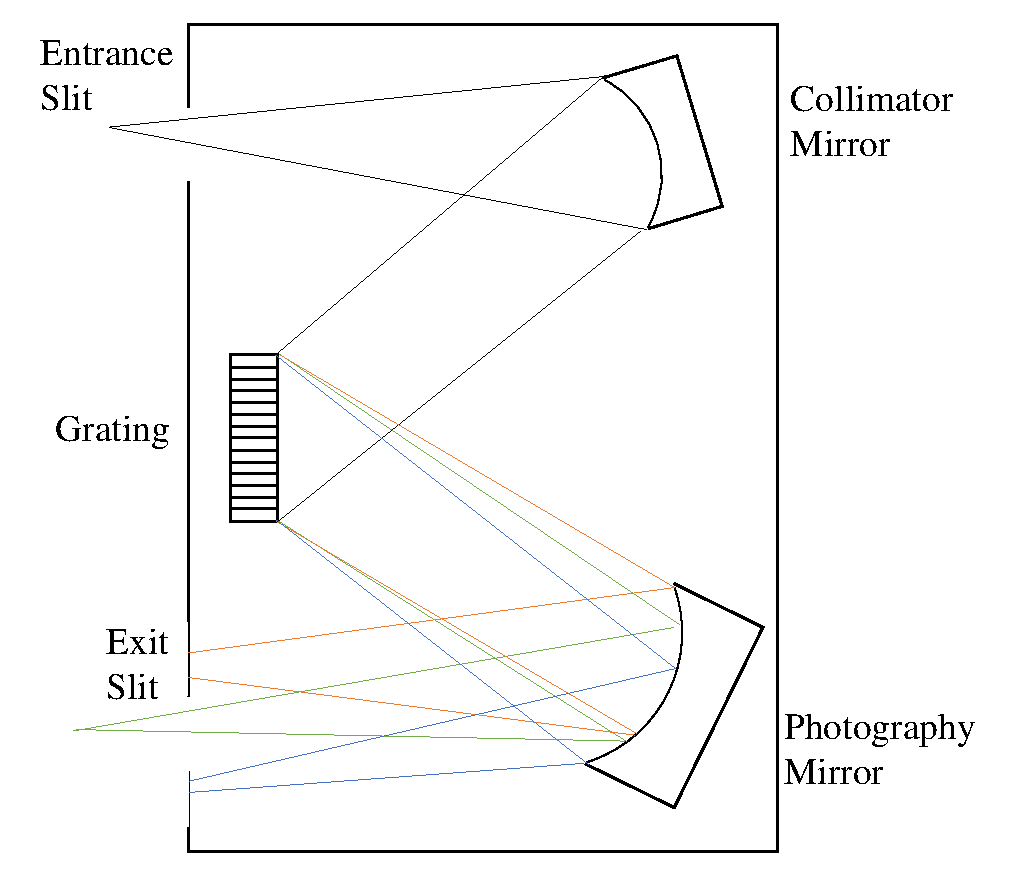
\includegraphics[clip,width=9cm]{monochromator.eps}
 \caption{シングルモノクロメーター概略図.}
 \label{fig_monochro1}
\end{figure}


\newpage
\subsubsection{回折格子}
回折格子は分散素子の一つである。今回の実験で用いた回折格子はブレーズド回折格子と呼ばれるものである。断面図を図\ref{fig_grating1}に示す\cite{Grating}。回折格子に平行光を入射すると、回折が起こる。単位長さ当たりの溝の数(グレーティング)が多いほど回折角が大きくなるため、得られるスペクトルの精度に差が出る。光の反射光とn次の回折光が重なるとき、つまり$\theta_{B}=\frac{\alpha-\beta}{2}$を満たすとき、その光は大きく検出される。その光の波長をブレーズ波長と呼ぶ。ブレーズ波長は回折格子ごとに特有の値であるため、実験の際はグレーティングとブレーズ波長の両方を考慮して回折格子を選ぶ必要がある。

\begin{figure}[h]
 \centering
 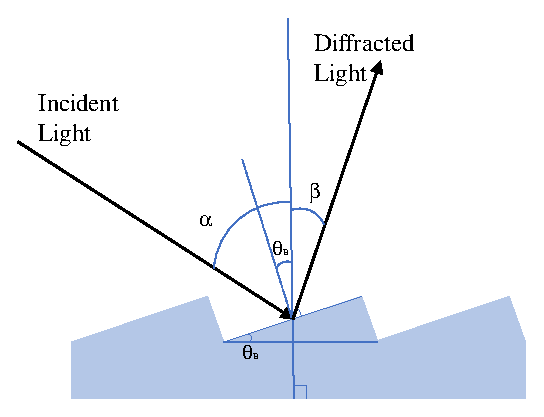
\includegraphics[clip,width=10cm]{grating.eps}
 \caption{ブレーズド回折格子断面図.}
 \label{fig_grating1}
\end{figure}

\subsubsection{CCD}
CCDの受光部分は平面上に光検出素子を並べたものである。光検出素子はpn接合の半導体で、光が当たるとp側にホール、n側に電子が移動し電荷をもつ。このようにして光を電荷に変換してデータへ変換している。この電荷を隣り合った素子へと伝えていく構造になっているため、電荷結合素子(Charge Coupled Device)の名前がついている\cite{CCD}。今回用いたCCDの光検出素子の大きさは、縦20 $\upmu$m、横20 $\upmu$mのものである。光検出素子が検出できる光の強さには限界がある。限界を超える強さの光を長時間照射すると光検出素子が破損する恐れがある。%1340個

\newpage
\subsubsection{光ファイバー}
光ファイバーは、光信号を伝送する伝送路として用いられる細い線である。光ファイバーの概略図を図\ref{fig_fibor1}に示す。光ファイバーは、屈折率の高いコアとそれを覆うクラッドからなっている。コア内で光が全反射を繰り返すことで、光を遠くへ伝送することが可能になっている\cite{Fibor}。今回の実験では、図\ref{fig_fibor1}のように光ファイバーはコアが10個縦に配列されたものを用いた。

\begin{figure}[h]
 \centering
 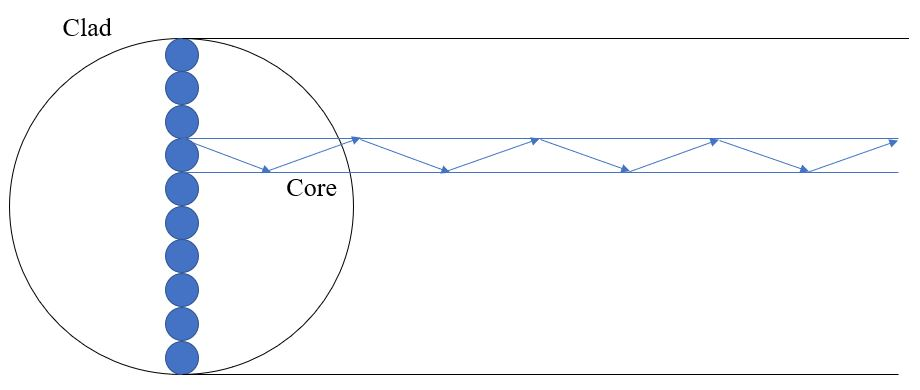
\includegraphics[clip,width=10cm]{start_fibor.jpg}
 \caption{ファイバー概略図.}
 \label{fig_fibor1}
\end{figure}

\subsubsection{半導体レーザー}
光子と半導体の電子との相互作用は、図\ref{fig_semi1}のように大きく以下の三つに分けられる。

\begin{figure}[ht]
 \centering
 \begin{tabular}{c}

  % 1
  \begin{minipage}{0.33\hsize}
   \centering
   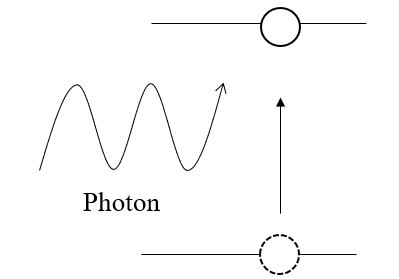
\includegraphics[clip, width=4.5cm,height=3cm]{start_photon_abs.jpg}
   \hspace{1.6cm} [1]吸収
  \end{minipage}

  % 3
  \begin{minipage}{0.33\hsize}
   \centering
   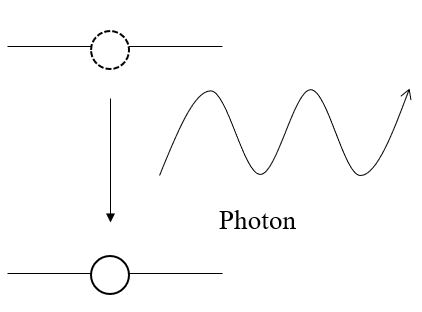
\includegraphics[clip, width=4.5cm]{start_photon_rel.jpg}
   \hspace{1.6cm} [2]放出
  \end{minipage}

  % 2
  \begin{minipage}{0.33\hsize}
   \centering
   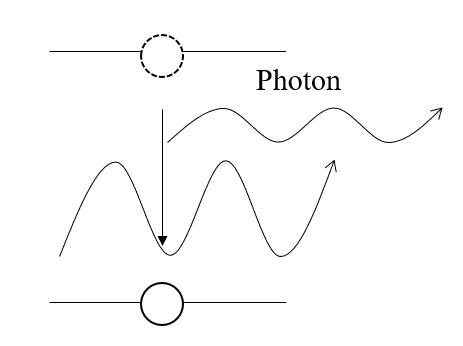
\includegraphics[clip, width=4.5cm]{start_photon_ind.jpg}
   \hspace{1.6cm} [3]誘導放出
  \end{minipage}
 \end{tabular}
 \caption{光子と半導体中の電子との相互作用.}
 \label{fig_semi1}

\end{figure}
%ここの表現をきっちりと
吸収は、エネルギーギャップよりも大きいエネルギーを持った一つの光子によって、価電子帯の電子が一つ励起される現象である。放出は、励起された電子が価電子帯へ戻るとき、そのエネルギーを光子として放出する現象である。誘導放出は、励起した電子と同じエネルギーを持つ光が入射したとき、その光によって励起した電子の放出が誘発される現象である。誘導放出で発生する光は、起因となった光と波長、位相、進行方向が同じであるため、起因となった光が強められる。これを利用したレーザーが半導体レーザーである。レーザー発振の概略図を図\ref{fig_laser1}に示す。
%ここ丁寧に(ヘクト3)

\begin{figure}[h]
 \centering
 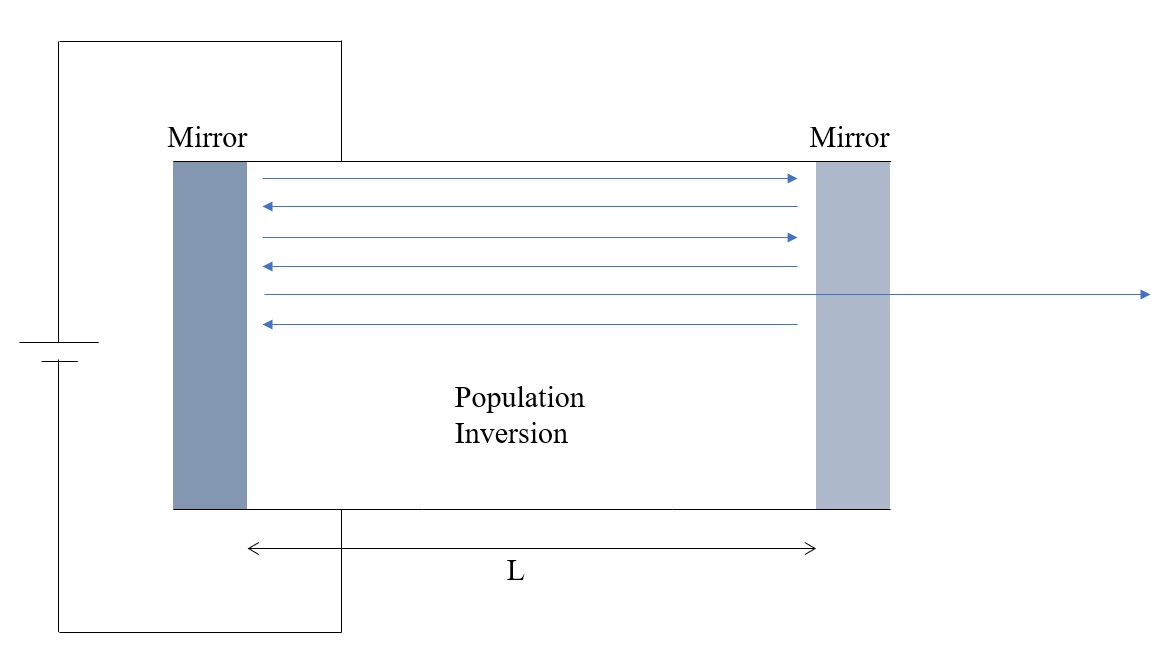
\includegraphics[clip,width=10cm]{start_semi_laser.jpg}
 \caption{レーザー発振概略図.}
 \label{fig_laser1}
\end{figure}

\newpage
半導体を、2枚の平行なミラーで挟む。片方のミラーは、照射された光をすべて反射し、もう片方は、照射された光の一部を透過させる。半導体に電圧を加え、半導体中の電子の半分以上を励起させる。この状態を反転分布状態と呼ぶ。ミラーに垂直な光が発生すると、その光はミラー間を往復し、誘導放出を繰り返し起き、起因となった光の強度が増える。光の波長が$n\lambda=2\mathrm{L}$ (n:自然数)を満たすとき、ミラー間を何度往復しても、ミラーの透過以外で光は減衰しない。強められた光の一部が、片方のミラーを透過することで、光源として使用できる。この光は、波長、位相、進行方向が常に一定なので、安定した光源として使用できる。

\newpage
%筒に入った反転分布状態の半導体を、透過率が100\%の鏡と、100\%でない鏡で挟む。筒の内部で、鏡によって閉じ込められた光が誘導放出を繰り返す。そうして得られる利得を片方のミラーから出すことで、安定した光の供給が可能になる。

\newpage
\subsubsection{ガスレーザー}
気体の原子の電子準位を利用したレーザーがある。一例としてHe-Neレーザーの発光原理を説明する。He-Neレーザーは、気体のヘリウムとネオンを用いて発光する。まず、気体中のヘリウム原子を励起させる。それが基底状態のネオン原子と衝突することで、ネオン原子が励起される。励起されたネオン原子が、基底状態へ遷移するときに放出するエネルギーが光になる。ヘリウムとネオンのエネルギー準位を図\ref{fig_laser2}に示す\cite{HeNe}。

\begin{figure}[h]
 \centering
 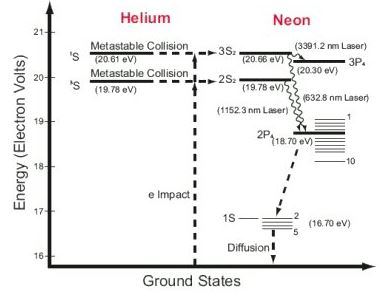
\includegraphics[clip,width=10cm]{start_gas_laser.jpg}
 \caption{ヘリウムとネオンのエネルギー準位.}
 \label{fig_laser2}
\end{figure}

He-Neレーザーに期待するのは波長632.8 nmの光だが、異なる波長の光も同時に放出される。そのため、He-Neレーザーを励起光源として用いるときは、干渉フィルターを用いてほかの波長の光を遮断する必要がある。
%He-Neレーザーのメーカーを確認してから、干渉フィルターもここで言及

\newpage
\subsection{正確なデータを得るための補正}
\subsubsection{波長校正}

分光器では入射スリットから入射した光のスペクトルを得ることができる。そのスペクトルを用いて議論を行うためには、分光器から正しいデータが得られることを確認しておく必要がある。そのために行う作業が波長校正である。水銀灯のような、発光波長が既に知られている光源を用意する。分光器を用いてその光の波長を得て、既知の波長と照らし合わせる。ズレが生じていた場合はそれを校正する。

\subsubsection{分光器感度補正}
分光器では入射スリットから入射した光のスペクトルを得ることができる。しかし、入射光の波長によって分光器の感度が異なるため、得られたスペクトルは入射光のスペクトルそのものではない。分光計の感度曲線の一例を図\ref{fig_sensitivity1}に示す。

\begin{figure}[h]
 \centering
 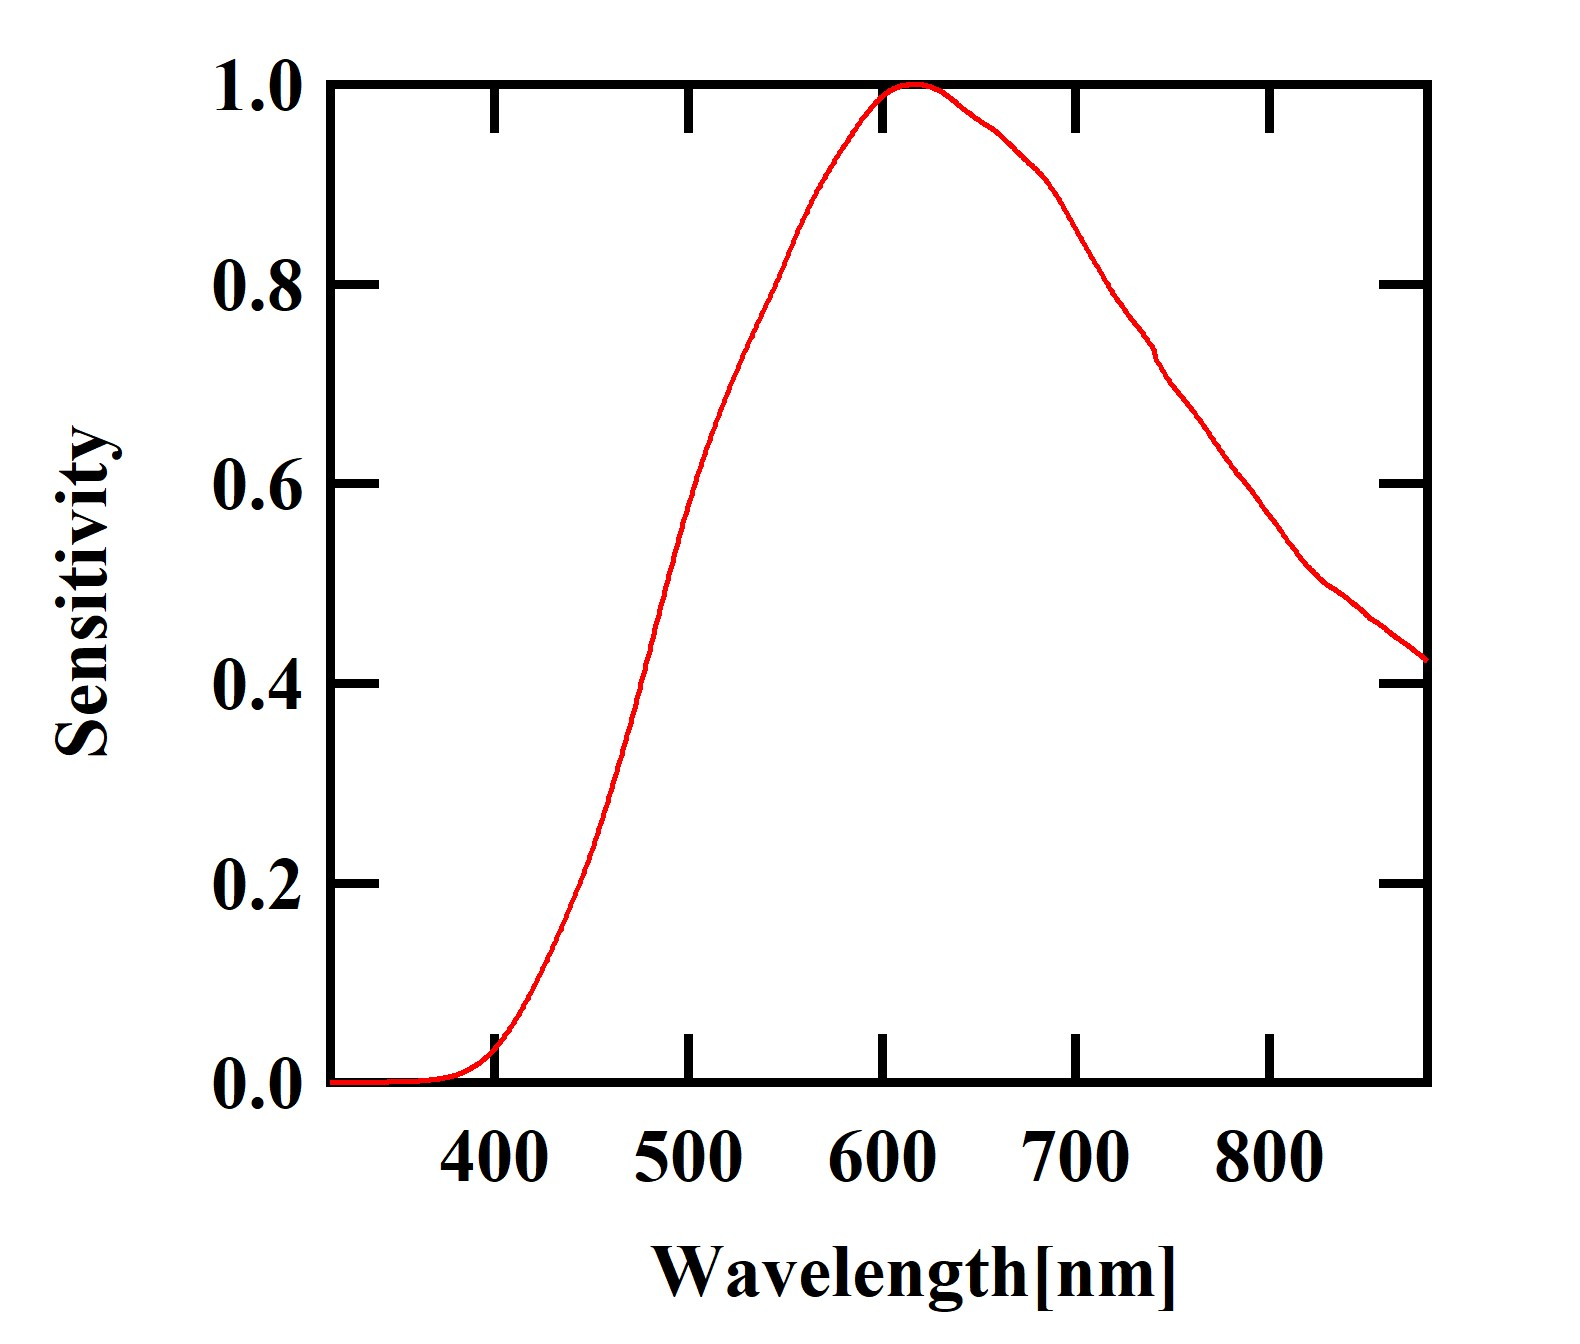
\includegraphics[clip,width=10cm]{start_sensitivity.jpg}
 \caption{分光器 SP2300 150 g/mmの感度曲線.}
 \label{fig_sensitivity1}
\end{figure}

グラフを見ると、波長が600 nmの光はデータにほぼ100 \%反映できているが、40 nmでは10 \%も反映できていないことがわかる。分光器の感度による影響をなくすため、得られたスペクトルを補正する必要がある。あらかじめ分光器感度補正曲線がわかっていれば、分光器感度補正が可能である。

\subsubsection{フィルター感度補正}

分光器を用いて光のスペクトルを得たいとき、他の光はできるだけ入射させたくない。そのため、光学系において、ファイバーの開口部にフィルターを設置して、他の光を遮断する。しかし、フィルターによっては、透過率に波長依存性があるため、本来遮断しない波長域の光が減衰してしまうことがある。分光器の感度補正と同様に、あらかじめフィルターの特性がわかっていれば、補正をかけることでフィルターの影響をなくすことができる。

\newpage
\subsection{半導体の発光の特性}

\subsubsection{バンド間発光}
半導体は価電子帯と伝導帯の間にエネルギーギャップを持つ。半導体のバンド図を図\ref{fig_band1}に示す。エネルギーギャップよりも大きなエネルギーを持った光子が半導体に照射されると、そのエネルギーによって価電子帯の電子が伝導帯に励起される。励起された電子は時間が経過すると価電子帯の正孔と再結合するが、その時にエネルギーギャップ分のエネルギーを放出する。このエネルギーが光子として放出される現象が、バンド間の発光である。電子を励起する光子の数と、放出された光子は同じ数であるため、発光強度は励起光の強度に比例する。発光の強度を、波長またはエネルギーを横軸としてグラフにしたものがバンド間発光のスペクトルである。%%例として、室温におけるGaAsの発光スペクトルを図\ref{fig_lumine1}に示す。

\begin{figure}[h]
 \centering
 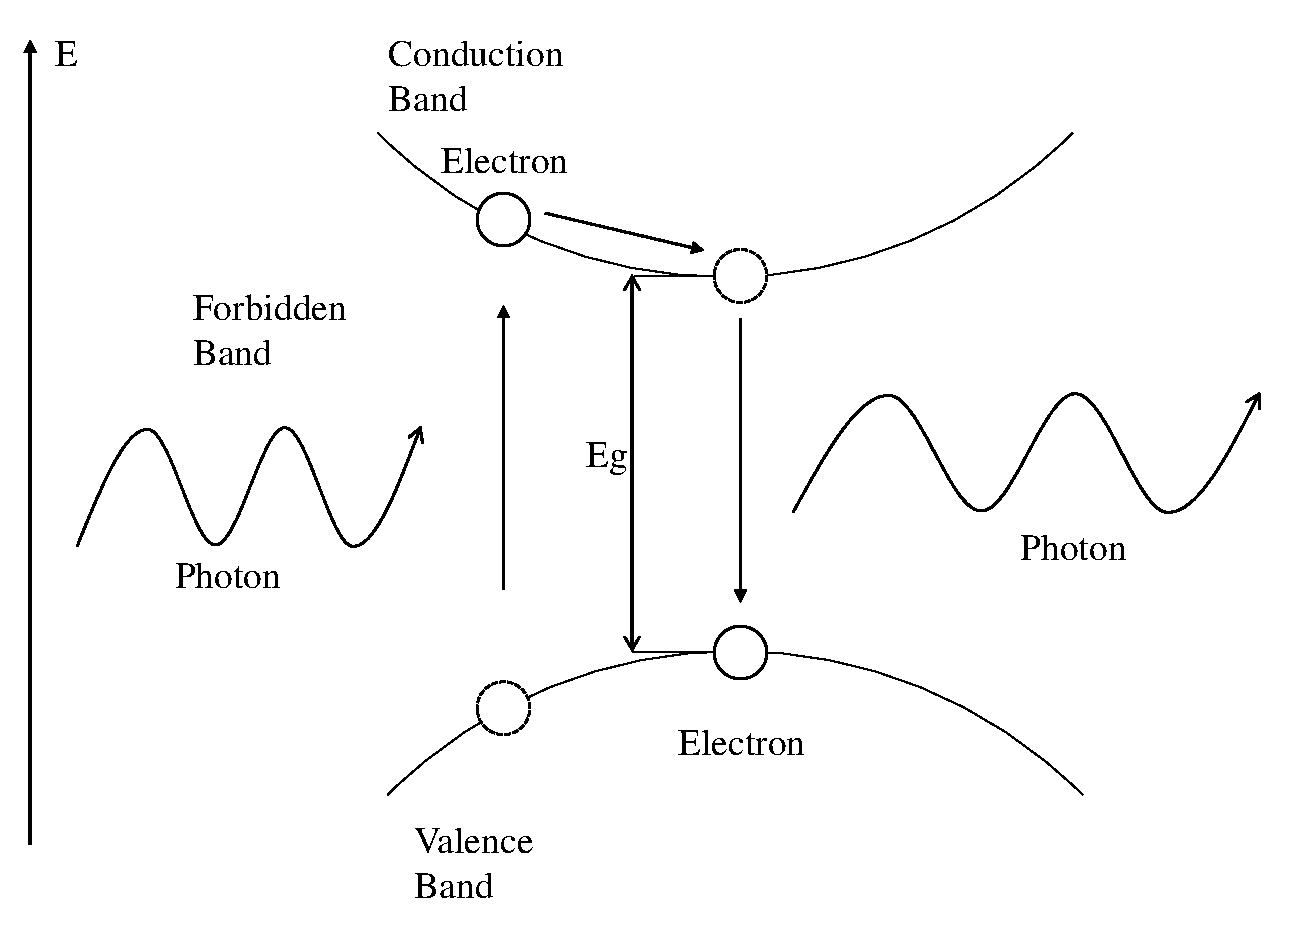
\includegraphics[clip,width=10cm]{start_semiconductor.eps}
 \caption{半導体のバンド図.}
 \label{fig_band1}
\end{figure}

温度が下がると、半導体のエネルギーギャップが大きくなる。エネルギーギャップの温度依存性は

\begin{equation}
 E(T)=E(0)-\frac{\upalpha T^{2}}{T+\upbeta}
 \label{eq_varshni}
\end{equation}
で表される\cite{varshni}。これはVarshniの経験則と呼ばれる。$\upalpha$と$\upbeta$は試料ごとに定まる定数である。

%\subsubsection{エネルギーギャップの温度依存性}


\newpage
\subsubsection{量子井戸}
バルク試料においては、電子は3次元方向に自由に動くことができる。しかし、1方向の幅を、電子の波長よりも小さくなるまで縮めると、電子は2次元的方向にしか移動できなくなる。それを、バンドギャップが大きい物質で挟むと、電子のエネルギーは量子化されて離散的な準位しか取れなくなる。このように1次元方向に閉じ込めが行われた物質を量子井戸と呼ぶ。量子井戸のバンド図を図\ref{fig_qw1}に示す。

\begin{figure}[h]
 \centering
 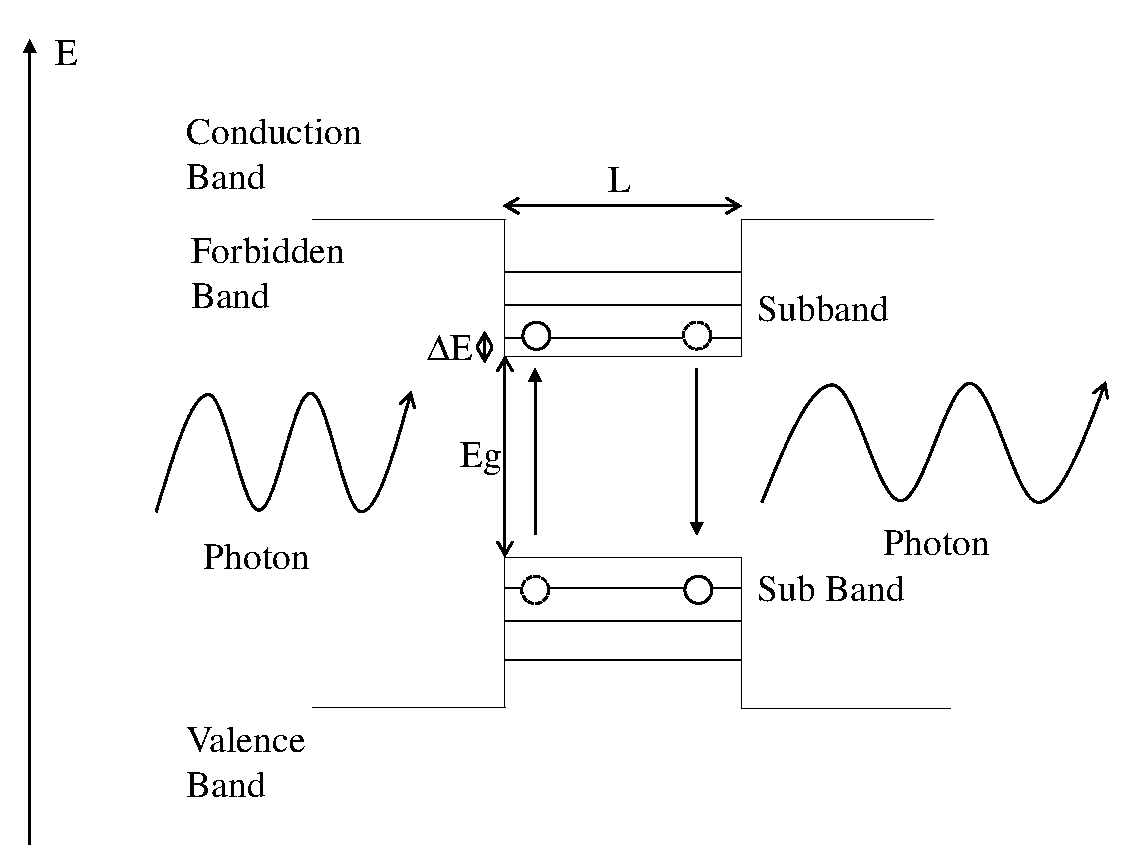
\includegraphics[clip,width=10cm]{start_subband.eps}
 \caption{量子井戸のバンド図.}
 \label{fig_qw1}
\end{figure}

量子井戸に形成された、離散的なエネルギー準位をサブバンドと呼ぶ。サブバンドが形成された量子井戸では、価電子帯と伝導帯の電子の移動は、価電子帯のサブバンドのうちの最もエネルギー準位が高いものと、伝導帯のサブバンドのうちの最もエネルギー準位の低いものとの間で行われる。また、それらのサブバンドのエネルギー準位と、物質の元々のエネルギー準位との差$\Delta E$は、井戸幅$L$を用いて、
\begin{equation}
 \Delta E=\frac{\mathrm{\hbar}^{2}\uppi^{2}}{2mL^{2}}
 \label{eq_qw}
\end{equation}
で表される。1次元的閉じ込めがなされたのが量子井戸だが、2次元的なものは量子細線、3次元的なものは量子ドットと呼ばれる。

\newpage
\subsubsection{励起子}
励起子は、伝導帯に励起された電子と、価電子帯に空いた正孔がクーロン引力によって束縛された状態である。励起子の概略図を図\ref{fig_exciton1}に、エネルギー準位を図\ref{fig_exciton2}に示す。図\ref{fig_exciton1}のような、電子-正孔対が結晶空間の中である程度の広がりを持っている励起子をワニエ型励起子と呼ぶ。また、この広がりを有効ボーア半径と呼ぶ。

\begin{figure}[h]
 \centering
 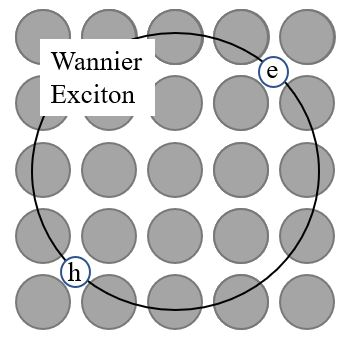
\includegraphics[clip,width=5cm]{start_exciton.jpg}
 \caption{ワニエ型励起子.}
 \label{fig_exciton1}
\end{figure}

\begin{figure}[h]
 \centering
 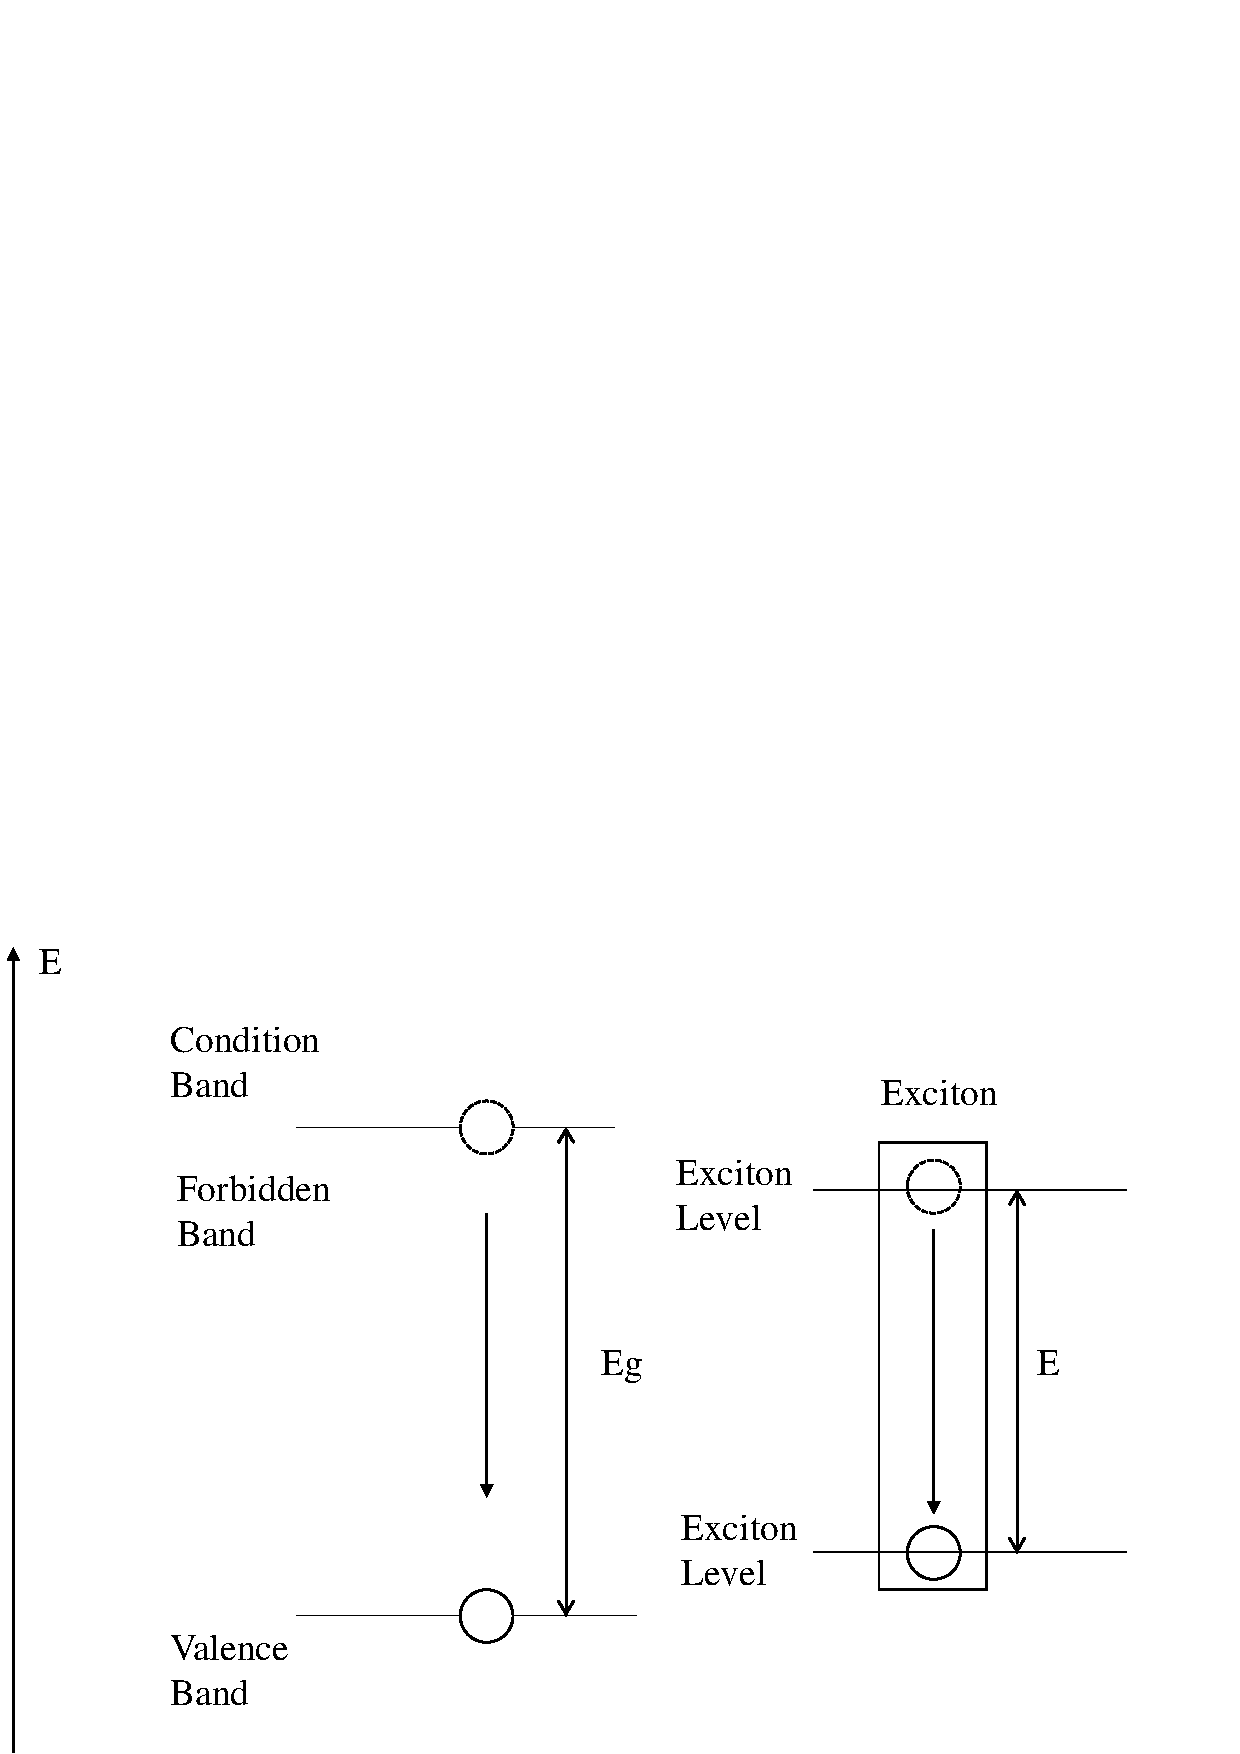
\includegraphics[clip,width=10cm]{start_exciton_binding.jpg}
 \caption{励起子準位の概略図.}
 \label{fig_exciton2}
\end{figure}

励起子はクーロン束縛されているため、図\ref{fig_exciton2}のように、元々のバンドギャップエネルギーよりも束縛エネルギーの分だけエネルギー準位が低い状態にある。そのため、励起子が生成される物質の発光スペクトルでは、励起子の影響が表れる。

\newpage
\section{分光計の扱い方及び半導体の発光スペクトルの観測方法}

\subsection{実験1.分光器のスリット幅とスペクトル分解能の関係}


測定で用いた光学系を図\ref{fig_system1}に示す。

\begin{figure}[h]
 \centering
 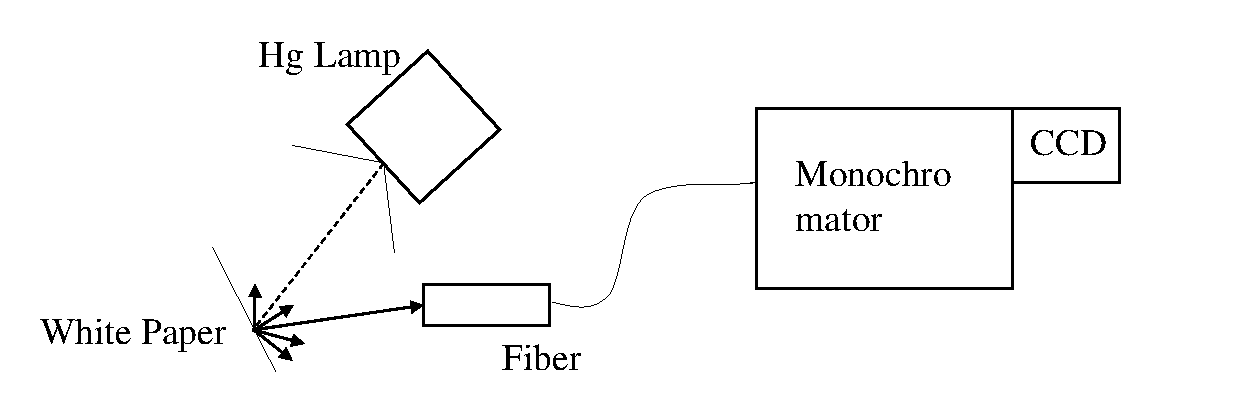
\includegraphics[clip,width=10cm]{start_system1.eps}
 \caption{実験1の光学系.}
 \label{fig_system1}
\end{figure}

水銀灯から等方的に放射された光を白紙に一度当てて、散乱した光をファイバーを通して分光器まで送った。一度白紙にあてたのは、水銀灯の光が直接ファイバーに入り、光検出素子が破損することを防ぐためである。実験条件を表\ref{col_1}に示す。分光器の回折格子は、300 g/mmのものと1200 g/mmの2種類を用いた。スリット幅を変えてゆき、発光スペクトルを測定した。

\begin{table}[ht]
 \centering
 \caption{実験1の実験条件.}
 \begin{tabular}{lc}\hline
  \multicolumn{2}{c}{実験条件}      \\ \hline
  分光器の焦点距離 & 300 mm         \\
  中心波長         & 435 nm         \\
  露光時間         & 0.1 秒         \\
  積算回数         & 1 回           \\
  試料温度         & 19 ${}^\circ$C \\ \hline
 \end{tabular}
 \label{col_1}
\end{table}

%\begin{enumerate}
%	\item 図\ref{fig_system1}のように光学系を組んだ。
%	\item 分光器とPCを接続した。
%	\item 分光器の入射スリットの幅を30 $\upmu$mにした。使用する回折格子を300 g/mmに設定して分光器の波長校正を行った。
%	\item 中心波長を435 nmに設定した。
%	\item スリット幅を500 $\upmu$mまで開いた。そこから目盛で数えて-50 $\upmu$mまでスリット幅を狭めてゆき、それぞれのスリット幅で得られた水銀灯のスペクトルを記録した。露光時間は0.1 秒、積算回数は1 回とした。実験は室温で行った。
%	\item 2.から4.の手順を、使用する回折格子を1200 g/mmにして再度行った。
%\end{enumerate}

\newpage
\subsection{実験2.半導体試料の発光スペクトルの励起光強度依存性}
\subsubsection{実験2.1. CdSの発光スペクトルの励起光強度依存性}

%この実験で用いた試料は、厚さ0.5 mmのCdSの結晶である。
測定で用いた光学系を図\ref{fig_system2}に示す。

\begin{figure}[h]
 \centering
 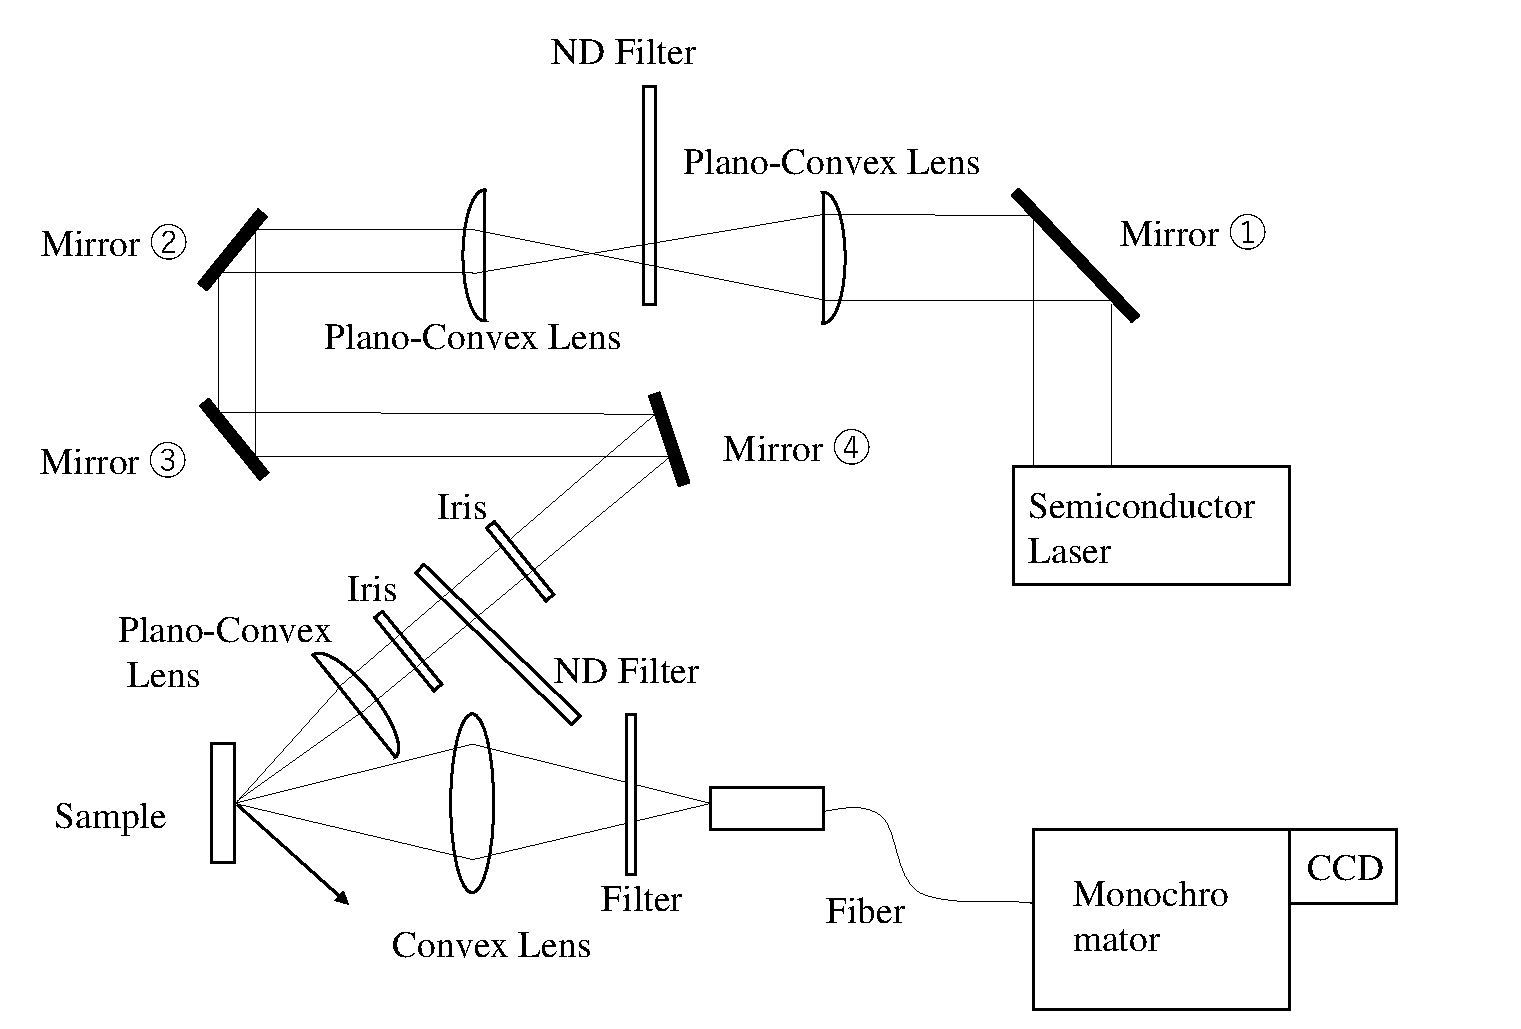
\includegraphics[clip,width=10cm]{start_system2.eps}
 \caption{実験2.1の光学系.}
 \label{fig_system2}
\end{figure}

波長450 nmのレーザーを試料に照射し、試料の発光を凸レンズを用いてファイバーの開口部に集め、ファイバーを通して分光器まで伝送した。ファイバーの開口部に、レーザーの散乱光などが入らないようフィルターS76-Y48を設置した。レーザー出射後の励起光を、2枚の片凸レンズを用いて平行光にした。試料に当たる光を抑えるため、NDフィルターを用いて光量を減らした。アイリス2つとミラー\centercircle{1}、\centercircle{2}を用いて光路を調整し、片凸レンズを用いて試料に一点で光が当たるよう光を絞った。実験条件を表\ref{col_2.1}に示す。励起光強度を変えてゆき、発光スペクトルを測定した。

\begin{table}[ht]
 \centering
 \caption{実験2.1の実験条件.}
 \begin{tabular}{lc}\hline
  \multicolumn{2}{c}{実験条件}         \\ \hline
  分光器の焦点距離 & 300 mm            \\
  回折格子         & 150 g/mm          \\
  中心波長         & 600 nm            \\
  スリット幅       & 30 $\upmu$m       \\
  露光時間         & 0.01 秒           \\
  積算回数         & 5 回              \\
  実験試料         & CdS結晶(d=0.5 mm) \\
  試料温度         & 20 ${}^\circ$C    \\ \hline
 \end{tabular}
 \label{col_2.1}
\end{table}

%\begin{enumerate}%
%	\item 図\ref{fig_system2}のように光学系を組んだ。
%	\item 分光器とPCを接続した。
%	\item 使用する回折格子を300 g/mmに設定して分光器の波長校正を行った。
%	\item 分光器の入射スリットの幅を30 $\upmu$mにし、中心波長を600 nmに設定した。
%	\item レーザーを起動し、試料にあたる励起光の強度が7 mWになるようNDフィルターを調節した。そこから1 mWまで励起光強度を減らしてゆき、それぞれの強度で得られた試料の発光スペクトルを記録した。露光時間は0.01 秒、積算回数は5 回とした。実験は室温で行った。
%\end{enumerate}

\newpage
\subsubsection{実験2.2. GaAsの発光スペクトルの励起光強度依存性}

%この実験で用いた試料は、厚さ0.5 mmのGaAsの結晶である。
測定で用いた光学系を図\ref{fig_system3}に示す。

\begin{figure}[h]
 \centering
 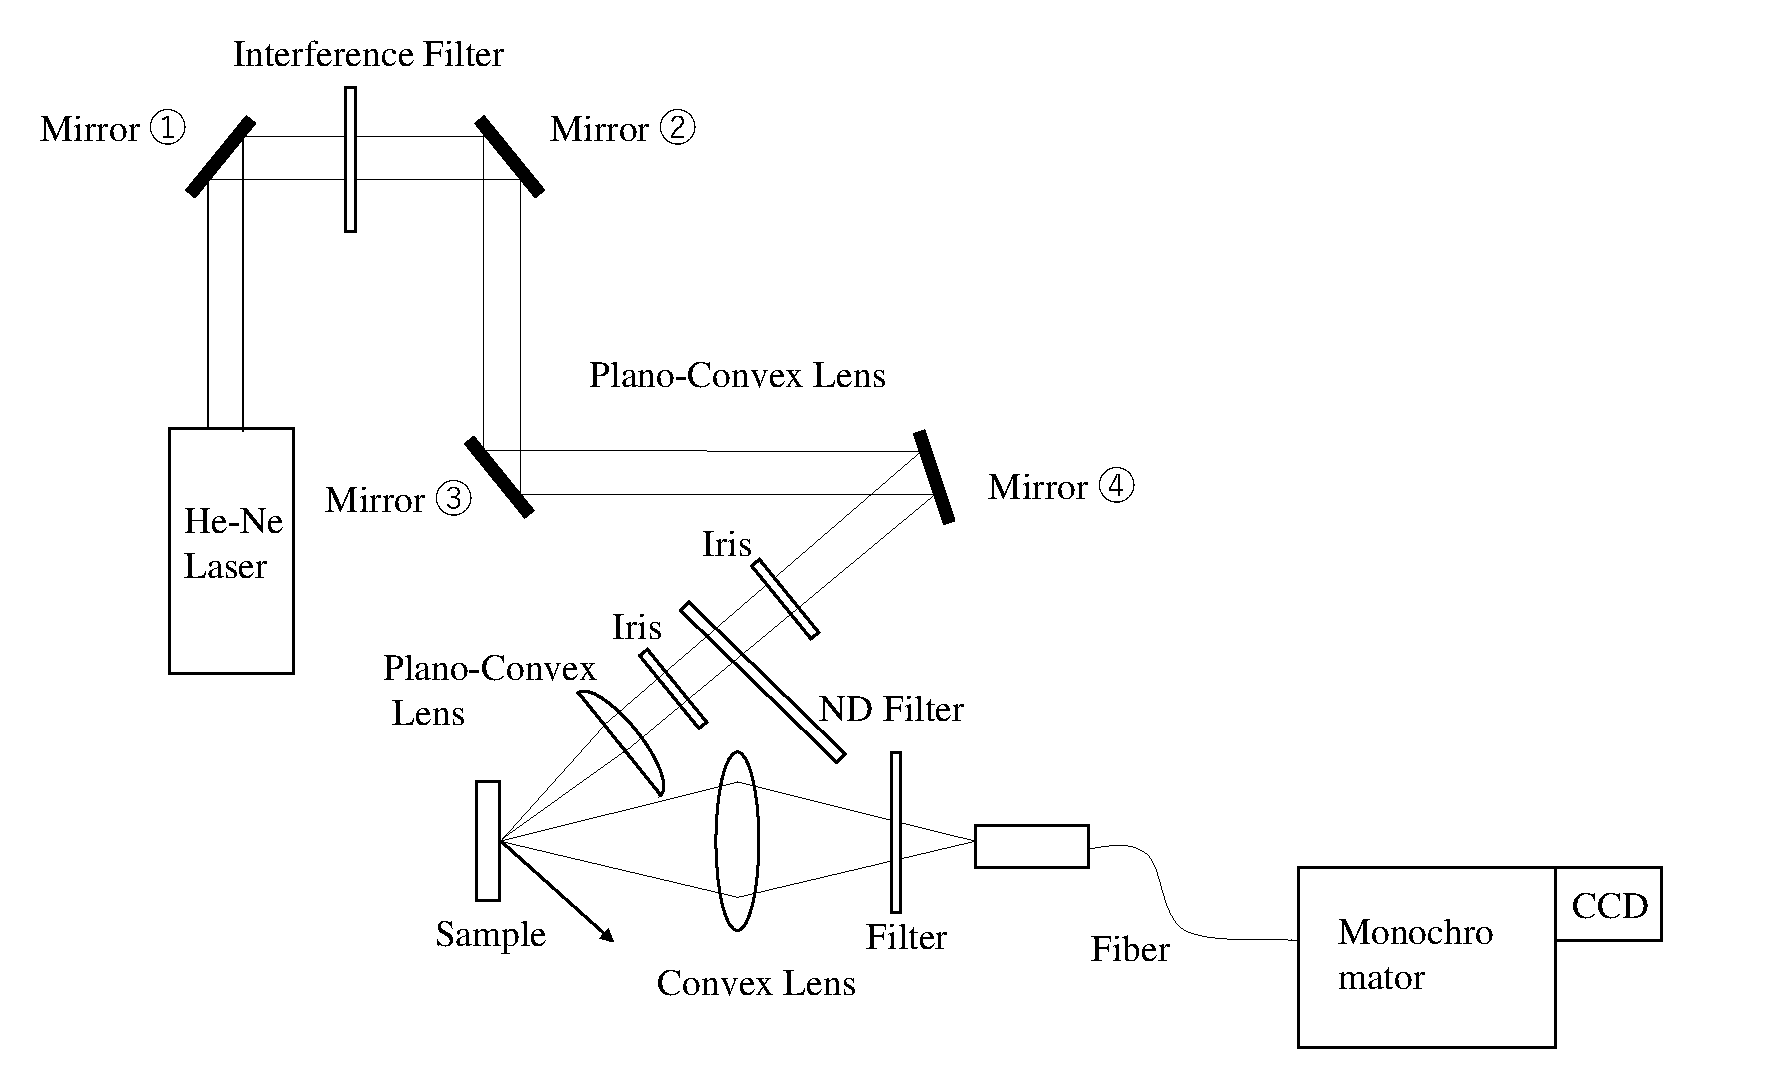
\includegraphics[clip,width=10cm]{start_system3.eps}
 \caption{実験2.2の光学系.}
 \label{fig_system3}
\end{figure}

%波長632.8 nmのHe-Neレーザーを試料に照射し、試料の発光を凸レンズを用いてファイバーの開口部に集め、ファイバーを通して分光器まで送った。ファイバーの開口部に、レーザーの散乱光などが入らないようフィルターFGL780Sを設置した。He-Neレーザーからの光のうち、波長632.8 nmの光以外の光をカットするため、干渉フィルターを用いた。アイリス2つと試料から遠い2枚のミラーを用いて光路を調整し、片凸レンズを用いて試料に一点で光が当たるよう光を絞った。試料によるレーザーの反射光がファイバーに入らないよう試料の向きを調整した。
ミラー\centercircle{3}から分光器までの光学系は図\ref{fig_system2}と同様である。励起光源にHe-Neレーザーを用いた。波長632.8 nmの光以外をカットするため、干渉フィルターを用いた。実験条件を表\ref{col_2.2}に示す。励起光強度を変えてゆき、発光スペクトルを測定した。

\begin{table}[ht]
 \centering
 \caption{実験2.2の実験条件.}
 \begin{tabular}{lc}\hline
  \multicolumn{2}{c}{実験条件}          \\ \hline
  分光器の焦点距離 & 300 mm             \\
  回折格子         & 300 g/mm           \\
  中心波長         & 850 nm             \\
  スリット幅       & 30 $\upmu$m        \\
  露光時間         & 10 秒              \\
  積算回数         & 5 回               \\
  実験試料         & GaAs結晶(d=0.5 mm) \\
  試料温度         & 20 ${}^\circ$C     \\ \hline
 \end{tabular}
 \label{col_2.2}
\end{table}

%\begin{enumerate}
%	\item 図\ref{fig_system3}のように光学系を組んだ。
%	\item 分光器とPCを接続した。
%	\item 使用する回折格子を300 g/mmに設定して分光器の波長校正を行った。
%	\item 分光器の入射スリットの幅を30 $\upmu$mにし、中心波長を850 nmに設定した。
%	\item レーザーを起動し、試料にあたる励起光の強度が5 mWになるようNDフィルターを調節した。そこから1 mWまで励起光強度を減らしてゆき、それぞれの強度で得られた試料の発光スペクトルを記録した。露光時間は10 秒、積算回数は5 回とした。実験は室温で行った。
%\end{enumerate}

\newpage
\subsubsection{実験2.3. GaAs/AlGaAs量子井戸の発光スペクトルの励起光強度依存性}

測定で用いた光学系を図\ref{fig_system4}に示す。

\begin{figure}[h]
 \centering
 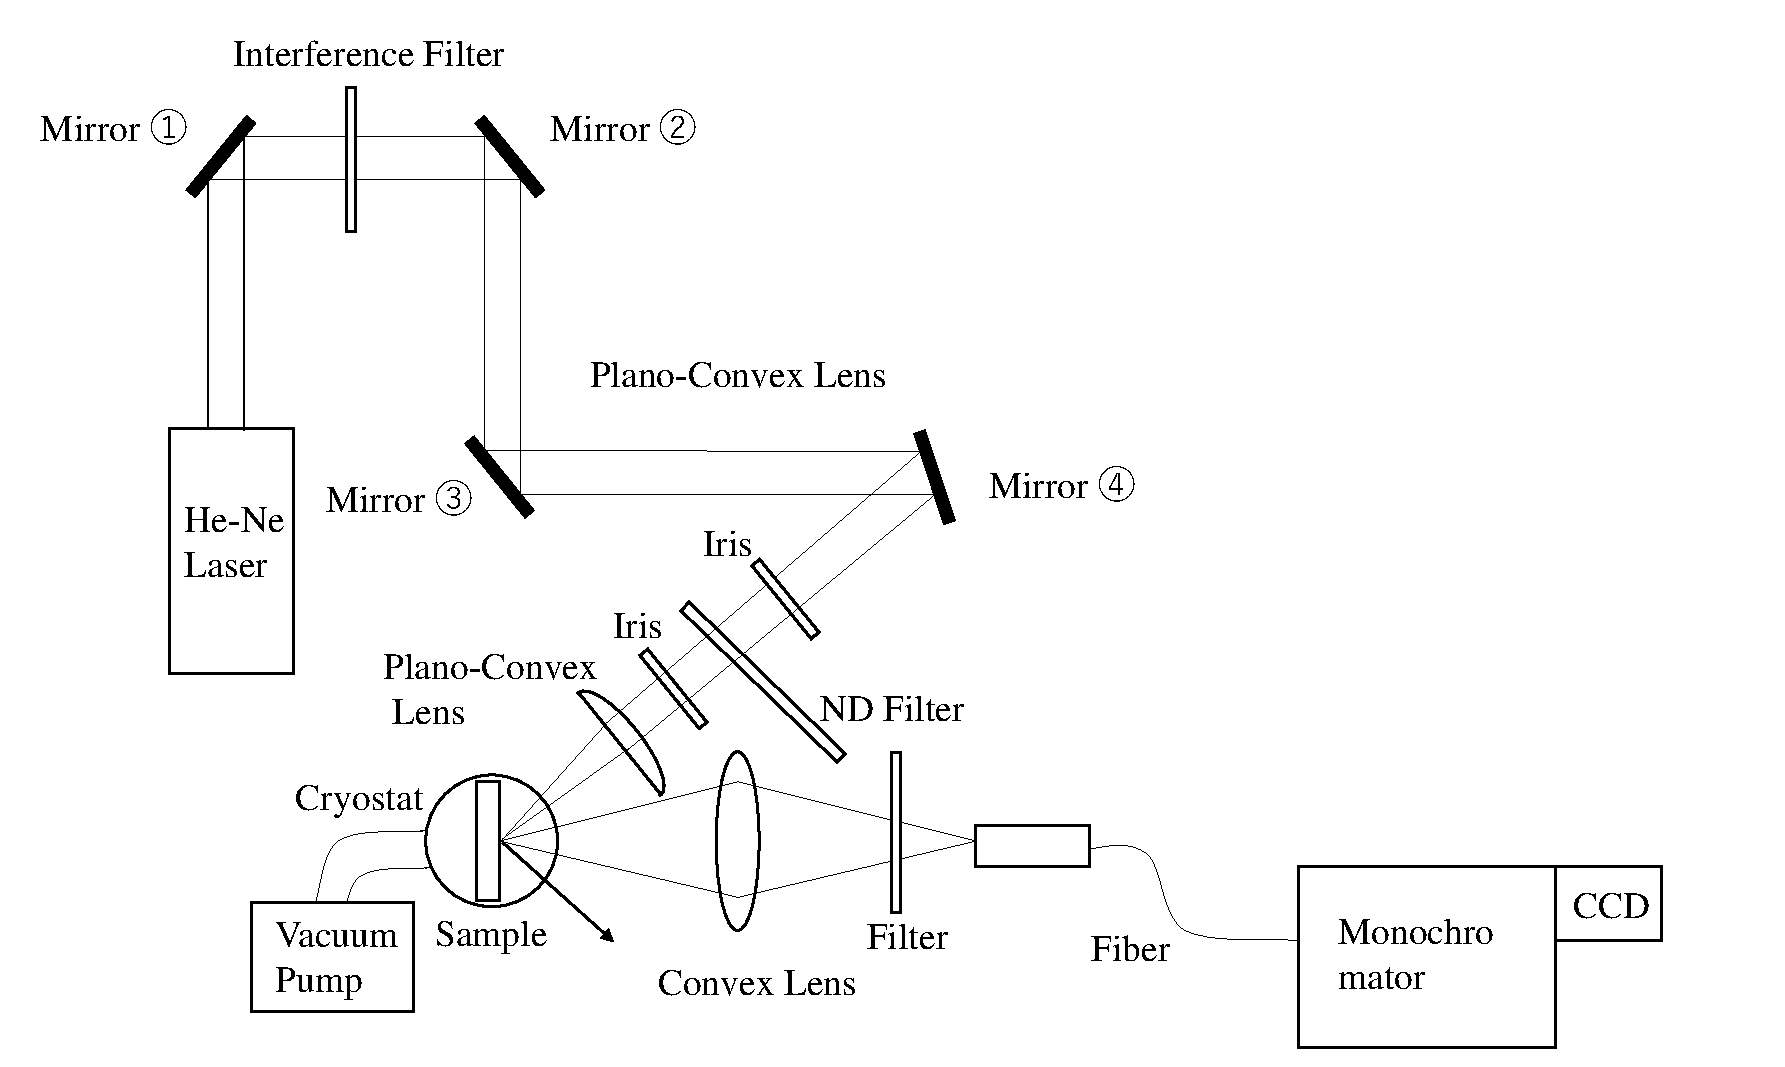
\includegraphics[clip,width=10cm]{start_system4.eps}
 \caption{実験2.3の光学系.}
 \label{fig_system4}
\end{figure}

試料部分以外の光学系は図\ref{fig_system3}と同様である。77 Kの低温にするため、クライオスタットを用いた。銀ペーストを用いて試料をクライオスタットに固定した。試料室内を真空にひくため、真空ポンプとクライオスタットを接続した。表\ref{col_2.3}の実験条件の下、試料の温度ごとに、励起光強度を変えてゆき、発光スペクトルを測定した。試料の温度は、室温と77 Kの2通りである。

\begin{table}[ht]
 \centering
 \caption{実験2.2の実験条件.}
 \begin{tabular}{lc}\hline
  \multicolumn{2}{c}{実験条件}                                      \\ \hline
  分光器の焦点距離 & 300 mm                                         \\
  回折格子         & 300 g/mm                                       \\
  中心波長         & 850 nm                                         \\
  スリット幅       & 30 $\upmu$m                                    \\
  露光時間         & 0.1 秒                                         \\
  積算回数         & 5 回                                           \\
  実験試料         & $\mathrm{GaAs/Al_{0.3}Ga_{0.7}As}$多重量子井戸 \\ \hline
 \end{tabular}
 \label{col_2.3}
\end{table}

\newpage
試料の構造を図\ref{fig_algaas1}に示す。今回の試料は試料の$\mathrm{GaAs/Al_{0.3}Ga_{0.7}As}$多重量子井戸である。GaAs基板の上に、井戸幅が5,6,7,8,9,10 nmの$\mathrm{GaAs/Al_{0.3}Ga_{0.7}As}$量子井戸が積層されている。それぞれの量子井戸の構造について、井戸幅10 nmの量子井戸を例に説明する。幅10 nmのGaAsの薄膜5枚を、十分大きな厚さを持った$\mathrm{Al_{0.3}Ga_{0.7}As}$結晶で挟む。他の井戸幅の量子井戸についても同様である。

\begin{figure}[h]
 \centering
 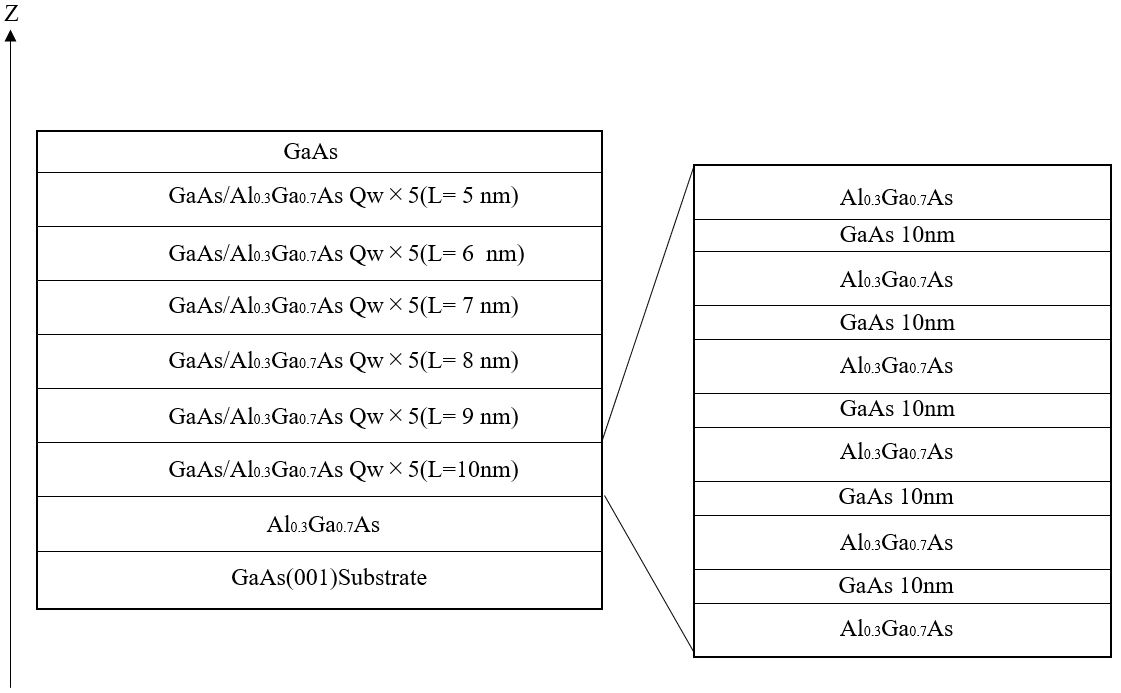
\includegraphics[clip,width=10cm]{start_AlGaAs.jpg}
 \caption{$\mathrm{GaAs/Al_{0.3}Ga_{0.7}As}$多重量子井戸の構造.}
 \label{fig_algaas1}
\end{figure}

\newpage
%波長632.8 nmのHe-Neレーザーを試料に照射し、試料の発光を凸レンズを用いてファイバーの開口部に集め、ファイバーを通して分光器まで送った。ファイバーの開口部に、レーザーの散乱光などが入らないようフィルターFGL715Sを設置した。試料に当たる光を抑えるため、干渉フィルターを用いて光量を減らした。アイリス2つと試料から遠い2枚のミラーを用いて光路を調整し、片凸レンズを用いて試料に一点で光が当たるよう光を絞った。試料によるレーザーの反射光がファイバーに入らないよう試料の向きを調整した。

%\begin{enumerate}
%	\item 図\ref{fig_system4}のように光学系を組んだ。
%	\item 分光器とPCを接続した。
%	\item 使用する回折格子を300 g/mmに設定して分光器の波長校正を行った。
%	\item 分光器の入射スリットの幅を30 $\upmu$mにし、中心波長を850 nmに設定した。
%	\item 真空ポンプを用いてクライオスタットに$5.9\times10^{-4}$ Paの真空を引いた。
%	\item レーザーを起動し、試料にあたる励起光の強度が5 mWになるようNDフィルターを調節した。そこから1 mWまで励起光強度を減らしてゆき、それぞれの強度で得られた試料の発光スペクトルを記録した。露光時間は0.1 秒、積算回数は5  回とした。実験は室温で行った。
%	\item クライオスタットに液体窒素を注ぎ、6.の手順を、実験条件を変えて再度行った。励起光の強度が250 $\upmu$WになるようNDフィルターを調節した。そこから10 $\upmu$Wまで励起光強度を減らしてゆき、それぞれの強度で得られた試料の発光スペクトルを記録した。露光時間は0.01 秒、積算回数は1回とした。試料を冷やした後の温度は77 K、クライオスタット中は$2.1\times10^{-4}$ Paの真空になっていた。
%\end{enumerate}

\newpage
\section{分光器の分解能及び半導体の発光スペクトルの解析}
\subsection{実験1. 分光器のスリット幅とスペクトル分解能の関係}

\begin{enumerate}%箇条書き環境下では文頭では自力で空白を入れる
 \item 300 g/mmの回折格子を用いた測定

       300 g/mmの回折格子を用いた時の、分光器のスリット幅とスペクトル幅の関係を図\ref{fig_300spectrum1}に示す。

       \begin{figure}[ht]
        \centering
        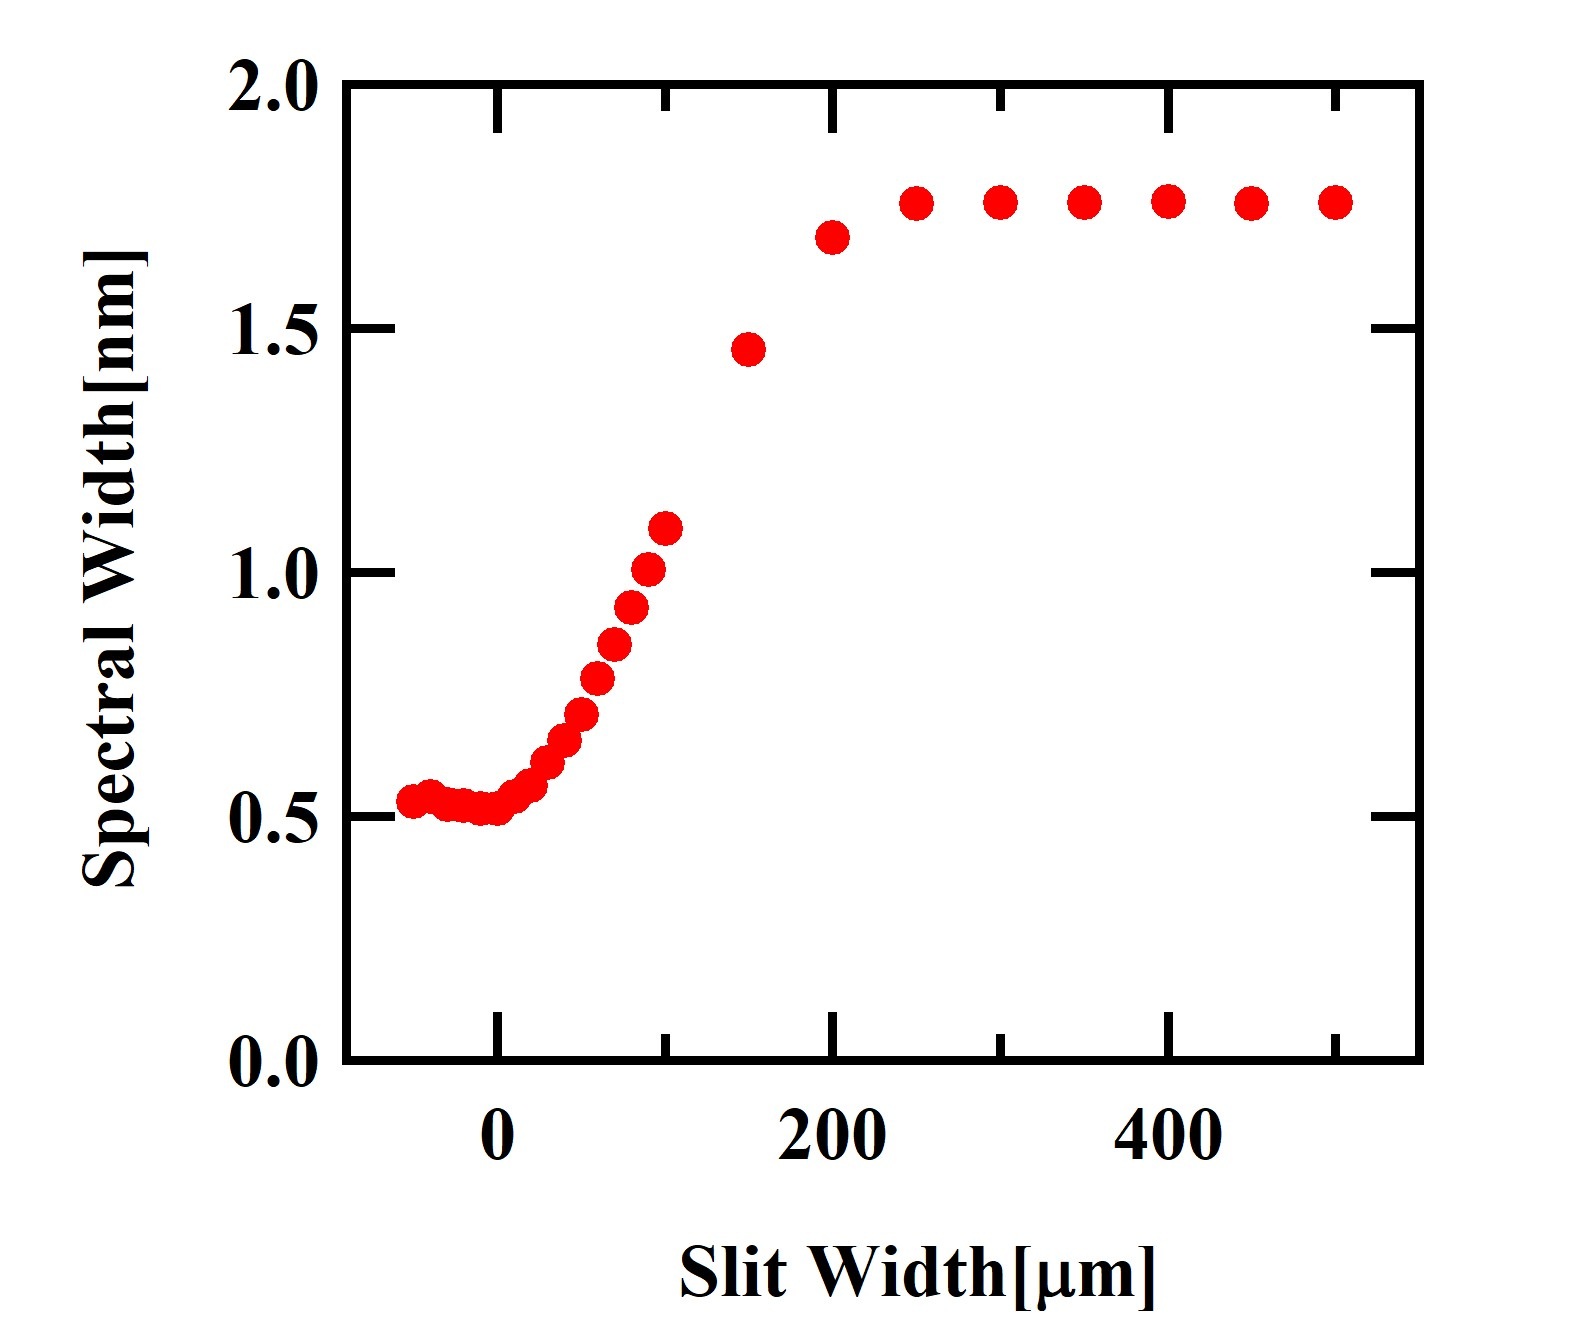
\includegraphics[clip,width=9cm]{start1_300Spectrum.jpg}
        \caption{300 g/mmの回折格子における分光器のスリット幅とスペクトル幅の関係.}
        \label{fig_300spectrum1}
       \end{figure}


       縦軸は水銀灯の発光スペクトルのスペクトル幅、横軸はスリット幅である。スリット幅が大きくなると、スペクトル幅が広がっているのがわかる。
       %入射スリットの目盛に負の値が存在するのは、入射スリットを操作するつまみに遊びがあるためである。スリット幅が0 $\upmu$mになったスリットはそれ以上閉じない。しかし、スリットを過剰に閉めると破損するため、つまみが空回りするのが、負の値の目盛である。ここでは、得られたスペクトルの半値全幅をスペクトル幅とした。
       %ここ言い回し決まったら黒字化。
       \\
       分解能$R$は$R=\lambda/\Updelta\lambda$で表される。観測した波長は435.835 nmである。ここでは$\lambda$は定まっているので、分解能とスペクトル幅は反比例の関係にある。スリット幅と分解能の関係を図\ref{fig_300resolution1}に示す。
       \newpage

       \begin{figure}[ht]
        \centering
        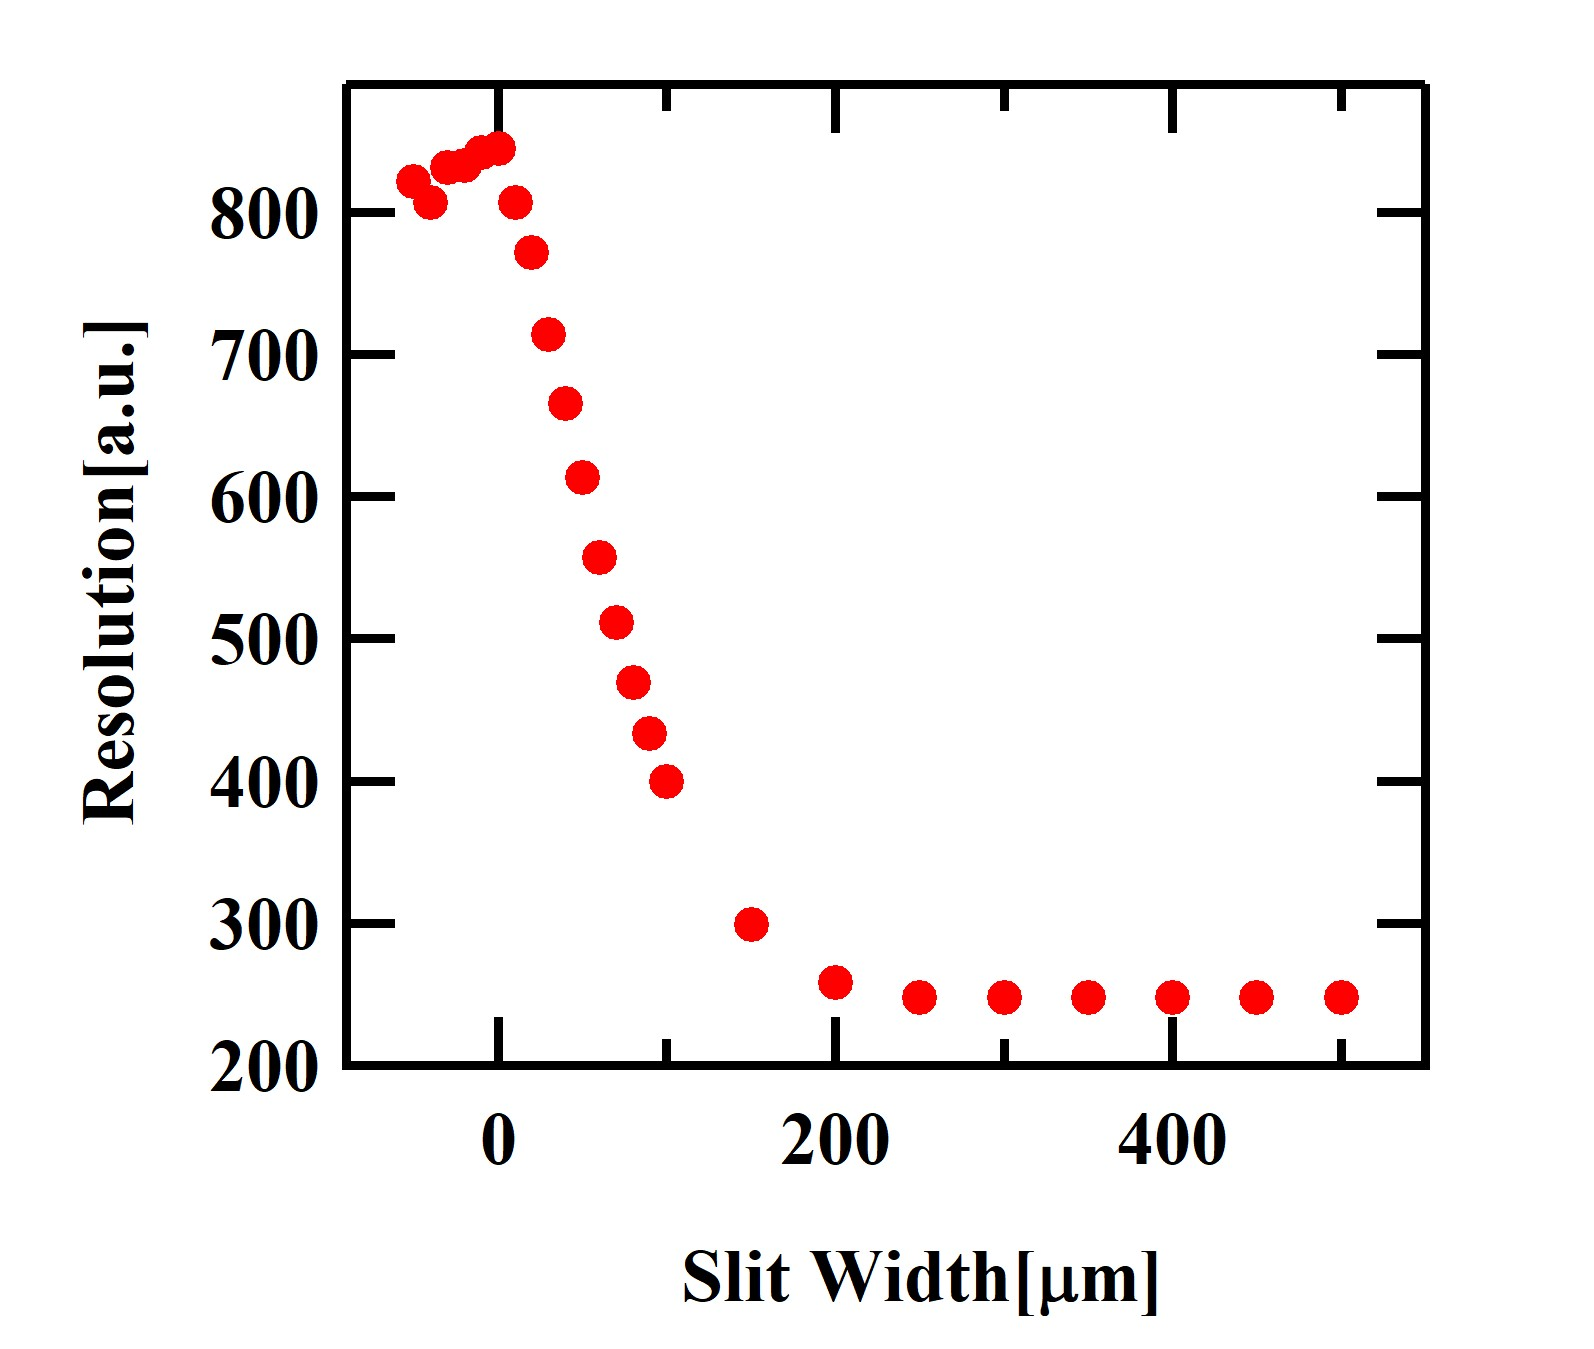
\includegraphics[clip,width=9cm]{start1_300Resolution.jpg}
        \caption{300 g/mmの回折格子における分光器のスリット幅と分解能の関係.}
        \label{fig_300resolution1}
       \end{figure}

       縦軸は分解能、横軸はスリット幅である。スリット幅が0 $\upmu$mから広くなるにつれて、分解能が下がっていることが分かる。つまり、スペクトル幅だけを考えるのならば、スリット幅が狭ければ狭いほど、実験データの精度が良くなる。
       しかし、スリット幅が狭くなってゆくと、スリットから入射される光の強度にも変化が現れる。スリット幅と入射光強度の関係を図\ref{fig_300Int1}に示す。

       \newpage
       \begin{figure}[ht]
        \centering
        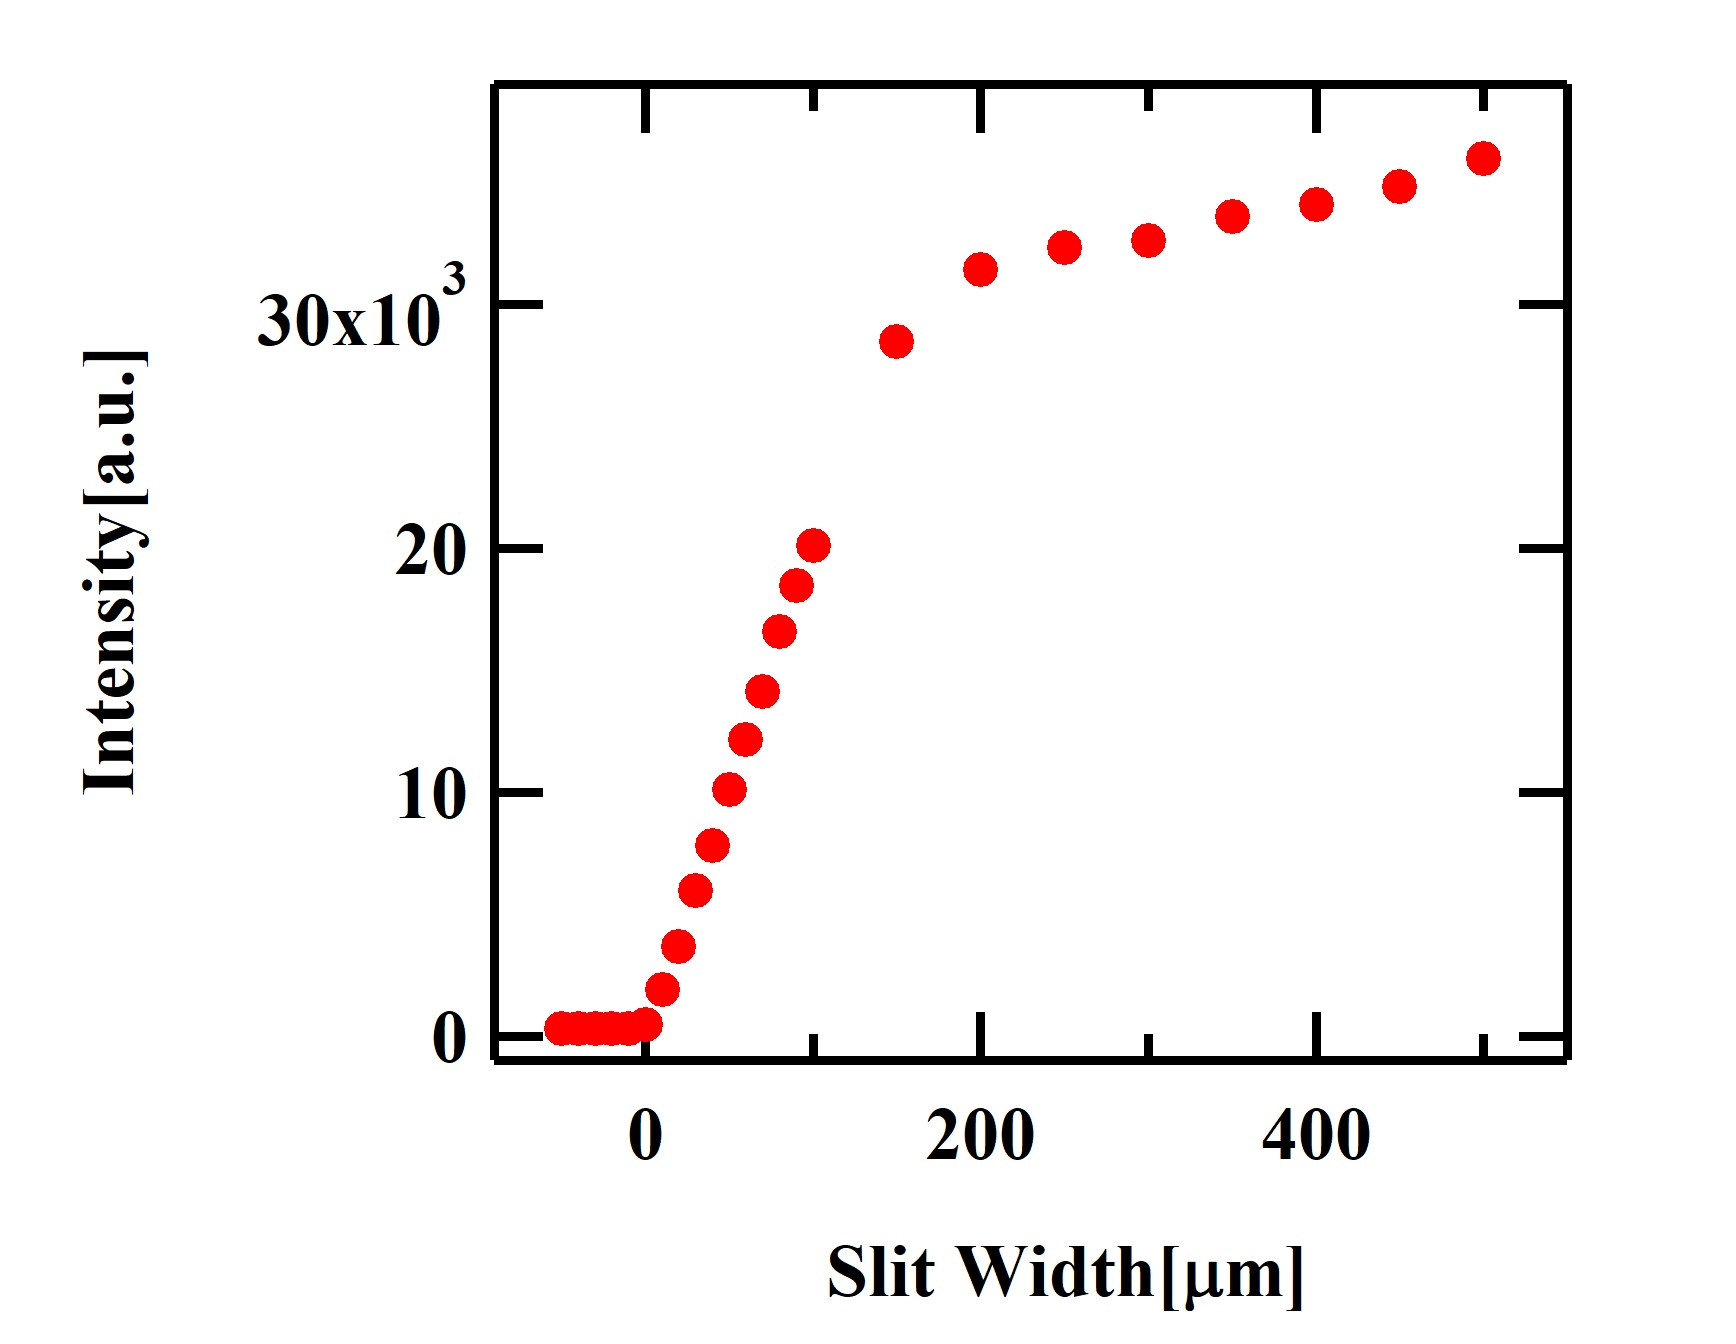
\includegraphics[clip,width=9cm]{start1_300Int.jpg}
        \caption{300 g/mmの回折格子における分光器のスリット幅と入射光強度の関係.}
        \label{fig_300Int1}
       \end{figure}


       縦軸は入射光強度、横軸はスリット幅である。スリット幅が大きいほど強い光が入射していることが分かる。スリット幅が200 $\upmu$mより広い部分で、入射光強度の増加量が減っている。これは、光ファイバーのコアの幅が有限であるためである。スリット幅がファイバーのコアの直径より狭いうちは、スリット幅に比例して入射光強度が大きくなるが、コアの直径を超えた時点で、入射光強度はコアの直径によって定まってしまうため、スリット幅では入射光強度を調整できなくなる。\\
       入射光強度が大きいほど、ノイズの影響が小さくなるので、入射光強度だけを考えるのならば、スリット幅が広ければ広いほど実験の精度が良くなる。したがって、実験を行う際はスペクトル幅と入射光強度の兼ね合いでスリット幅を決定する必要がある。ただし、スリットからの入射光強度は、スリット幅以外での調整が可能なため、スペクトル幅を重視し、なるだけ狭いスリット幅で実験を行うべきである。

       \newpage

 \item 1200 g/mmの回折格子を用いた測定


       1200 g/mmの回折格子を用いた時の、分光器のスリット幅とスペクトル幅の関係を図\ref{fig_1200spectrum1}に示す。

       \begin{figure}[ht]
        \centering
        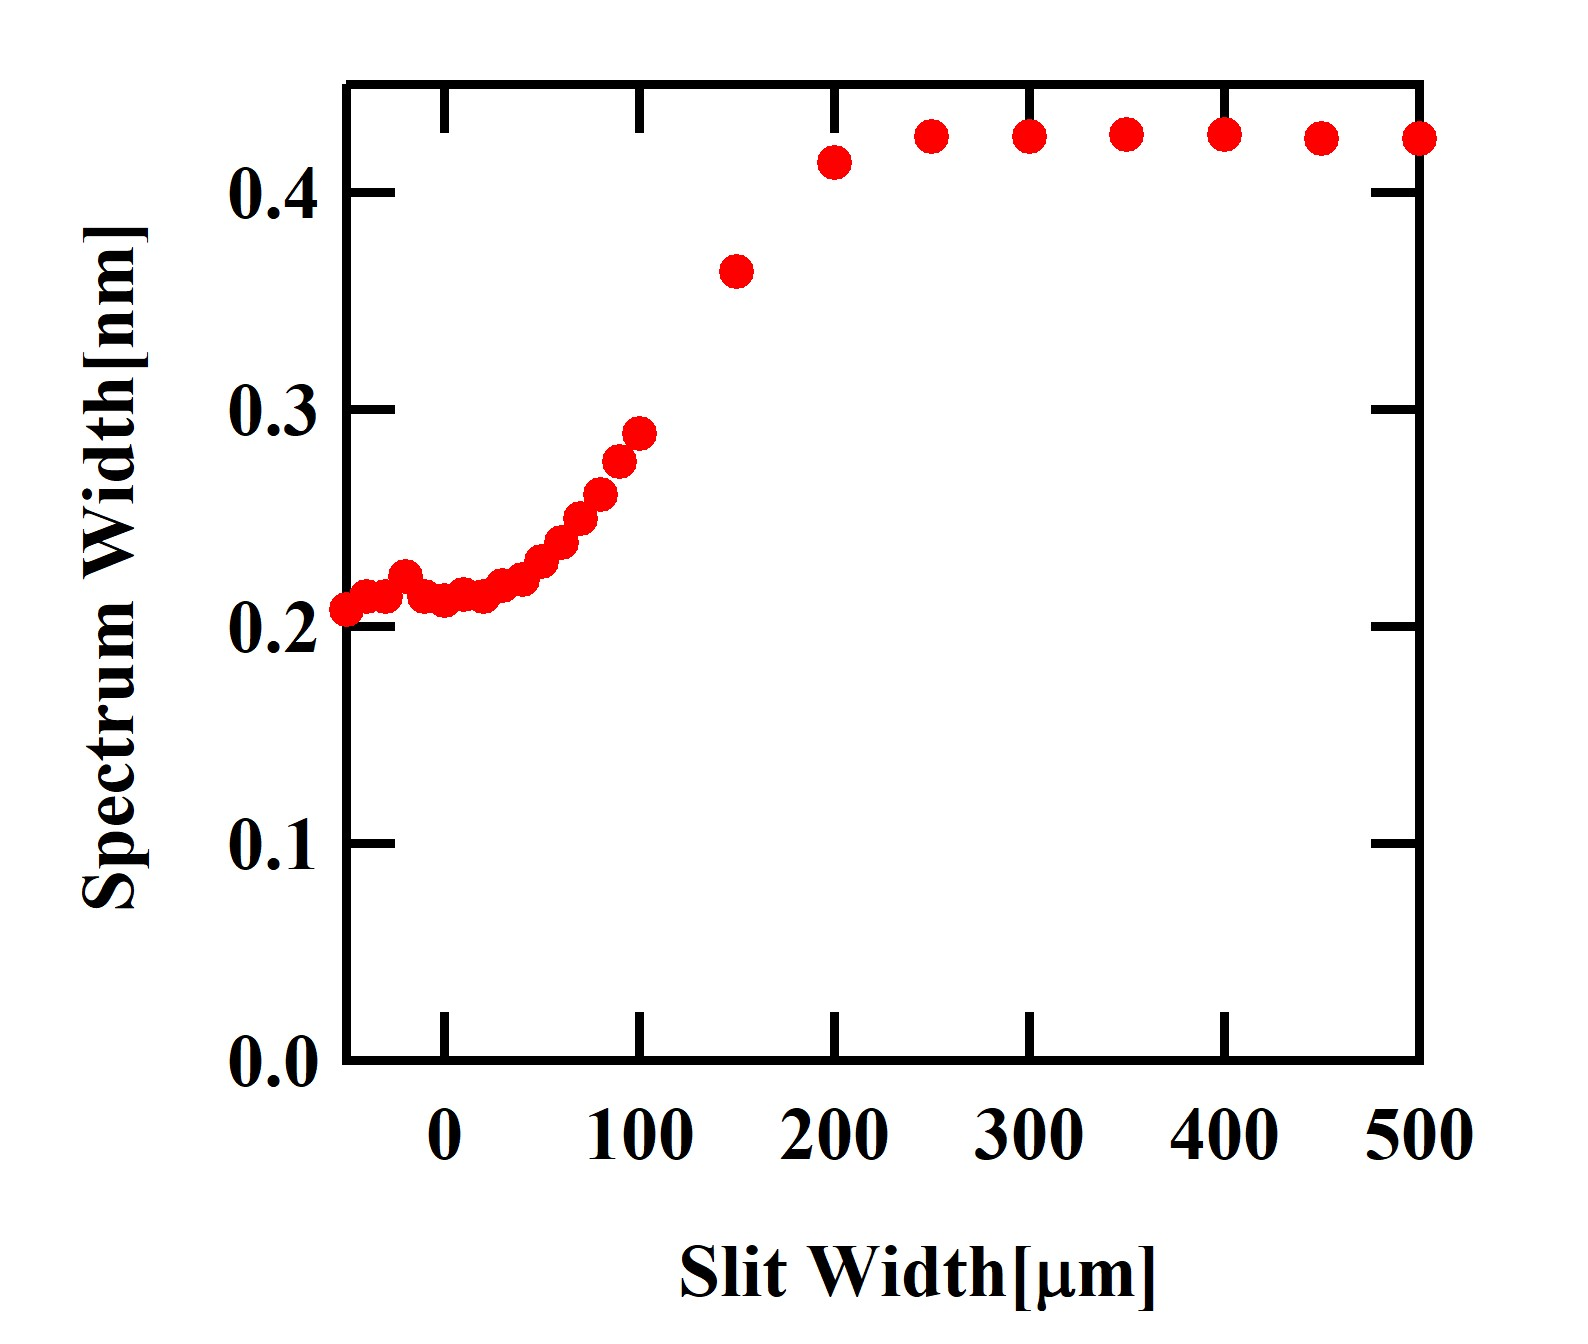
\includegraphics[clip,width=9cm]{start1_1200Spectrum.jpg}
        \caption{1200 g/mmの回折格子における分光器のスリット幅とスペクトル幅の関係.}
        \label{fig_1200spectrum1}
       \end{figure}


       縦軸は水銀灯の発光スペクトルのスペクトルの幅、横軸はスリット幅である。300 g/mmの時と同様、スリット幅が大きくなると、スペクトル幅が広がっているのがわかる。スリット幅と分解能の関係を図\ref{fig_1200_resolution1}に、スリット幅と入射光強度の関係を図\ref{fig_1200_Int1}に示す。

       \begin{figure}[t]
        \centering
        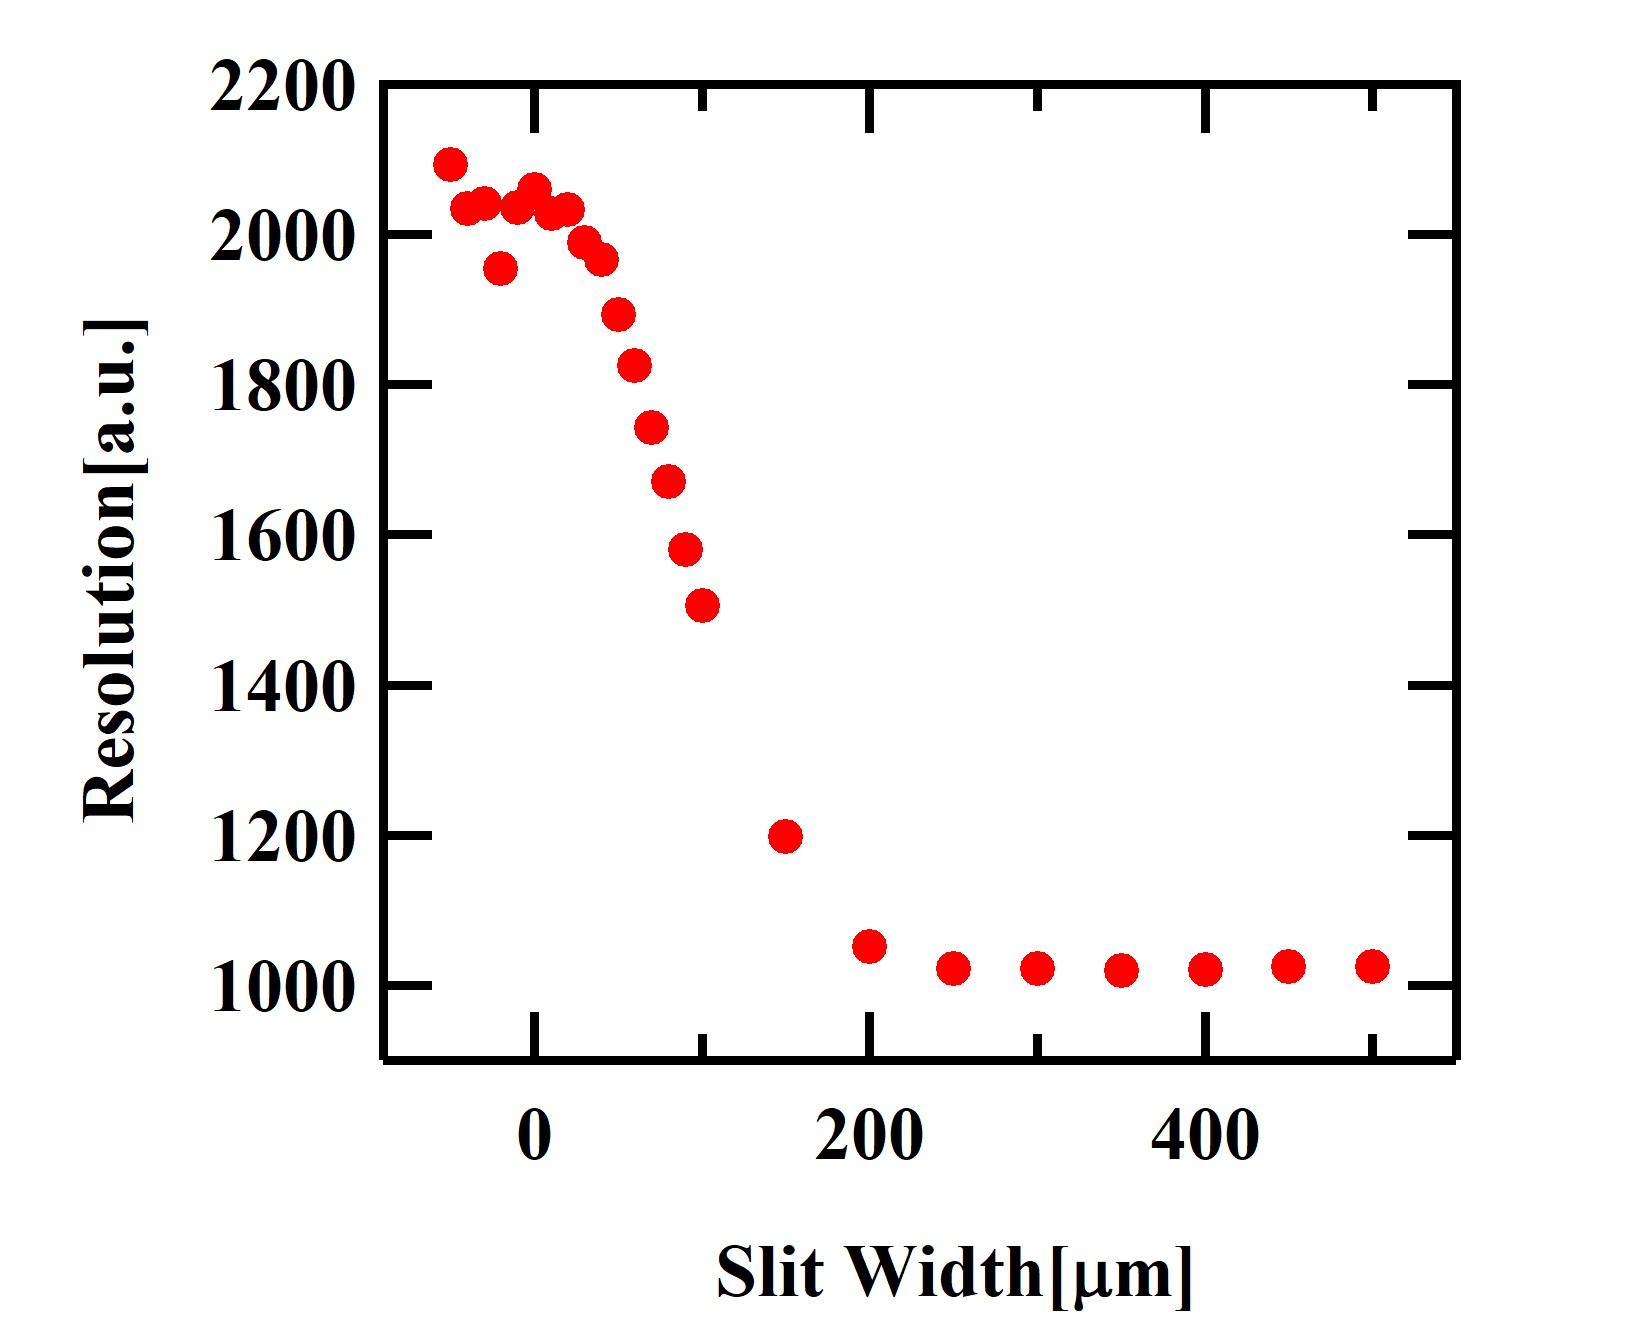
\includegraphics[clip,width=9cm]{start1_1200Resolution.jpg}
        \caption{1200 g/mmの回折格子における分光器のスリット幅と分解能の関係.}
        \label{fig_1200_resolution1}
       \end{figure}

       \newpage

       \begin{figure}[ht]
        \centering
        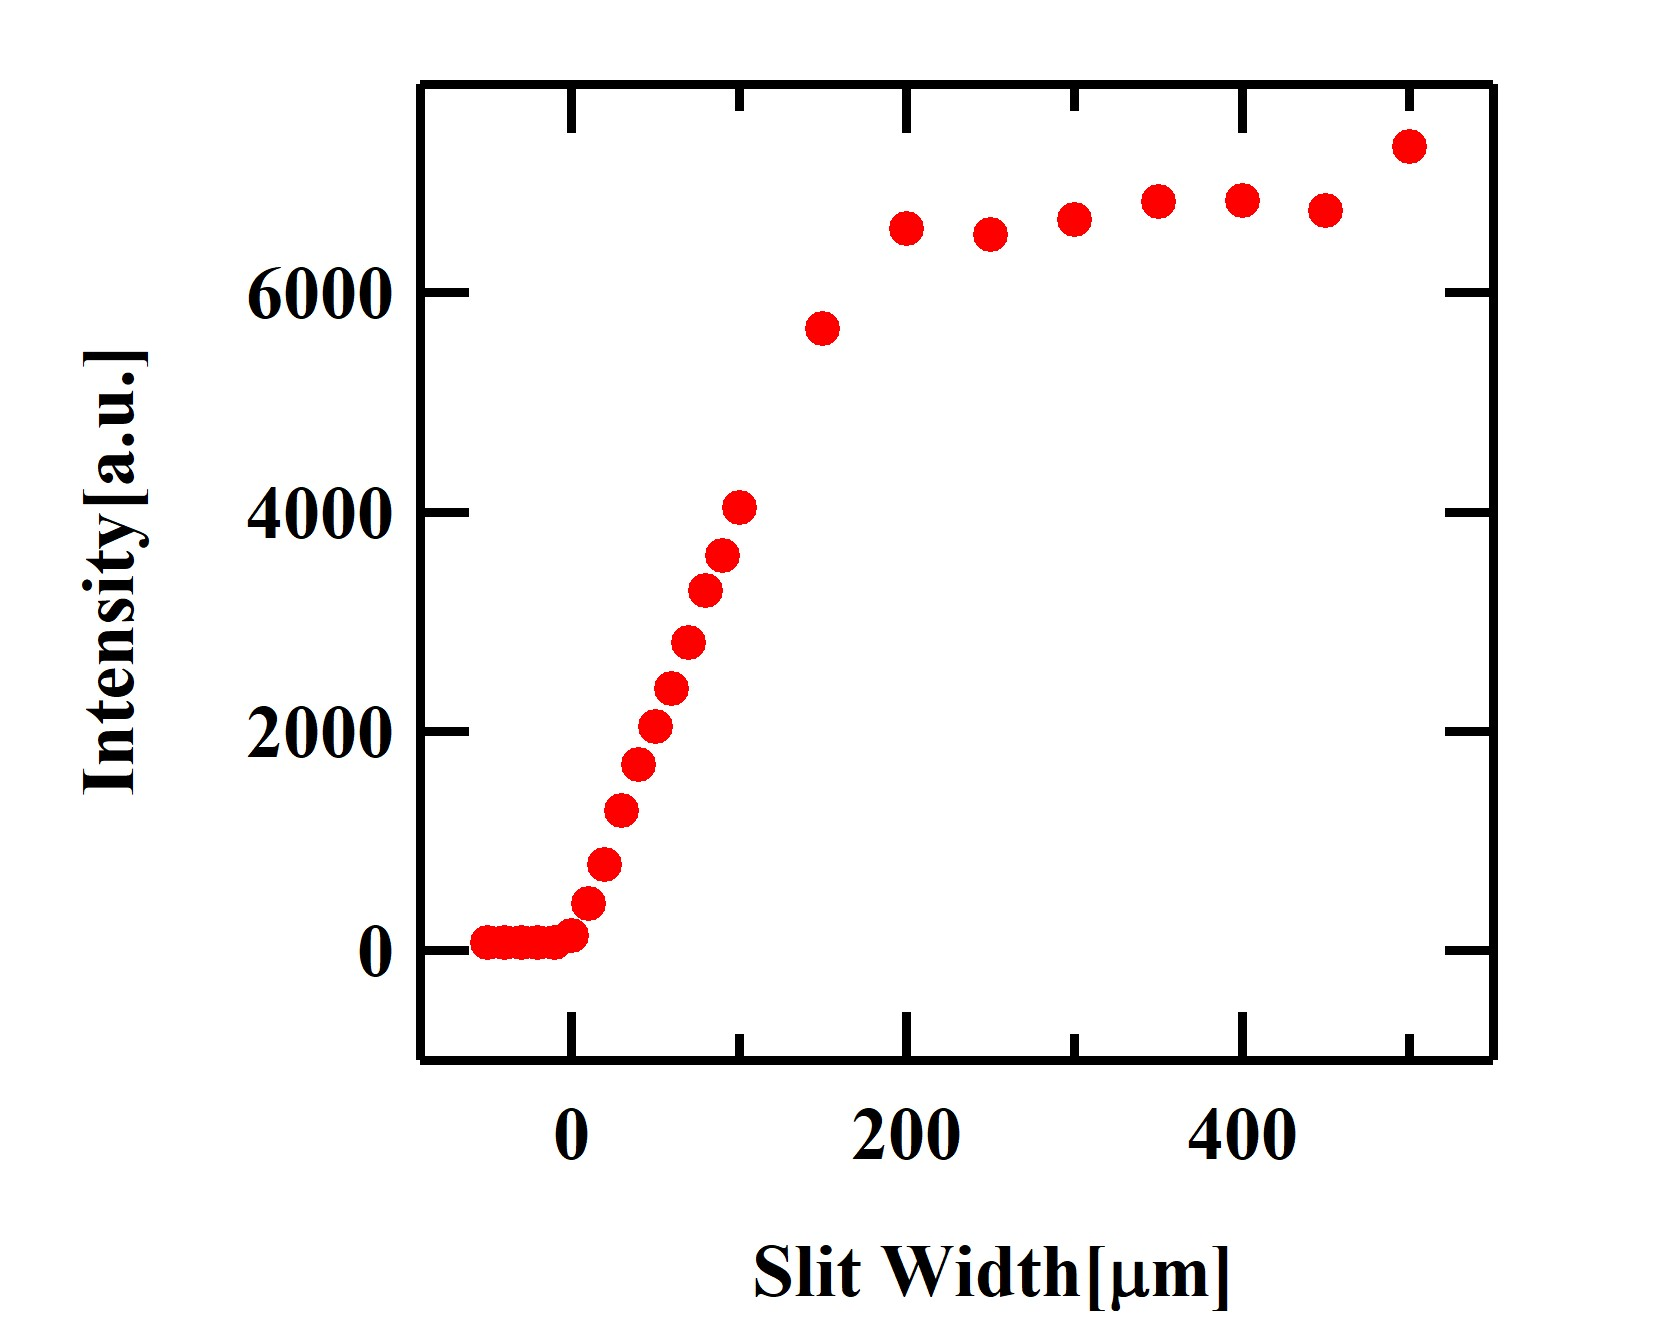
\includegraphics[clip,width=9cm]{start1_1200Intensity.jpg}
        \caption{1200 g/mmの回折格子における、分光器のスリット幅と入射光強度の関係.}
        \label{fig_1200_Int1}
       \end{figure}

       図\ref{fig_1200_resolution1}の縦軸は分解能、横軸はスリット幅である。図\ref{fig_1200_Int1}の縦軸は入射光強度、横軸はスリット幅である。これらも300 g/mmの時と同様、スリット幅が0 $\upmu$mから広くなるにつれて、分解能が下がっていること、スリット幅が大きいほど強い光が入射していることが分かる。この結果を用いて、単位長さ当たりのグレーティングの数と分解能の関係を考える。

       \newpage
 \item 2つの回折格子の比較

       2つの回折格子における、スリット幅と分解能の関係を図\ref{fig_resolution1}に示す。

       \begin{figure}[ht]
        \centering
        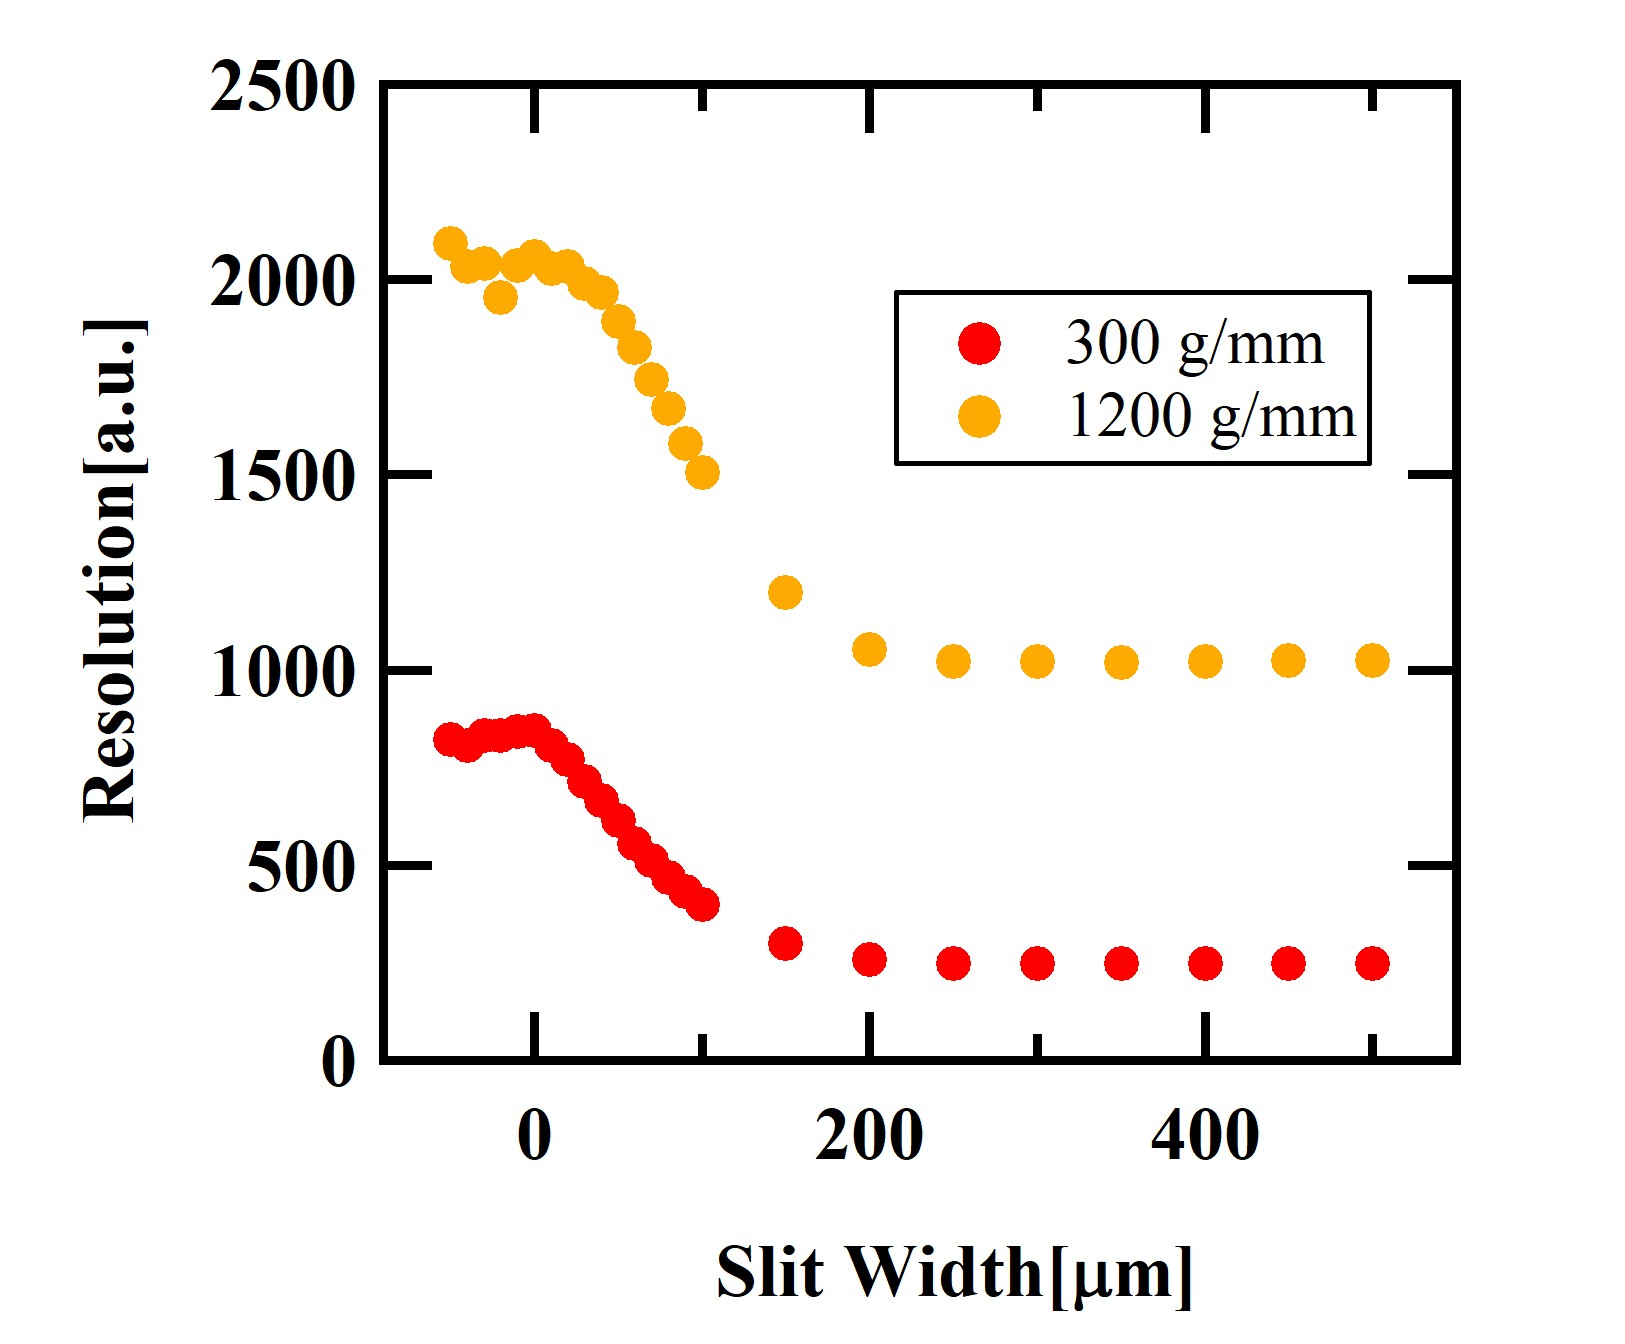
\includegraphics[clip,width=9cm]{start1_Resolution.jpg}
        \caption{2つの回折格子における分光器のスリット幅と分解能の関係.}
        \label{fig_resolution1}
       \end{figure}

       縦軸は分解能、横軸はスリット幅である。いずれのスリット幅においても、300 g/mmの回折格子よりも、1200 g/mmの回折格子のほうが分解能が高い。分解能$R$は$R=mN$でも表される。$N$は光が当たっているグレーティングの数なので、1200 g/mmの回折格子を用いた時は、300 g/mmの回折格子を用いた時より4倍分解能が高い。図\ref{fig_resolution1}をみると、スリット幅が150 $\upmu$mより広いときに、1200 g/mmの分解能が300 g/mmの4倍になっている。そのため、今回の実験環境では、スリット幅が150 $\upmu$mより狭いときは入射光強度が不足していると考えられる。%考察

\end{enumerate}%箇条書きここまで

\newpage

\subsection{実験2. 半導体試料の発光スペクトルの励起光強度依存性}
\subsubsection{実験2.1. CdSの発光スペクトルの励起光強度依存性}

室温のCdSに波長450 nmのレーザーを照射して得られた発光スペクトルを測定した。結果を図\ref{fig_cds_rt_spec1}に示す。実験2.1.では、得られたデータに対し分光器とフィルターの感度補正を行った。

\begin{figure}[ht]
 \centering
 \begin{tabular}{c}

  \begin{minipage}{0.5\hsize}

   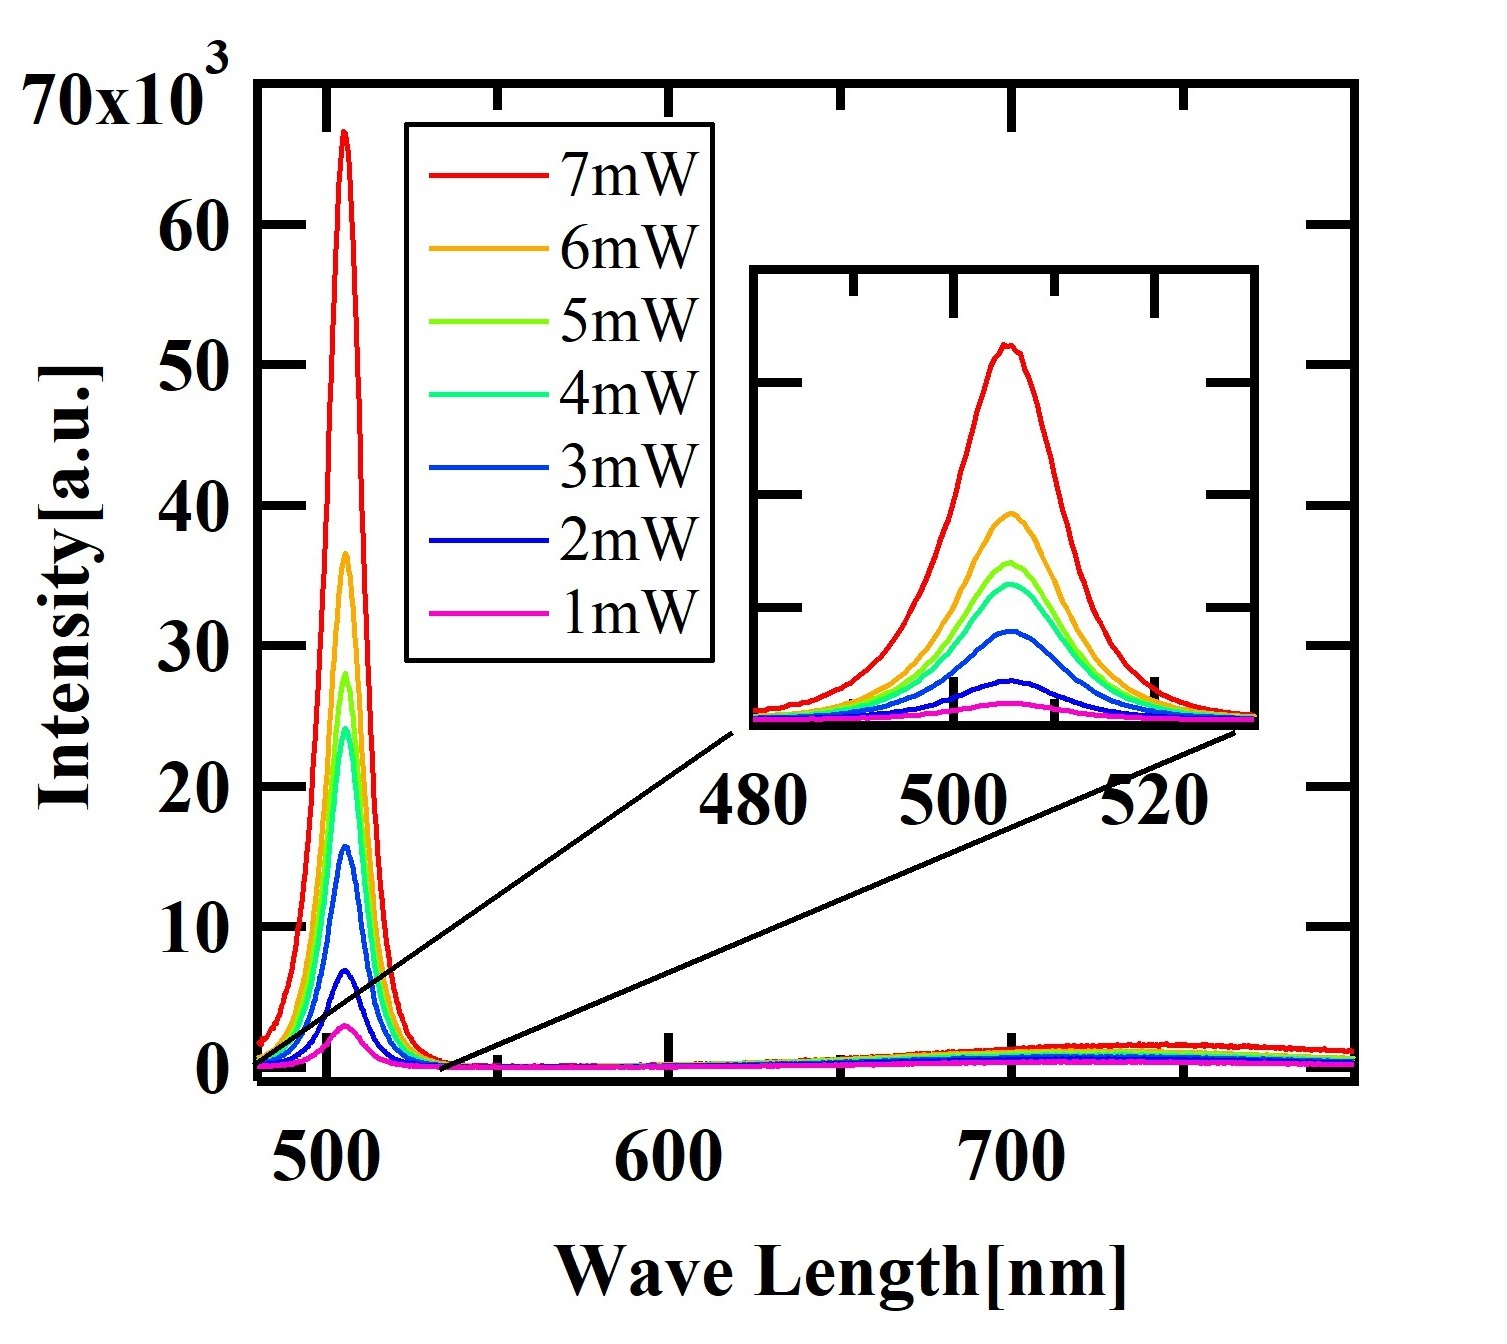
\includegraphics[clip,width=8cm]{start2_CdS_rt_Spectrum_wav.jpg}
  \end{minipage}

  \begin{minipage}{0.5\hsize}
   \centering
   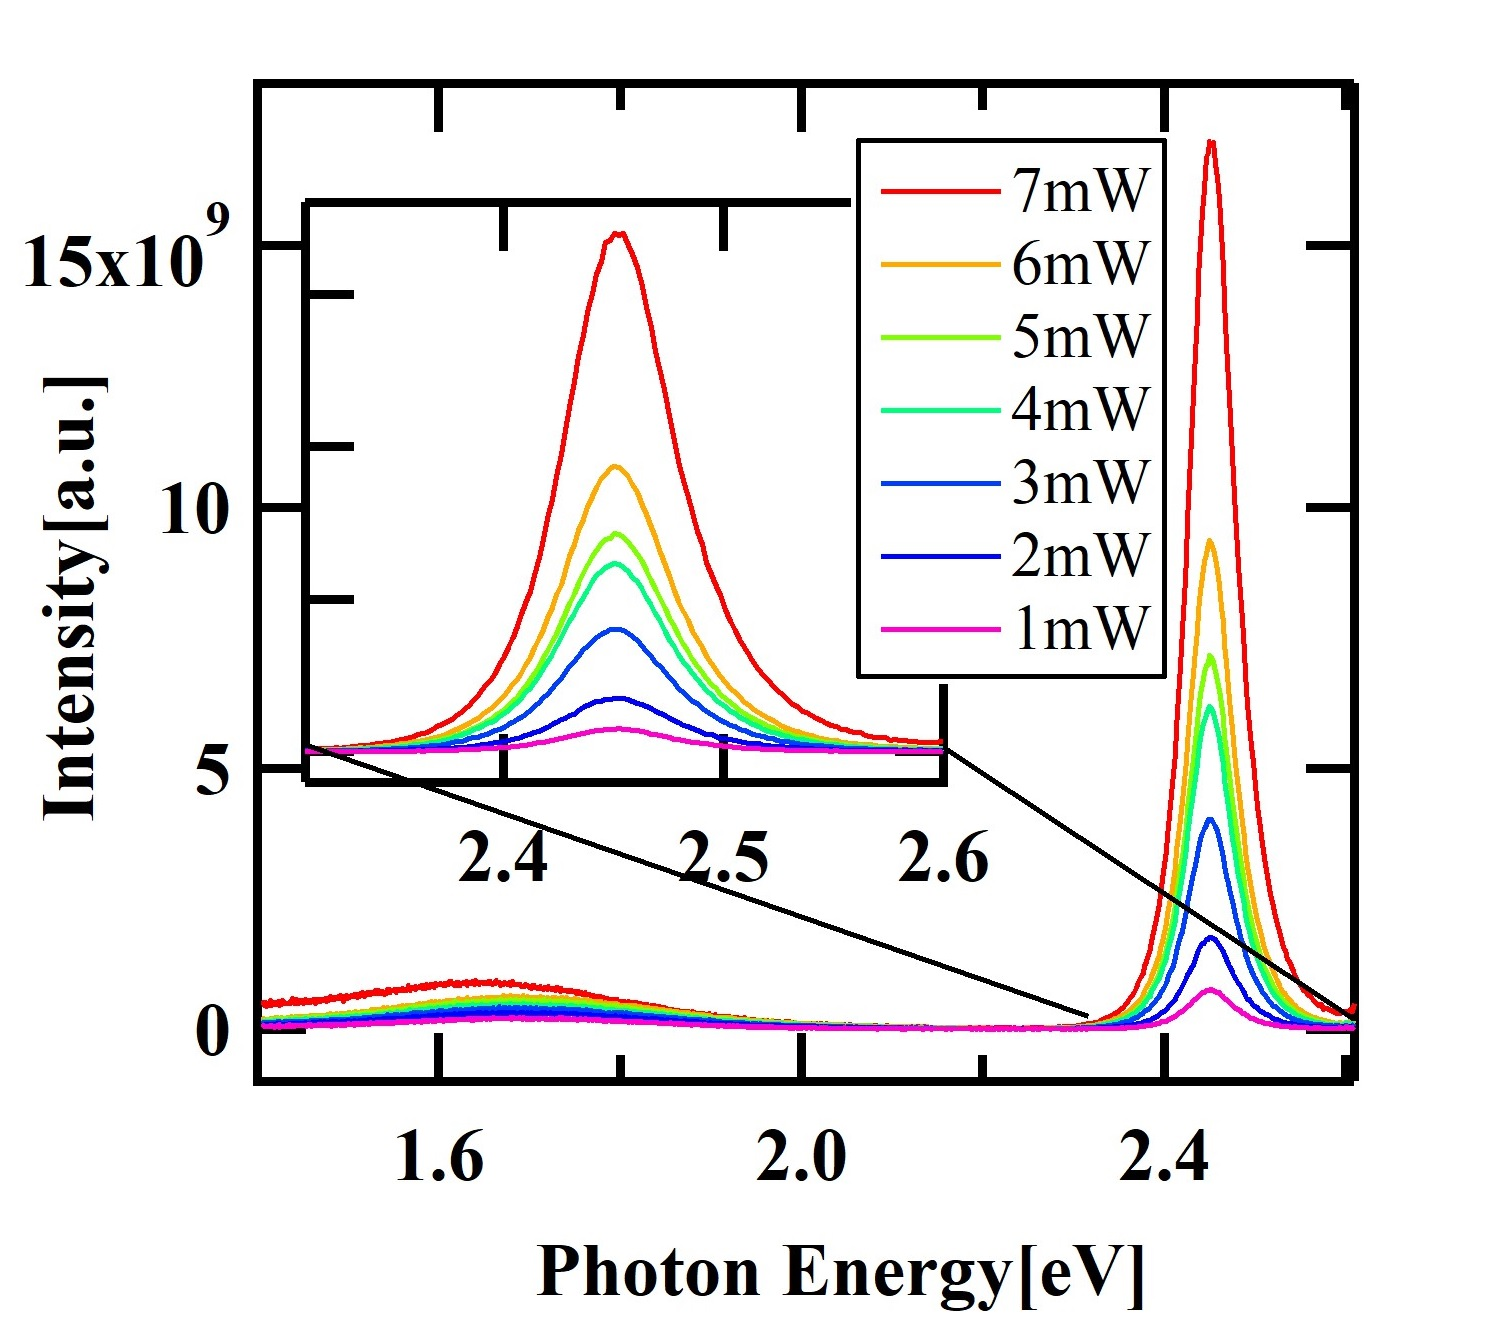
\includegraphics[clip,width=8cm]{start2_CdS_rt_Spectrum_eV.jpg}
  \end{minipage}
 \end{tabular}
 \caption{室温のCdSにおける発光スペクトル.}
 \label{fig_cds_rt_spec1}

\end{figure}

縦軸はどちらも発光強度である。左図の横軸は波長、右図の横軸は光子エネルギーである。波長域480 nmから530 nmにピークが見られた。
%
%\begin{figure}[ht]
%	\centering
%	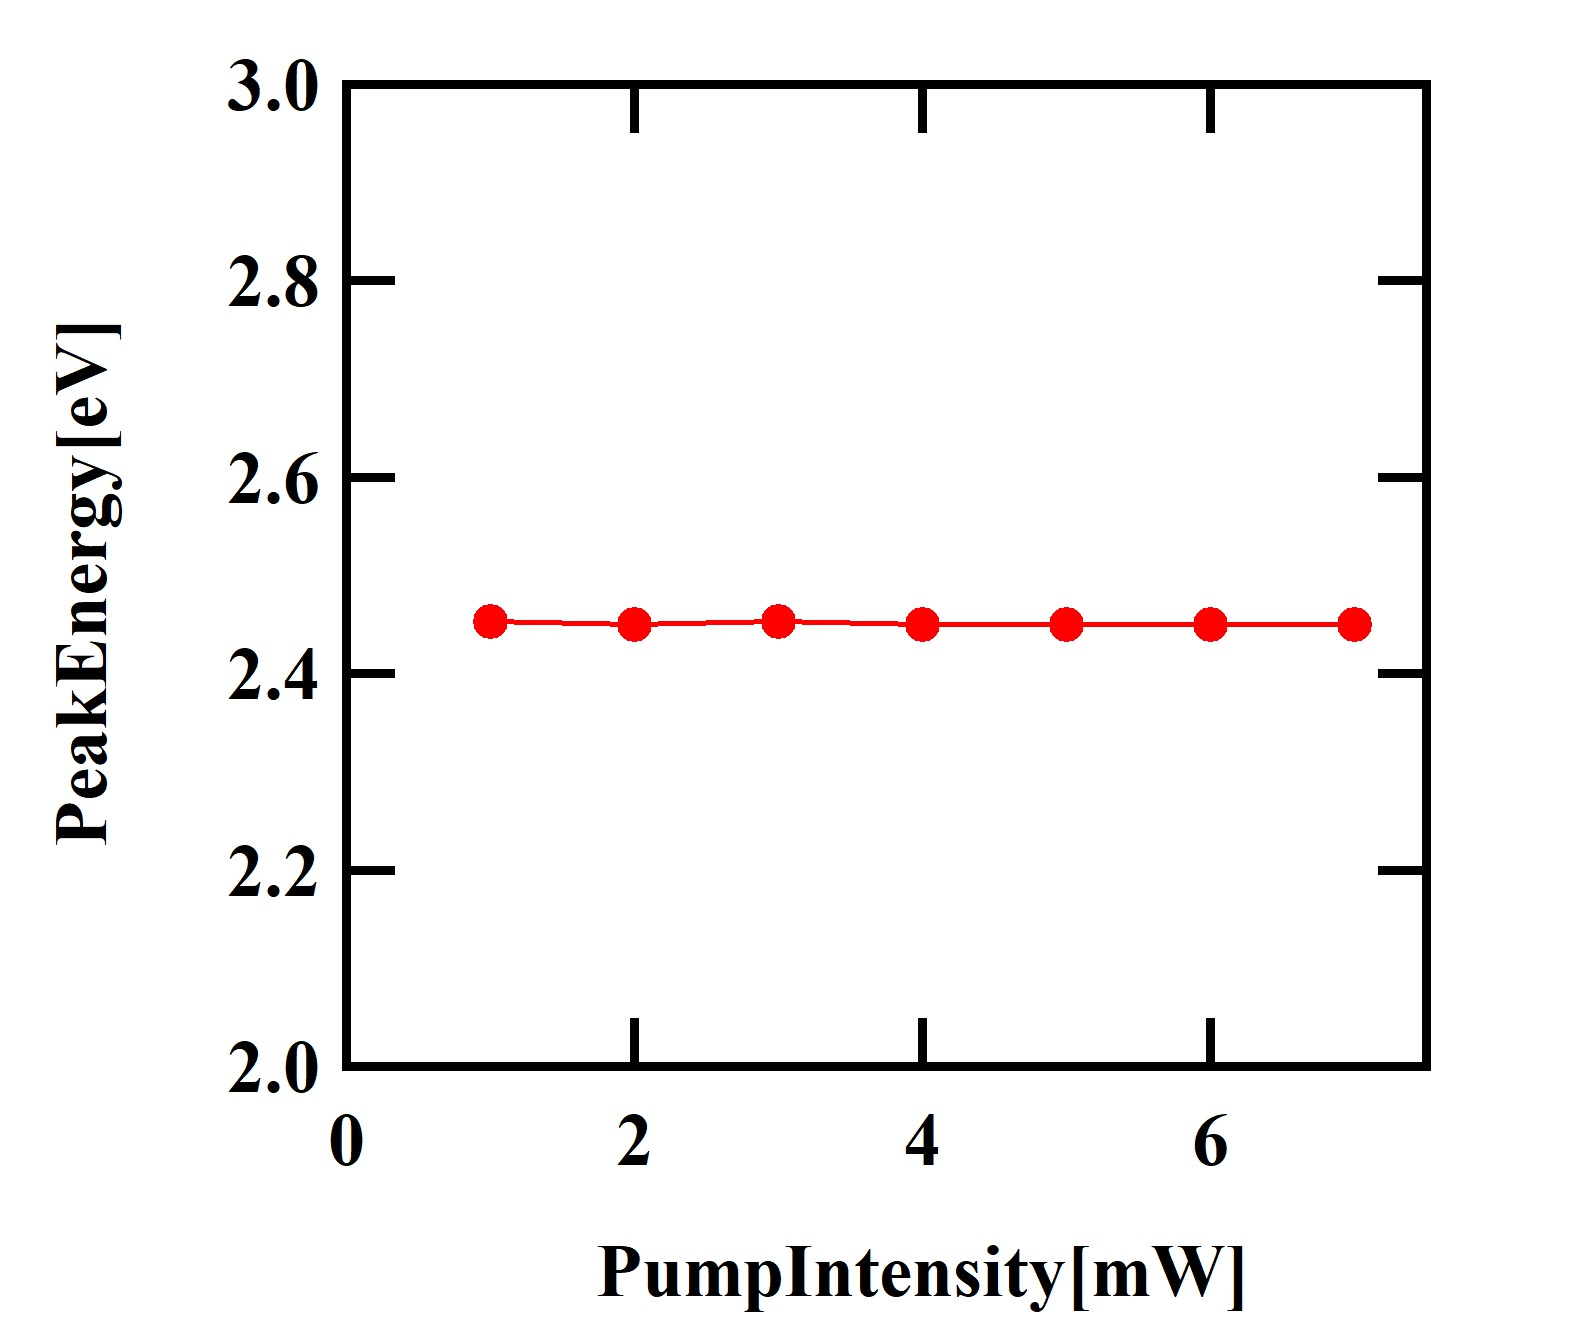
\includegraphics[clip,width=9cm]{start2_CdS_rt_Peak.jpg}
%	\caption{室温のCdSの、エネルギー域2.3 eVから2.6 eVの発光スペクトルにおける励起光強度とピークエネルギーの関係.}
%	\label{fig_cds_rt_peak1}
%\end{figure}

いずれの励起光強度においても、波長505 nm(エネルギー換算で2.45 eV)付近にピークがある。
室温におけるCdSのエネルギーギャップは2.42 eVである\cite{gapE}が、図\ref{fig_cds_rt_spec1}から、それよりも低いエネルギーにおいても発光をしていることが読み取れる。バンド間の幅が小さくなっていることから、励起子が発生していることがうかがえる。CdS中の励起子の束縛エネルギーは28 meVである\cite{exciton}。室温における熱エネルギー$\mathrm{k_{B}}T$はおおよそ26 meVと励起子の束縛エネルギーより低いため、室温のCdS中に励起子は存在可能である。光子エネルギーはバンドギャップエネルギーよりも束縛エネルギーの分だけ小さくなるため、励起子準位からの発光の光子エネルギーは2.36 eV程度である。すなわち、図\ref{fig_cds_rt_spec1}の発光スペクトルは、CdSの励起子からの発光と、バンド間発光の両方が合わさったものである。
励起光強度が大きくなるにつれて、発光強度が大きくなっていることが読み取れる。励起光強度の大きさと発光強度の大きさの関係を図\ref{fig_cds_rt_int1}に示す。

\begin{figure}[ht]
 \centering
 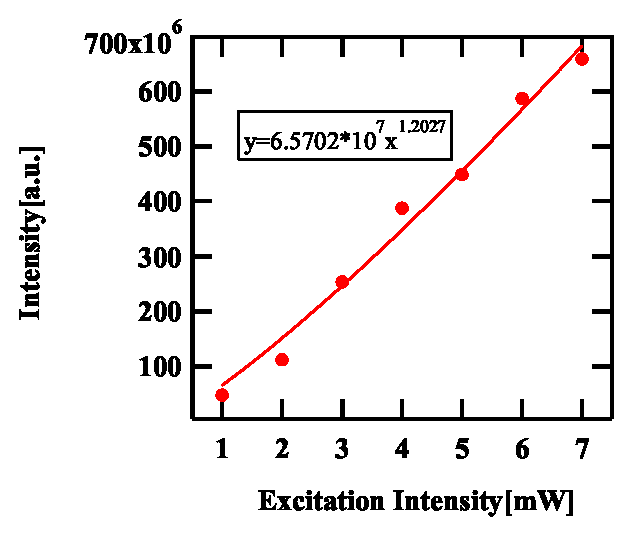
\includegraphics[clip,width=8.5cm]{start2_CdS_rt_Int.eps}
 \caption{室温のCdSの発光スペクトルにおける励起光強度と発光強度の関係.}
 \label{fig_cds_rt_int1}
\end{figure}

\newpage
縦軸は発光強度、横軸は励起光強度である。バンド間発光の場合、励起光強度が増加すると、増えた分だけ励起される電子も増加する。そのため、発光強度は励起光強度に比例する。発光強度の励起光強度依存性を議論するため、発光強度を$y$、励起光強度を$x$としたとき、$y=\mathrm{A}x^{B}$の形で表す。
バンド間発光のみが発生しているときの発光強度は励起光強度に比例するため、$B$の値は1である。励起子が存在するとき、励起子どうしの衝突が発生する。衝突の頻度が顕著な時、励起子分子が形成される。励起子分子と励起子が準熱平衡状態の時、励起光強度が低い領域では、励起子分子発光強度は励起光強度の自乗に比例するため、$B$の値は2になる。室温のCdSでは、熱エネルギーに対して、励起子の束縛エネルギーは大きくない。そのため、衝突の頻度が少なく、励起子分子の形成は少ない。そのため、$B$の値が1に近い値になっている。

%ここからCdSの不純物
図\ref{fig_cds_rt_spec1}の発光スペクトルのうち、波長域580 nmから880 nmの範囲を拡大したものを図\ref{fig_cds_imp_spec1}に示す。

\newpage
\begin{figure}[ht]
 \centering
 \begin{tabular}{c}

  \begin{minipage}{0.5\hsize}

   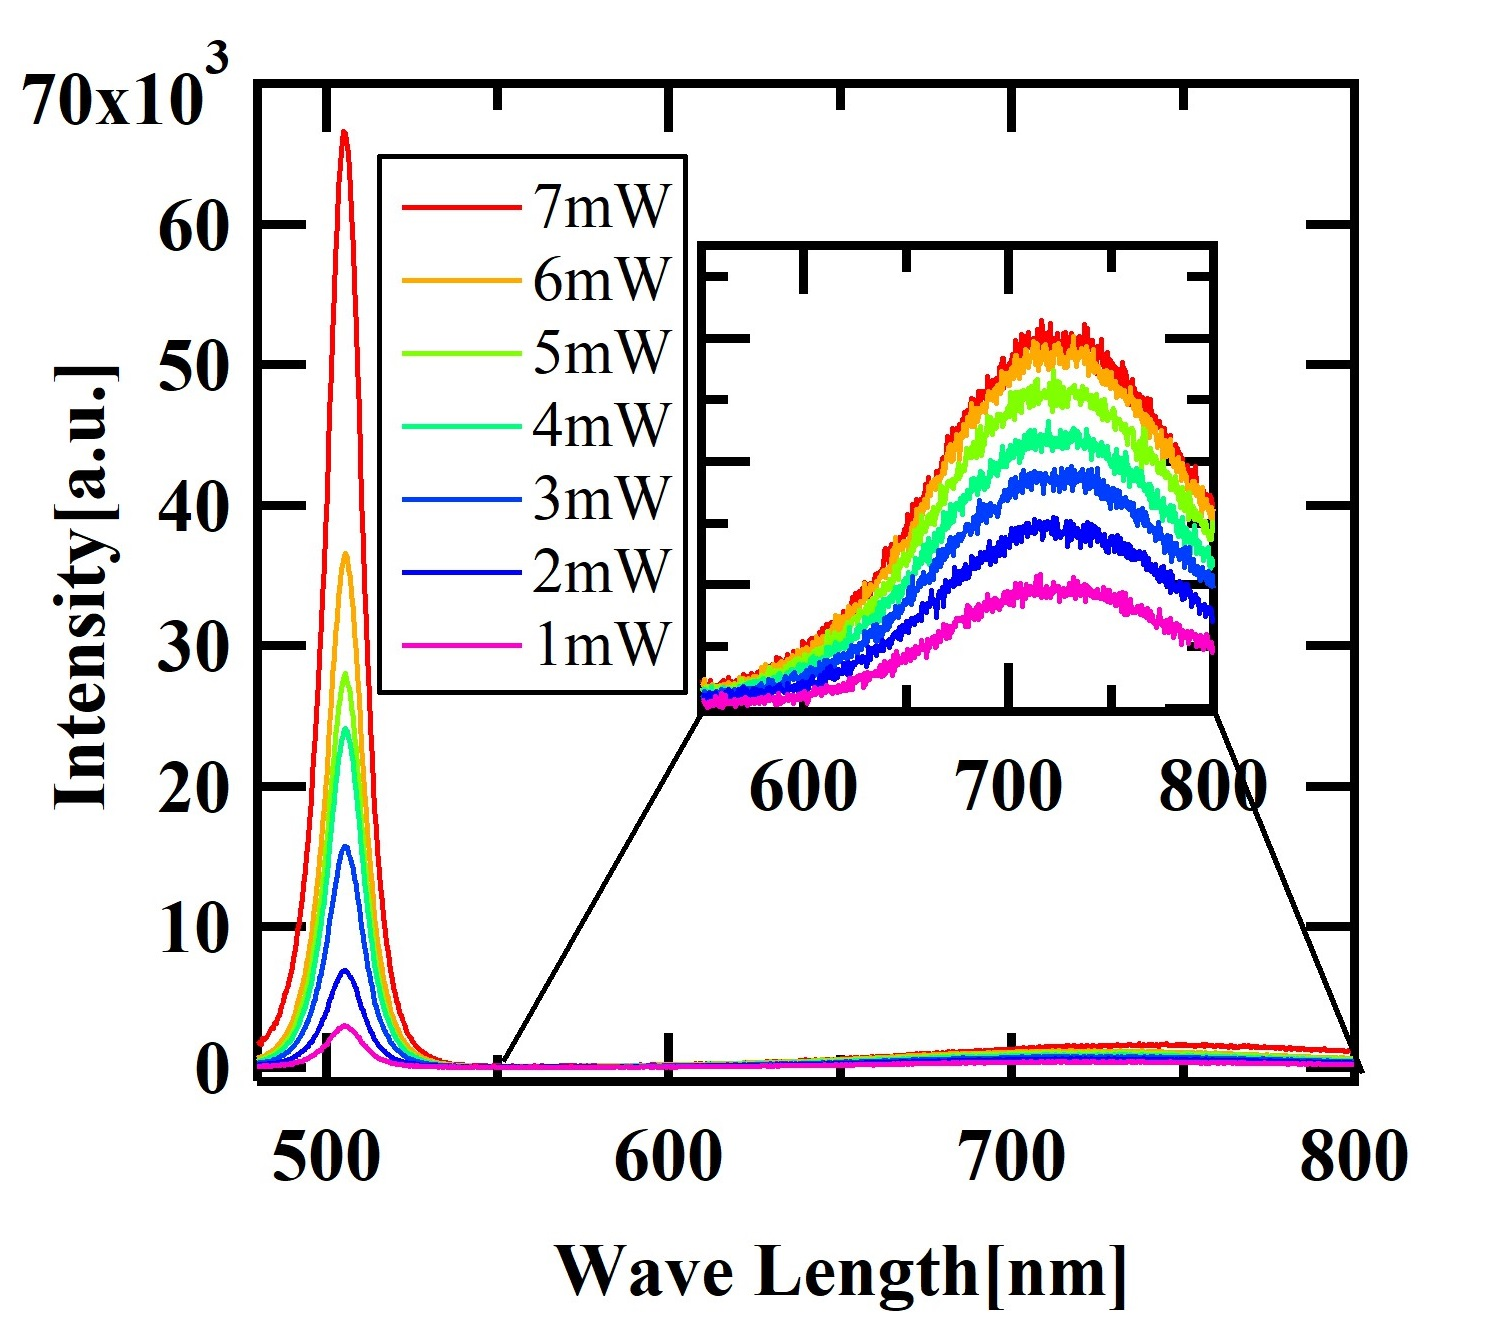
\includegraphics[clip,width=8cm]{start2_CdS_imp_Spectrum_wav.jpg}
  \end{minipage}

  \begin{minipage}{0.5\hsize}
   \centering
   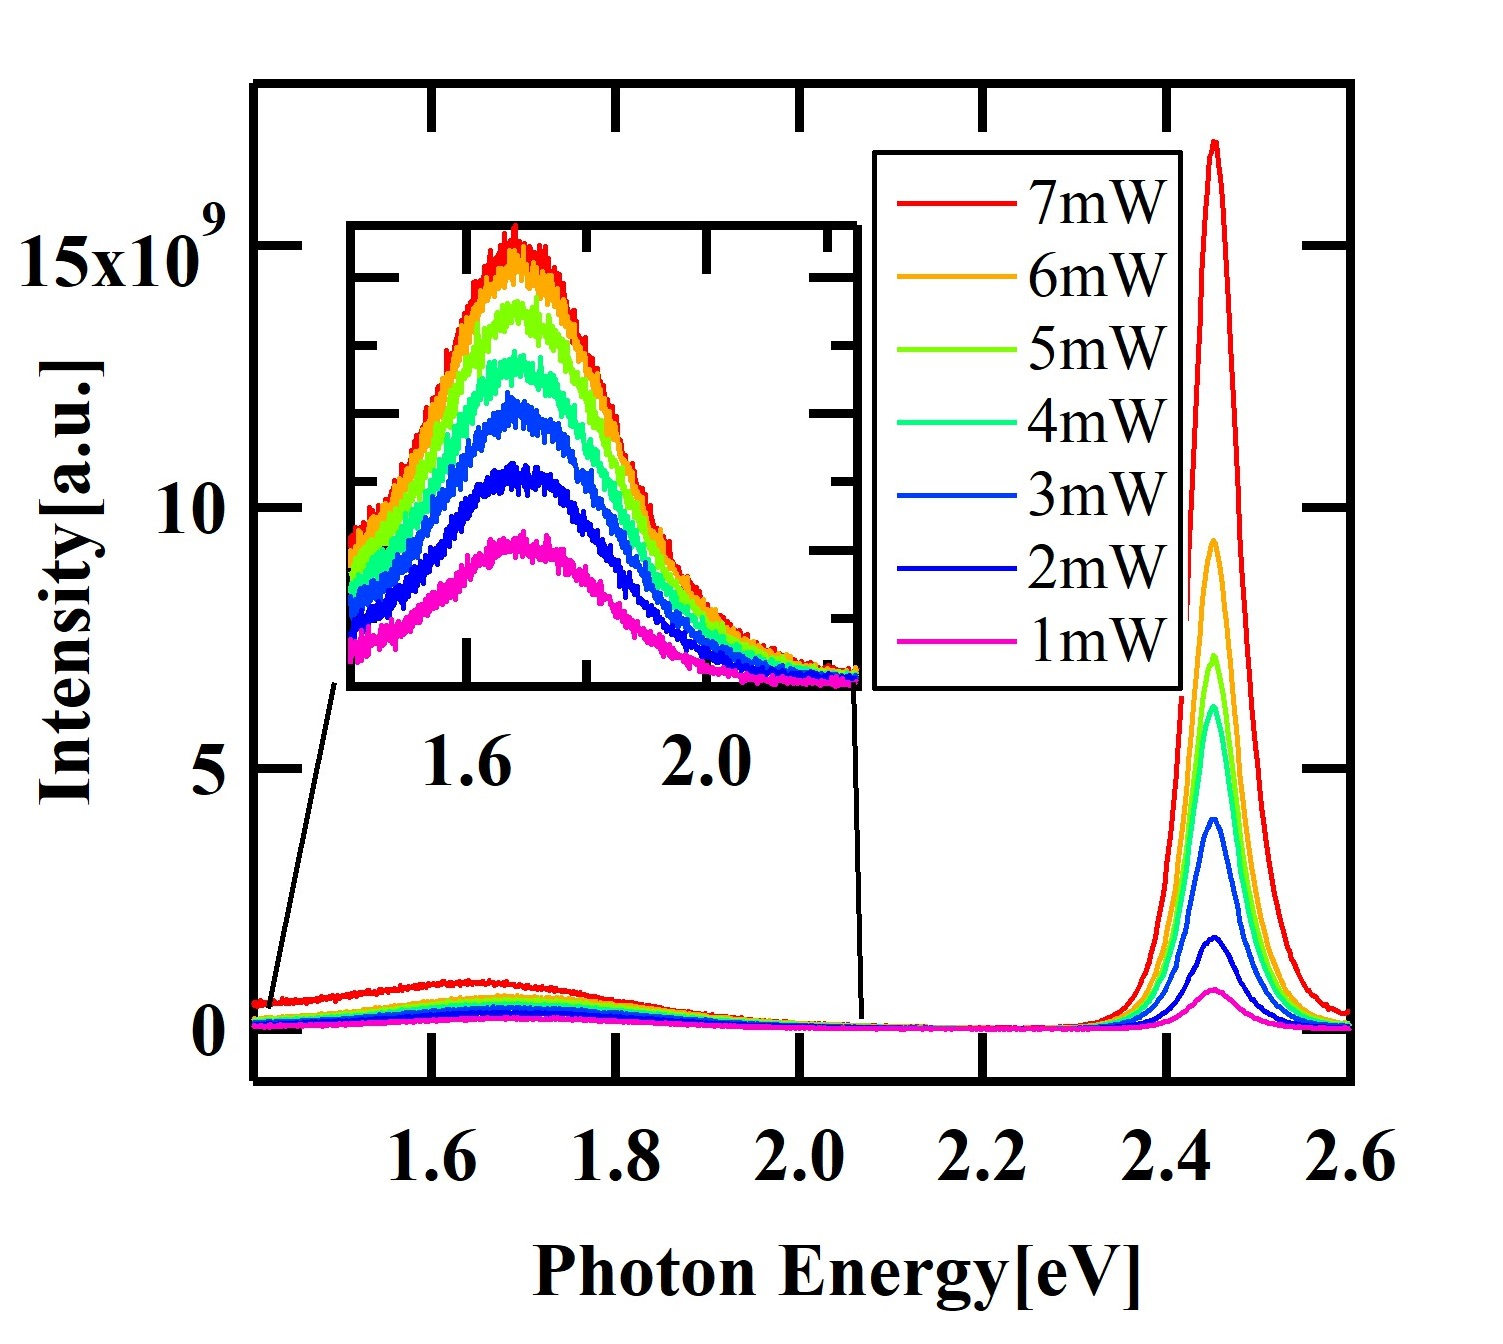
\includegraphics[clip,width=8cm]{start2_CdS_imp_Spectrum_eV.jpg}
  \end{minipage}
 \end{tabular}
 \caption{室温のCdSにおける発光スペクトル.}
 \label{fig_cds_imp_spec1}

\end{figure}

縦軸はどちらも発光強度である。左図の横軸は波長、右図の横軸は光子エネルギーである。いずれの励起光強度においても、波長730 nm(エネルギー換算で1.69 eV)付近にピークがある。このスペクトルの裾の引きはじめは、測定範囲の都合から読み取ることができなかった。図\ref{fig_cds_rt_spec1}に比べて曲線が荒いのは、発光強度が十分に大きくないためである。
%各励起光強度におけるピークエネルギーを図\ref{fig_cds_imp_peak1}に示す。

%\begin{figure}[ht]
%	\centering
%	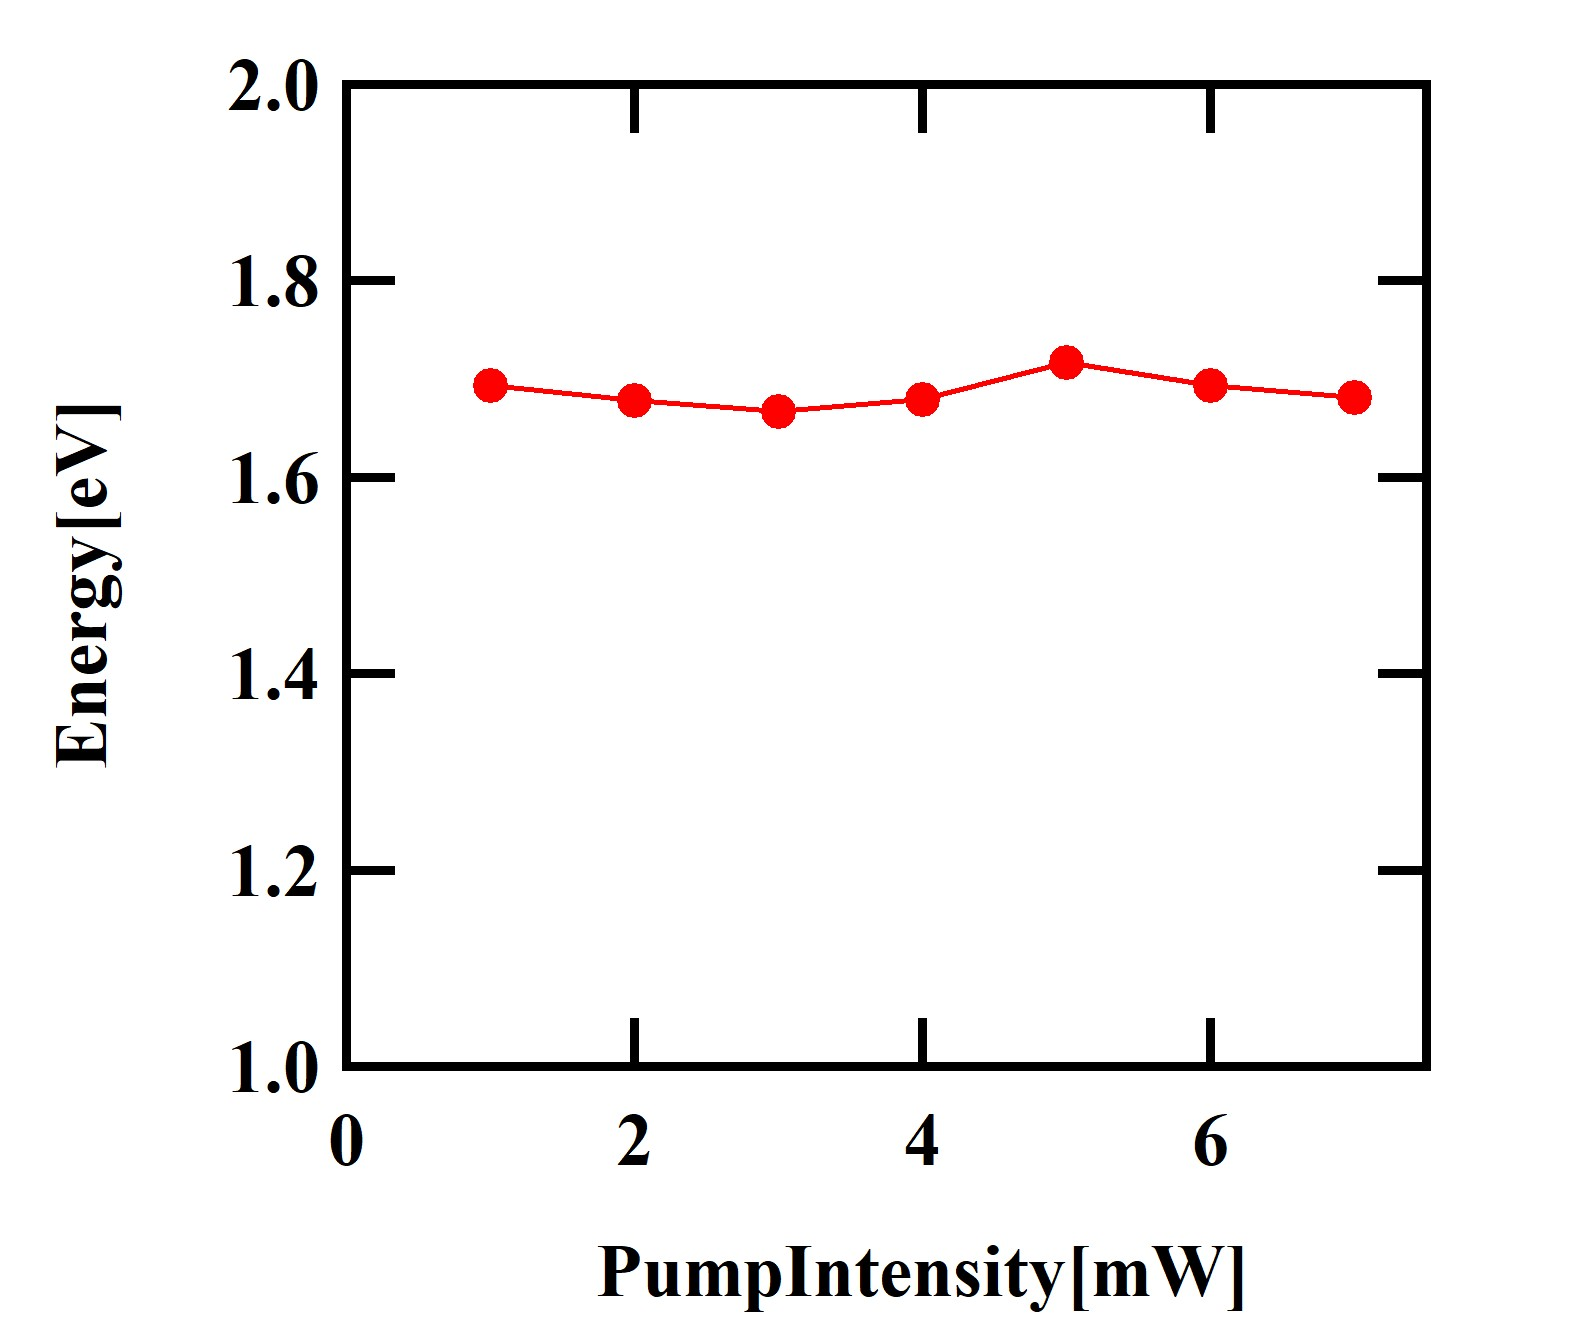
\includegraphics[clip,width=8.5cm]{start2_CdS_imp_Peak.jpg}
%	\caption{室温のCdSの、エネルギー域1.4 eVから2.3 eVの発光スペクトルにおける励起光強度とピークエネルギーの関係.}
%	\label{fig_cds_imp_peak1}
%\end{figure}

励起光強度が大きくなるにつれて、発光強度が大きくなっていることが読み取れる。励起光強度の大きさと発光強度の大きさの関係を図\ref{fig_cds_imp_int1}に示す。

\newpage

\begin{figure}[ht]
 \centering
 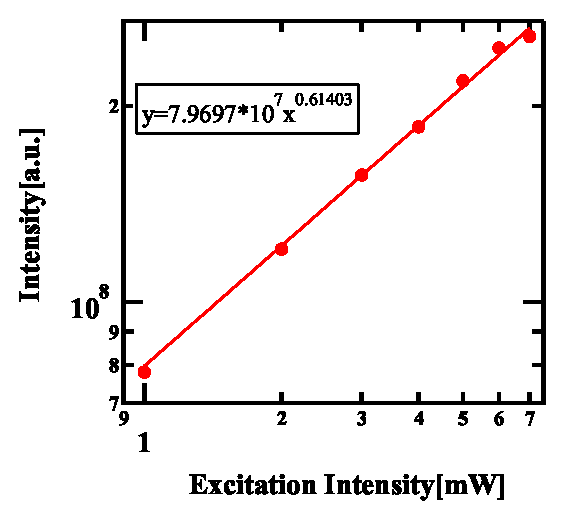
\includegraphics[clip,width=9cm]{start2_CdS_imp_Int.eps}
 \caption{室温のCdSの励起光強度と発光強度の関係.}
 \label{fig_cds_imp_int1}
\end{figure}

縦軸は発光強度、横軸は励起光強度である。発光強度と励起光強度の関係を、$y=\mathrm{A}x^{B}$の形で表す。$B$の値が1を大きく下回っていることと、発光の光子エネルギーが、CdSのエネルギーギャップに比べ小さいことから、このピークはCdS結晶中の不純物由来であることがうかがえる。励起光強度が増加すると、不純物準位が飽和を起こす。つまり、発光強度の増加量に対し、不純物準位からの発光の増加量は小さい。そのため、$B$の値が小さくなる。

%ここからガリヒ素
\newpage
\subsubsection{実験2.2. GaAsの発光スペクトルの励起光強度依存性}

室温のGaAsに波長632.8 nmのレーザーを照射して得られた発光スペクトルを測定した。結果を図\ref{fig_gaas_rt_spec1}に示す。実験2.2.では、得られたデータに対しフィルター感度補正を行った。既知の感度曲線がなかったため、分光器感度補正は行わなかった。

\begin{figure}[ht]
 \centering
 \begin{tabular}{c}

  \begin{minipage}{0.52\hsize}

   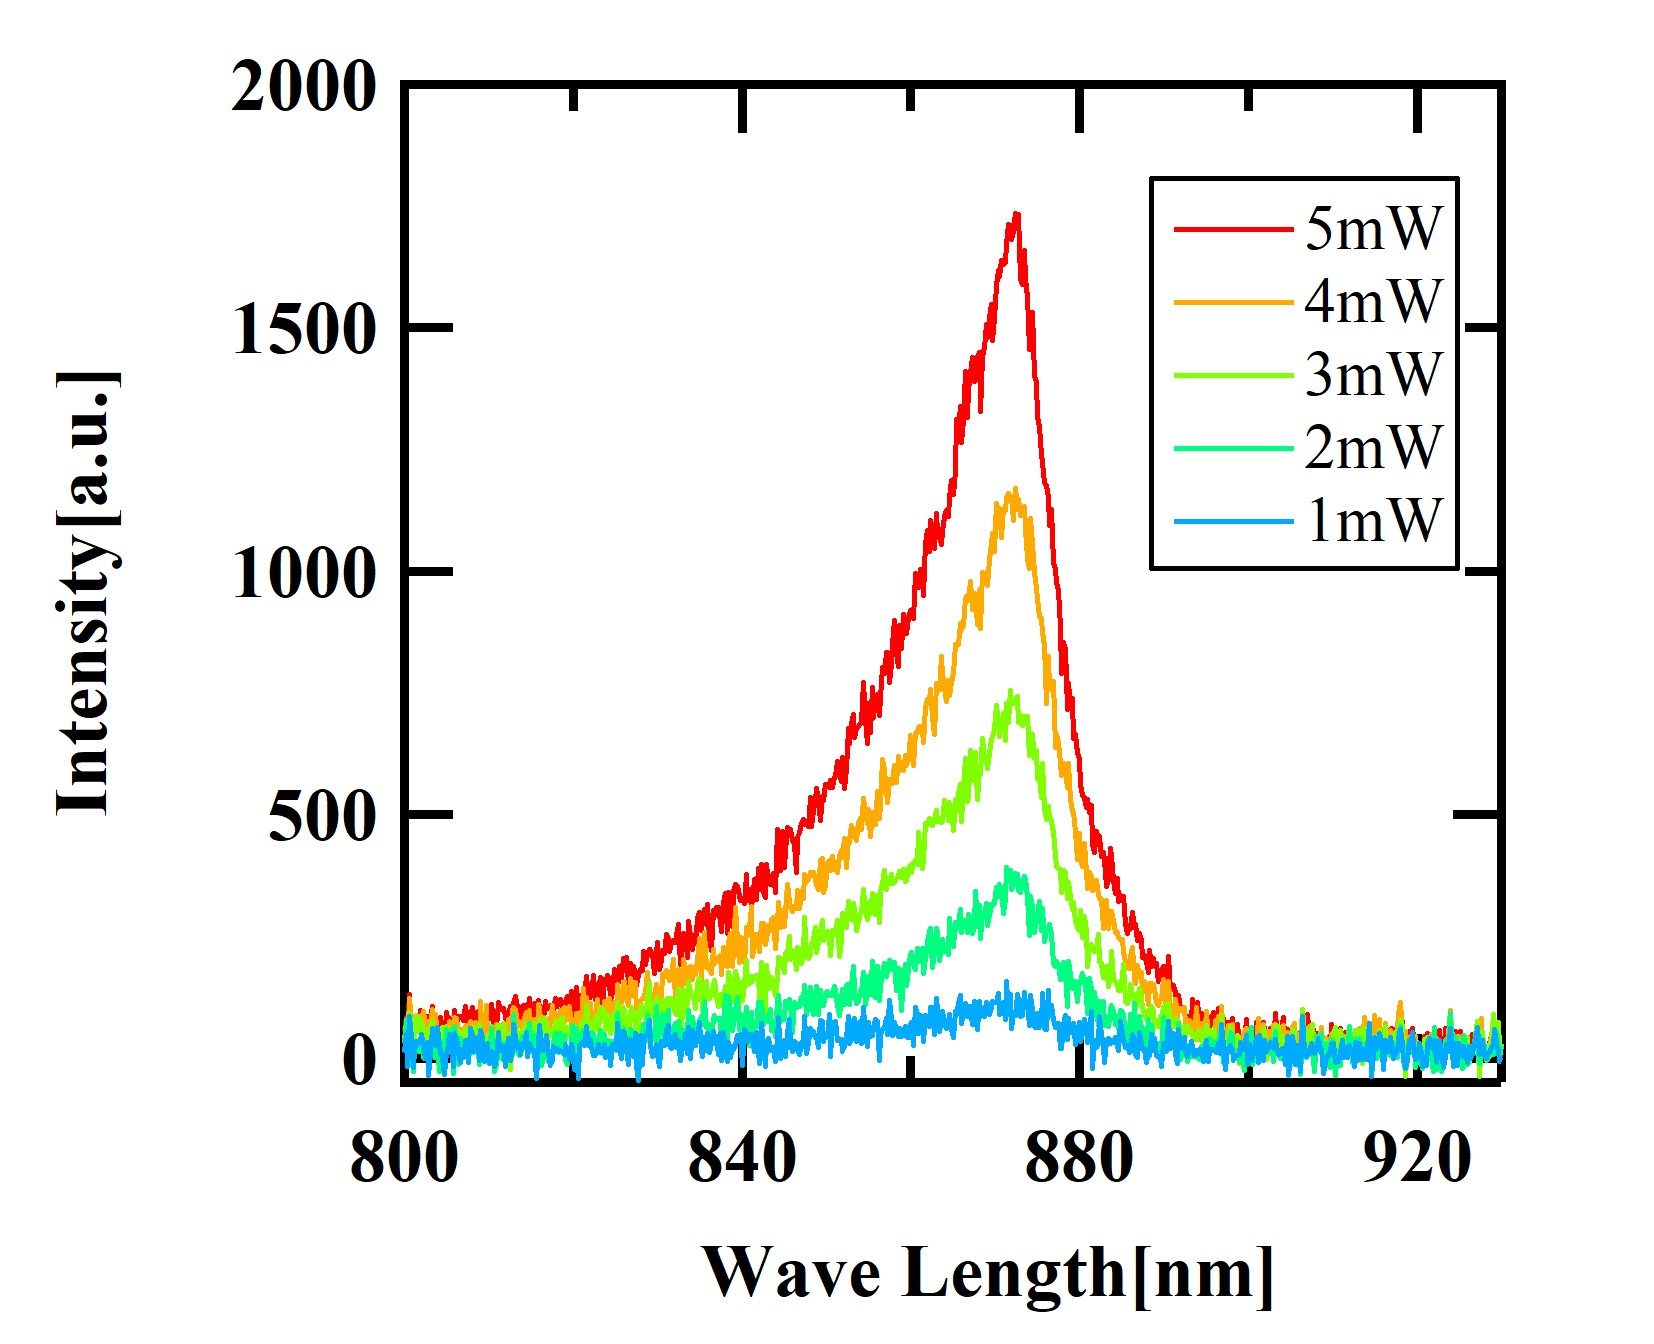
\includegraphics[clip,width=8cm]{start2_GaAs_rt_Spectrum_wav.jpg}
  \end{minipage}

  \begin{minipage}{0.5\hsize}
   \centering
   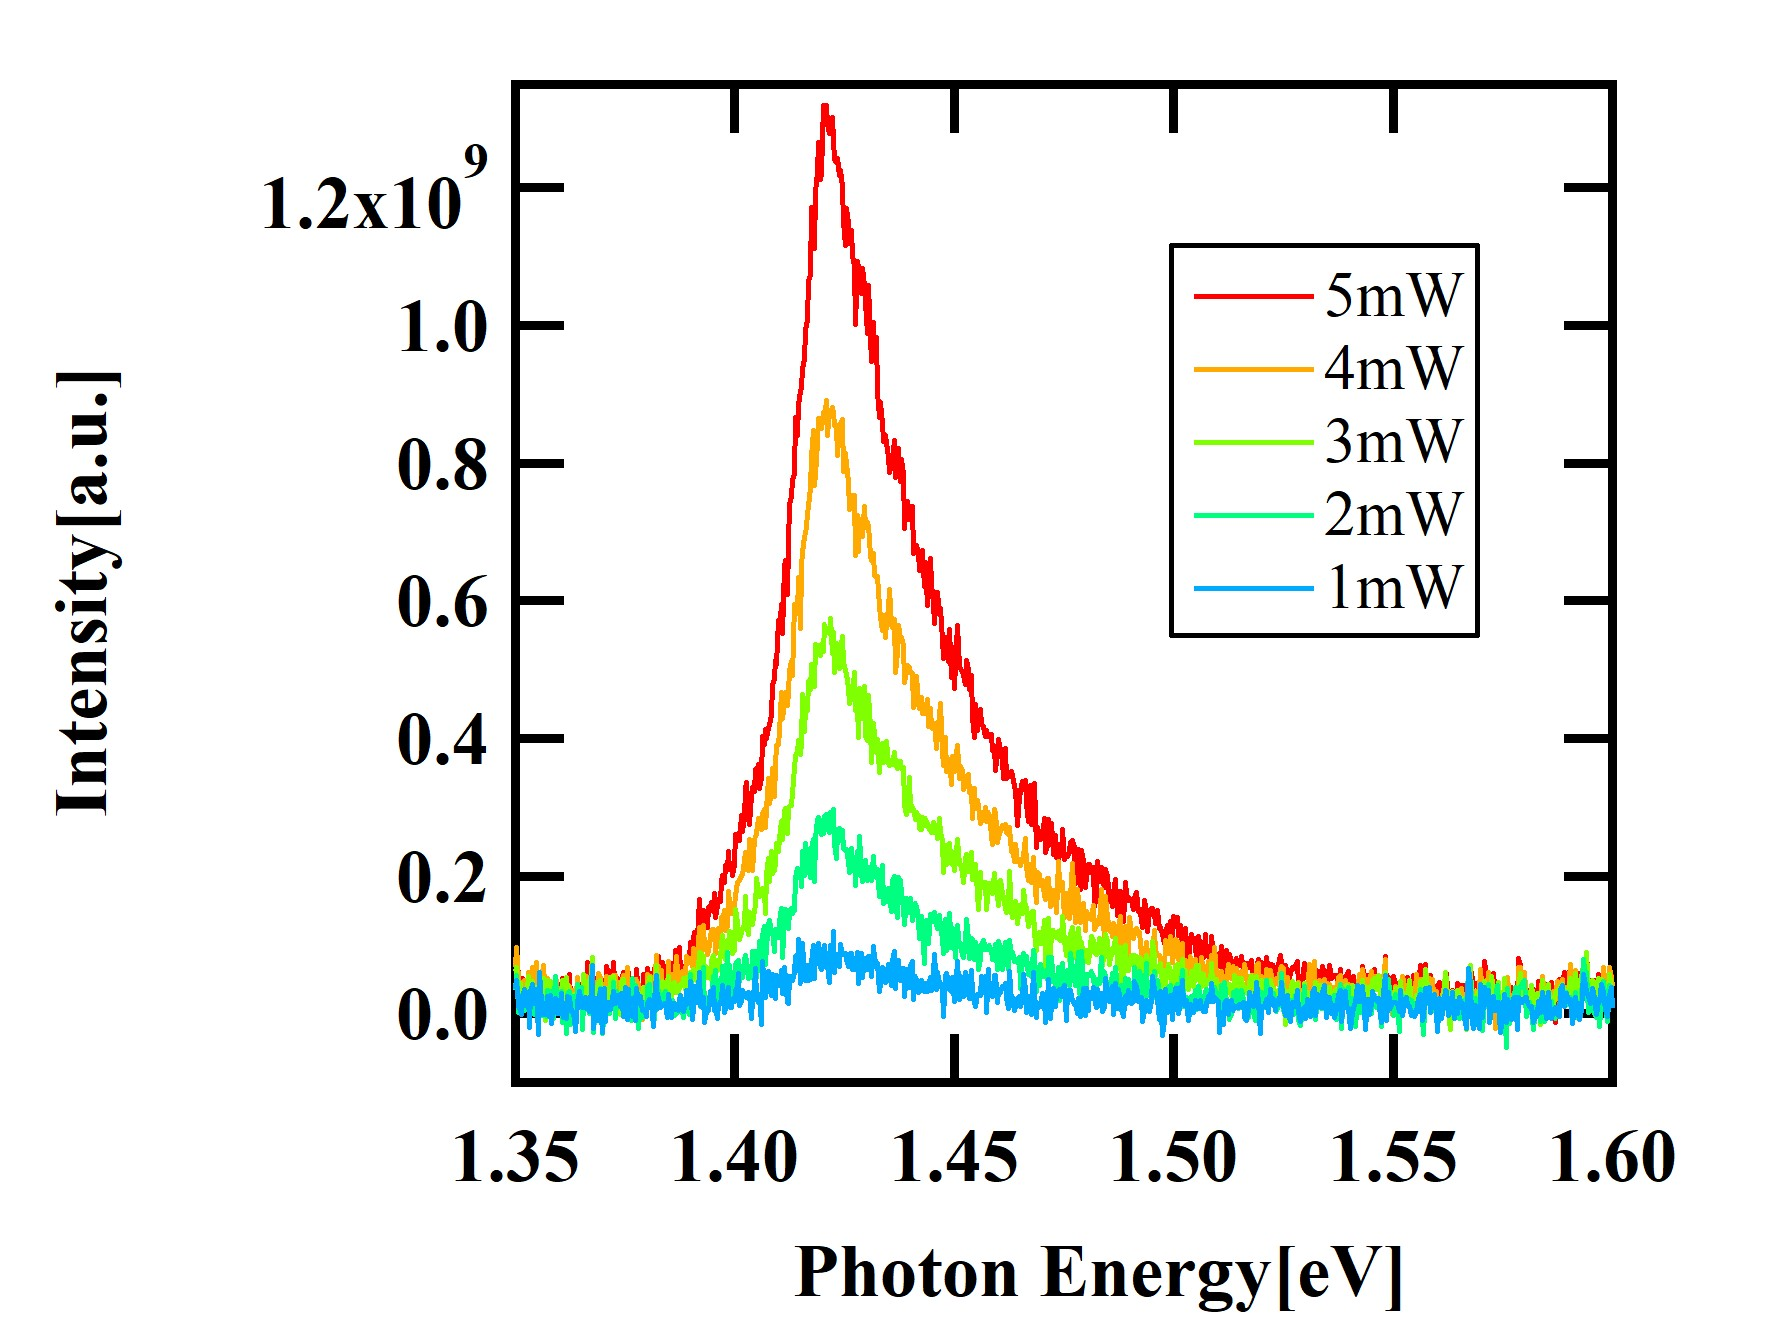
\includegraphics[clip,width=8.3cm]{start2_GaAs_rt_Spectrum_eV.jpg}
  \end{minipage}
 \end{tabular}
 \caption{室温のGaAsにおける発光スペクトル.}
 \label{fig_gaas_rt_spec1}

\end{figure}

縦軸はどちらも発光強度である。左図の横軸は波長、右図の横軸は光子エネルギーである。いずれの励起光強度においても、波長875 nm(エネルギー換算で1.43 eV)付近にピークがある。室温のGaAsのエネルギーギャップは1.43 eVであり\cite{gapE}、スペクトルのピークのエネルギーと一致している。
%各励起光強度におけるピークエネルギーを図\ref{fig_gaas_rt_peak1}に示す。

%\begin{figure}[ht]
%	\centering
%	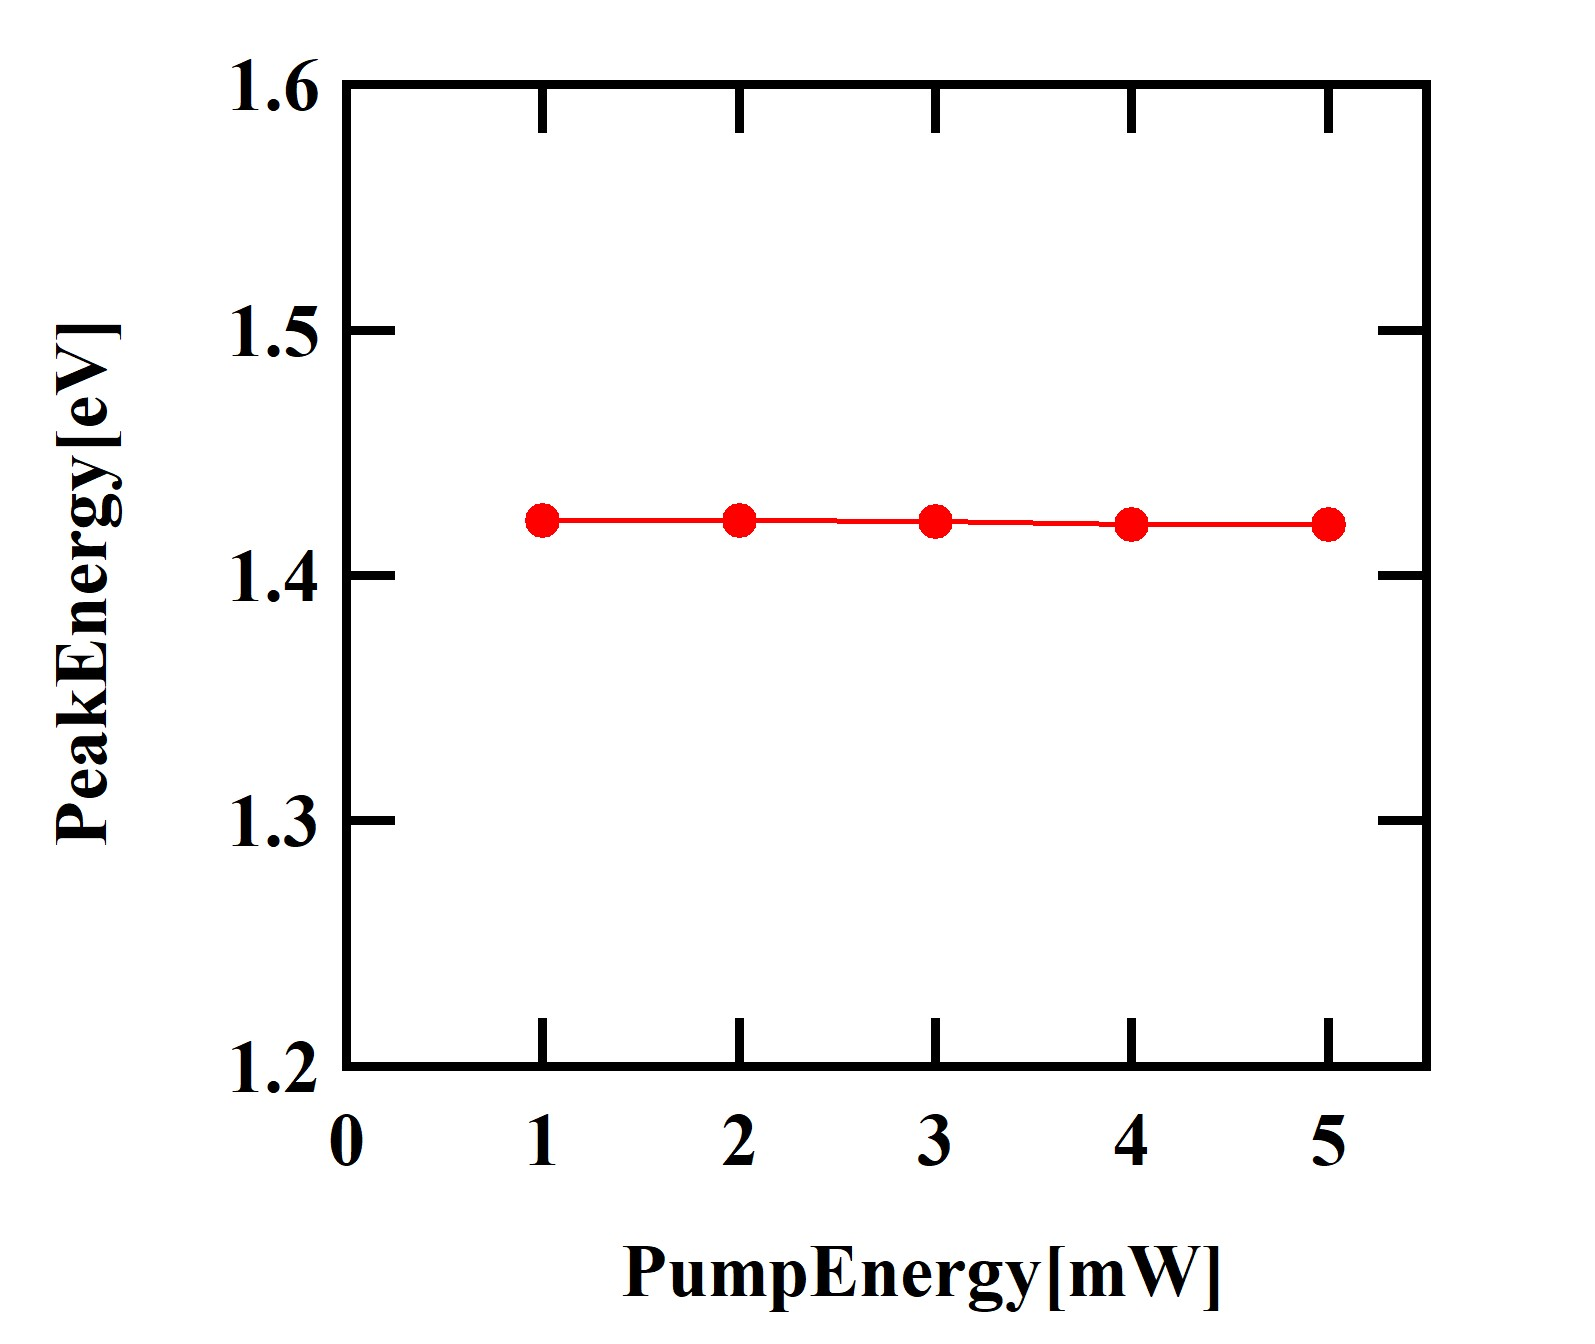
\includegraphics[clip,width=9cm]{start2_GaAs_rt_Peak.jpg}
%	\caption{室温のGaAsの、エネルギー域1.35 eVから1.60 eVの発光スペクトルにおける励起光強度とピークエネルギーの関係.}
%	\label{fig_gaas_rt_peak1}
%\end{figure}

励起光強度が大きくなるにつれて、発光強度が大きくなっていることが読み取れる。励起光強度の大きさと発光強度の大きさの関係を図\ref{fig_gaas_rt_int1}に示す。
\newpage

\begin{figure}[ht]
 \centering
 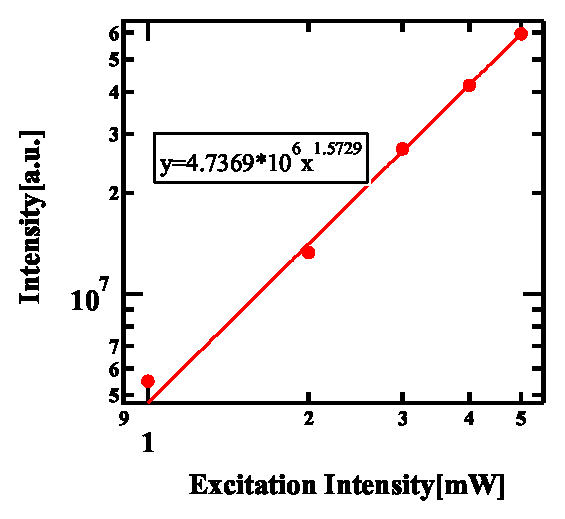
\includegraphics[clip,width=8.5cm]{start2_GaAs_rt_Int.eps}
 \caption{室温のGaAsの発光スペクトルにおける励起光強度と発光強度の関係.}
 \label{fig_gaas_rt_int1}
\end{figure}

縦軸は発光強度で、横軸は励起光強度である。発光強度と励起光強度の関係を、$y=\mathrm{A}x^{B}$の形で表す。$B$の値は1.57である。GaAs中の励起子の束縛エネルギーは4.3 meVである\cite{exciton}。つまり、室温ではGaAs中に励起子は形成されない。励起子が形成されない場合、伝導帯の電子と価電子帯の正孔は相関なく動く。励起光強度が増えると、励起される電子が増えるため、再結合が起こる場合の数が指数的に増加する。そのため、$B$の値は1を上回っている。


室温のGaAsの発光スペクトルを見てみると、ピークの両側で裾を引いているのがわかる。この形状は伝導帯の電子密度が由来である。この形状について、図\ref{fig_lumine1}のように発光スペクトルを2つに分けて考える。

\newpage

\begin{figure}[h]
 \centering
 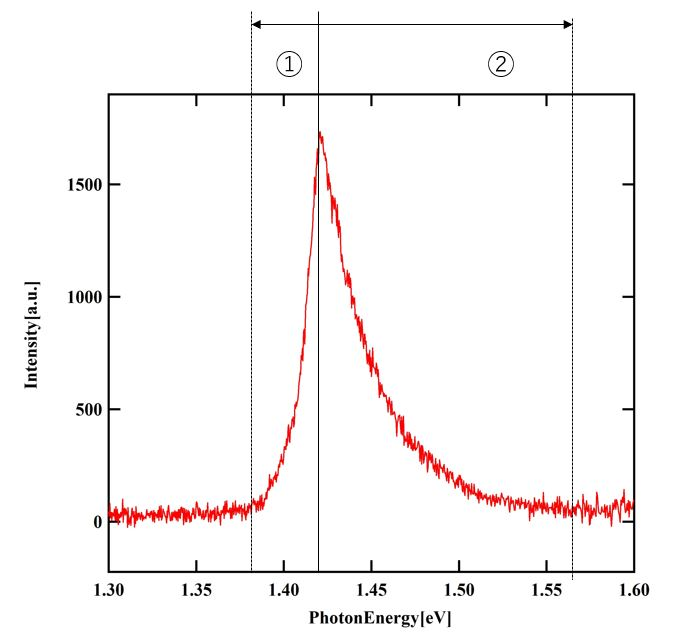
\includegraphics[clip,width=10cm]{start_lumine.jpg}
 \caption{室温のGaAsの発光スペクトル.}
 \label{fig_lumine1}
\end{figure}

電子密度$n$は、状態密度関数$Z_{n}(E)$と分布関数$f_{n}(E)$を用いて
\begin{equation}
 n=Z_{n}(E)\times f_{n}(E)
 \label{eq_spectrum}
\end{equation}
で表される。図\ref{fig_lumine1}のスペクトルのうち、\centercircle{1}の範囲は状態密度関数を反映して鋭く立ち上がり、\centercircle{2}の範囲は分布関数を反映して緩やかに下っている。
%ここもうちょっと考察増やせ

\newpage
\subsubsection{実験2.3. GaAs/AlGaAs量子井戸の発光スペクトルの励起光強度依存性}

\begin{enumerate}%ここからここから箇条書き
 \item 試料温度が室温の時

       室温のGaAs/AlGaAs多重量子井戸に波長632.8 nmのレーザーを照射て得られた発光スペクトルを測定した。結果を図\ref{fig_mqw_rt_spec1}に示す。実験2.3.では、得られたデータに対しフィルター感度補正を行った。既知の感度曲線がなかったため、分光器感度補正は行わなかった。

       \begin{figure}[ht]
        \centering
        \begin{tabular}{c}

         \begin{minipage}{0.52\hsize}

          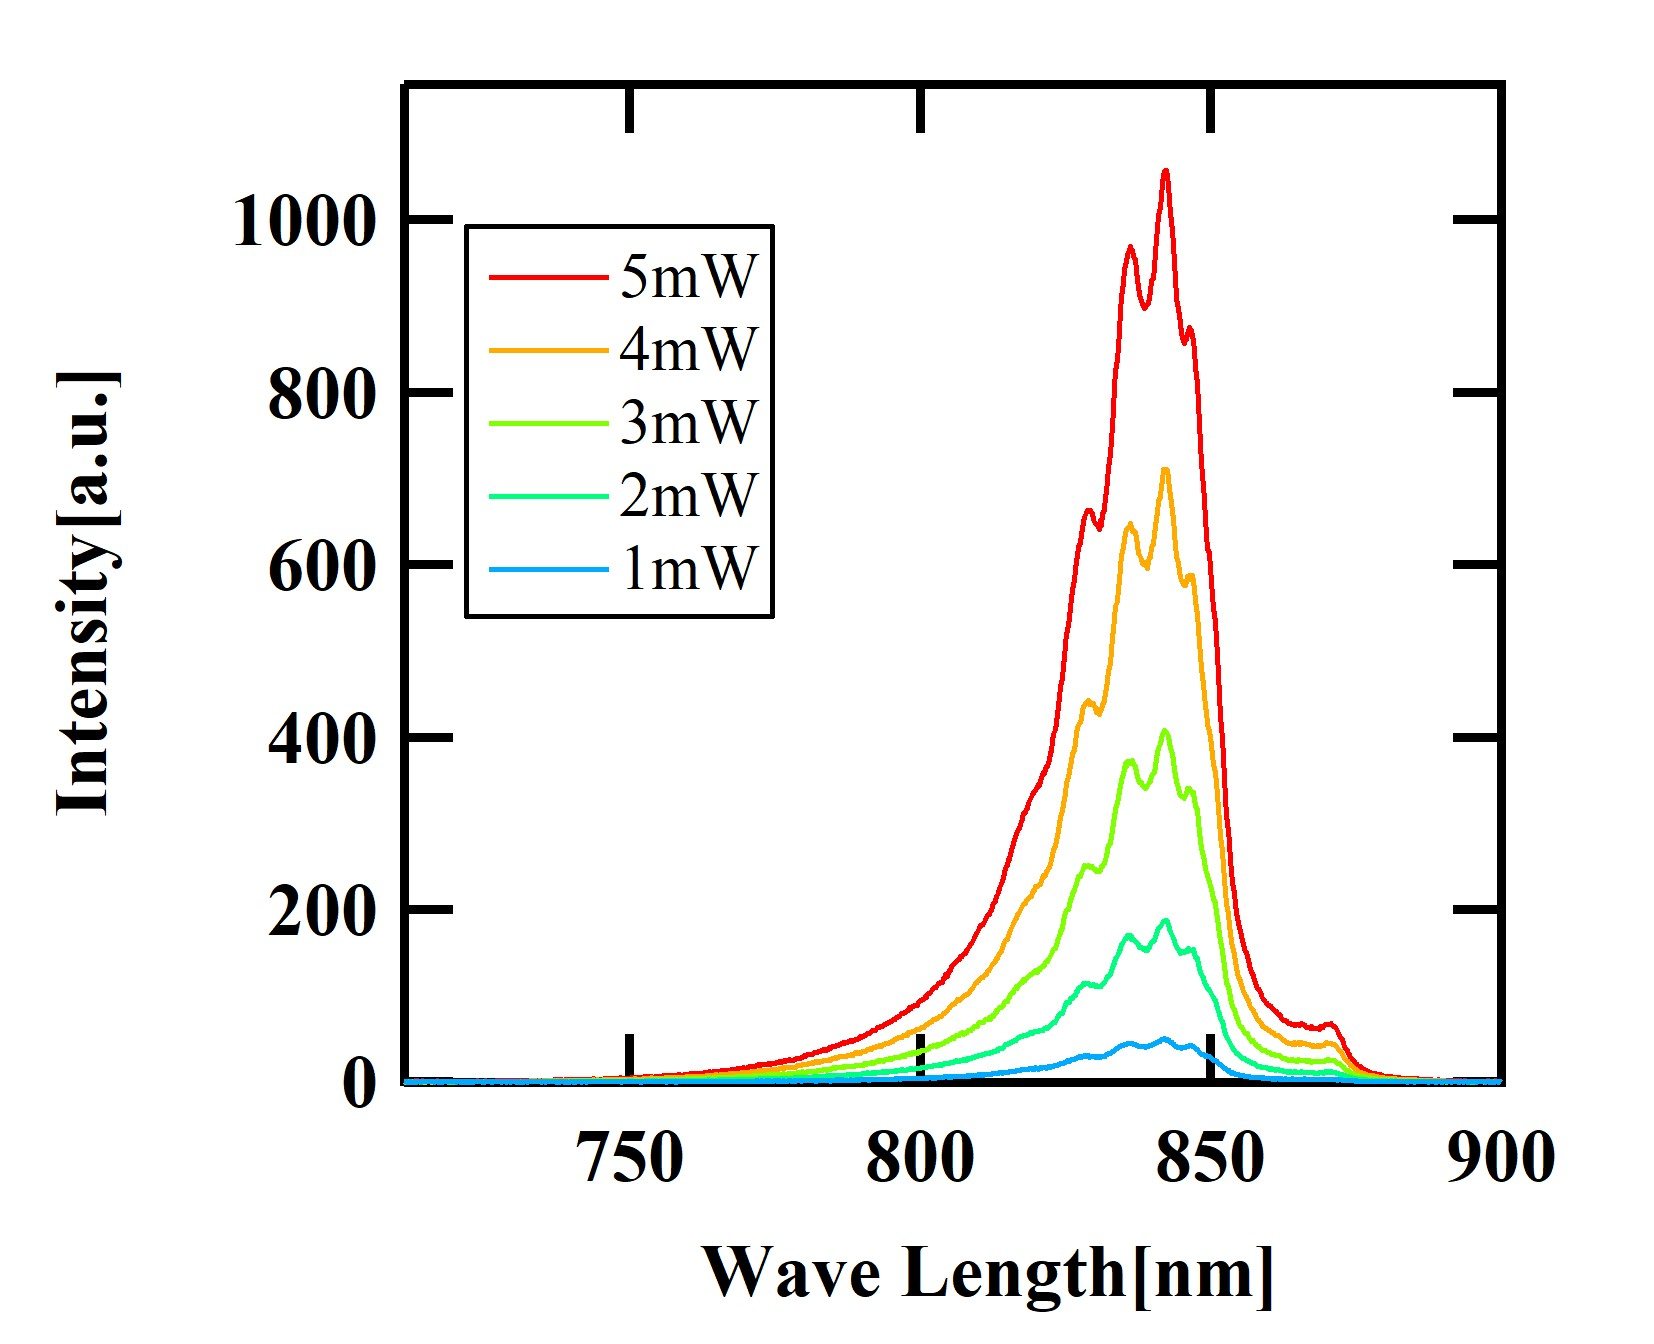
\includegraphics[clip,width=8cm]{start2_MQW_rt_Spectrum_wav.jpg}
         \end{minipage}

         \begin{minipage}{0.5\hsize}
          \centering
          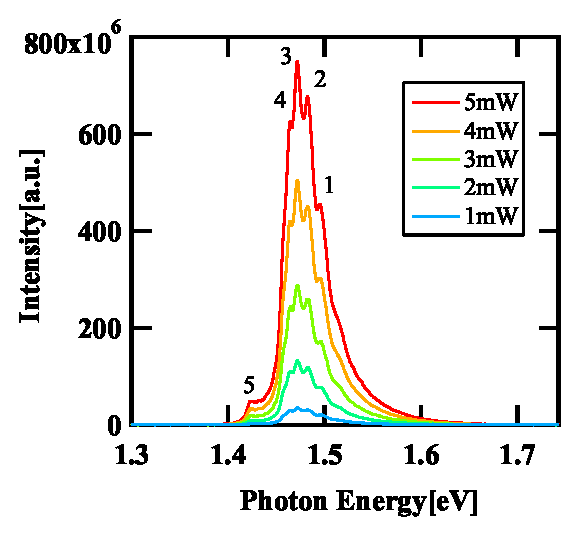
\includegraphics[clip,width=8.3cm]{start2_MQW_rt_Spectrum_eV.eps}
         \end{minipage}
        \end{tabular}
        \caption{室温のMQWにおける発光スペクトル.}
        \label{fig_mqw_rt_spec1}

       \end{figure}


       縦軸はどちらも発光強度である。左図の横軸は波長、右図の横軸は光子エネルギーである。グラフから、ピークが複数読み取れる。これは試料の多重量子井戸構造によるものである。光子エネルギーの高い順に1、2、...と番号を割り振って、各励起光強度におけるそれぞれのピークエネルギーを図\ref{fig_mqw_rt_peak1}に示す。

       \begin{figure}[ht]
        \centering
        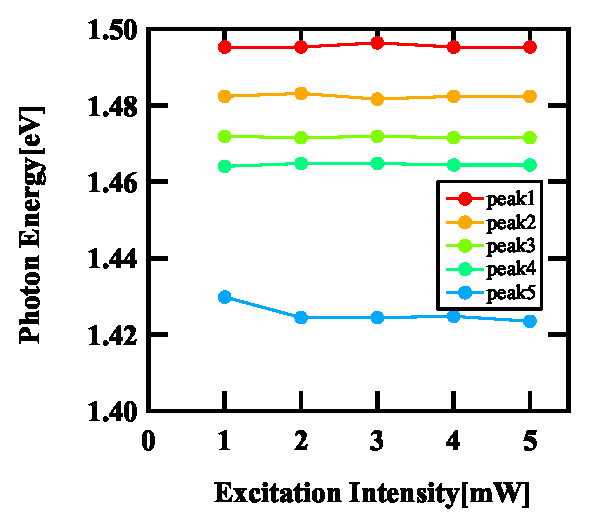
\includegraphics[clip,width=9cm]{start2_MQW_rt_Peak.eps}
        \caption{室温のMQWの発光スペクトルにおける励起光強度とピークエネルギーの関係.}
        \label{fig_mqw_rt_peak1}
       \end{figure}


       % 励起光強度が大きくなるにつれて、発光強度が大きくなっていることも読み取れる。励起光強度の大きさと発光強度の大きさの関係を図\ref{fig_mqw_rt_int1}に示す。

       %\begin{figure}[ht]
       %	\centering
       %	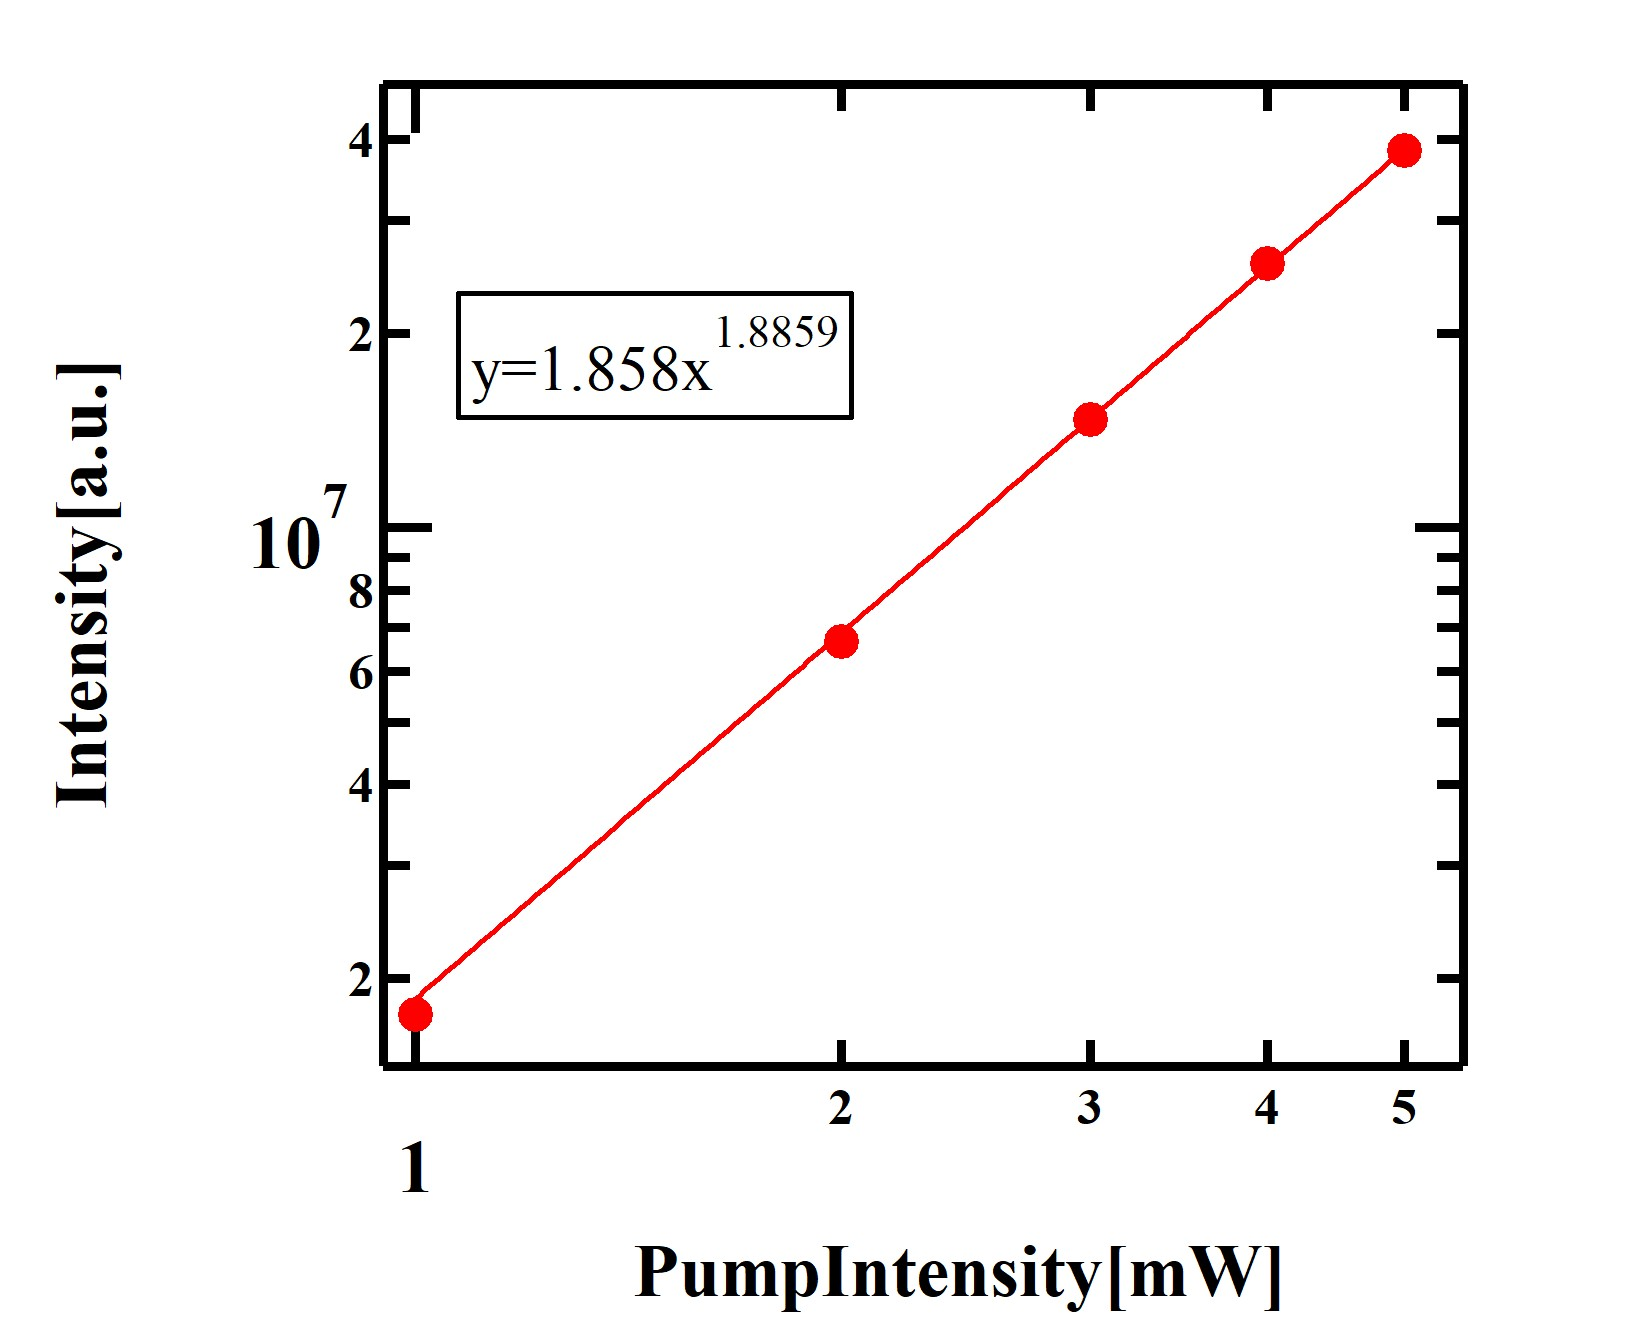
\includegraphics[clip,width=8.5cm]{start2_MQW_rt_Int.jpg}
       %	\caption{室温のMQWの、エネルギー域1.30 eVから1.70 eVの発光スペクトルにおける励起光強度と発光強度の関係.}
       %	\label{fig_mqw_rt_int1}
       %\end{figure}
       %

       \newpage

       縦軸は光子エネルギーで、横軸は励起光強度である。式(\ref{eq_qw})より、量子井戸の幅によって発光の光子エネルギーに差がでる。今回用いた量子井戸は全部で6種類の井戸幅を持つあるため、6つのピークが観測できるはずだが、室温における発光スペクトルでは観測ができていない。これは、室温程度の高温では各個の発光スペクトルが幅を持つため、発光強度が小さいものが埋もれてしまっているからである。したがって、発光スペクトルが鋭くなる低温では、すべてのピークが観測できるはずである。試料温度を77 Kとしたときの結果を次ページから示す。

       \newpage
 \item 試料温度が77 Kの時

       77KのGaAs/AlGaAs量子井戸に波長632.8 nmのレーザーを照射して得られた発光を測定した。結果を図\ref{fig_mqw_77_spec1}に示す。実験2.3.では、得られたデータに対しフィルター感度補正を行った。既知の感度曲線がなかったため、分光器感度補正は行わなかった。


       \begin{figure}[ht]
        \centering
        \begin{tabular}{c}

         \begin{minipage}{0.52\hsize}

          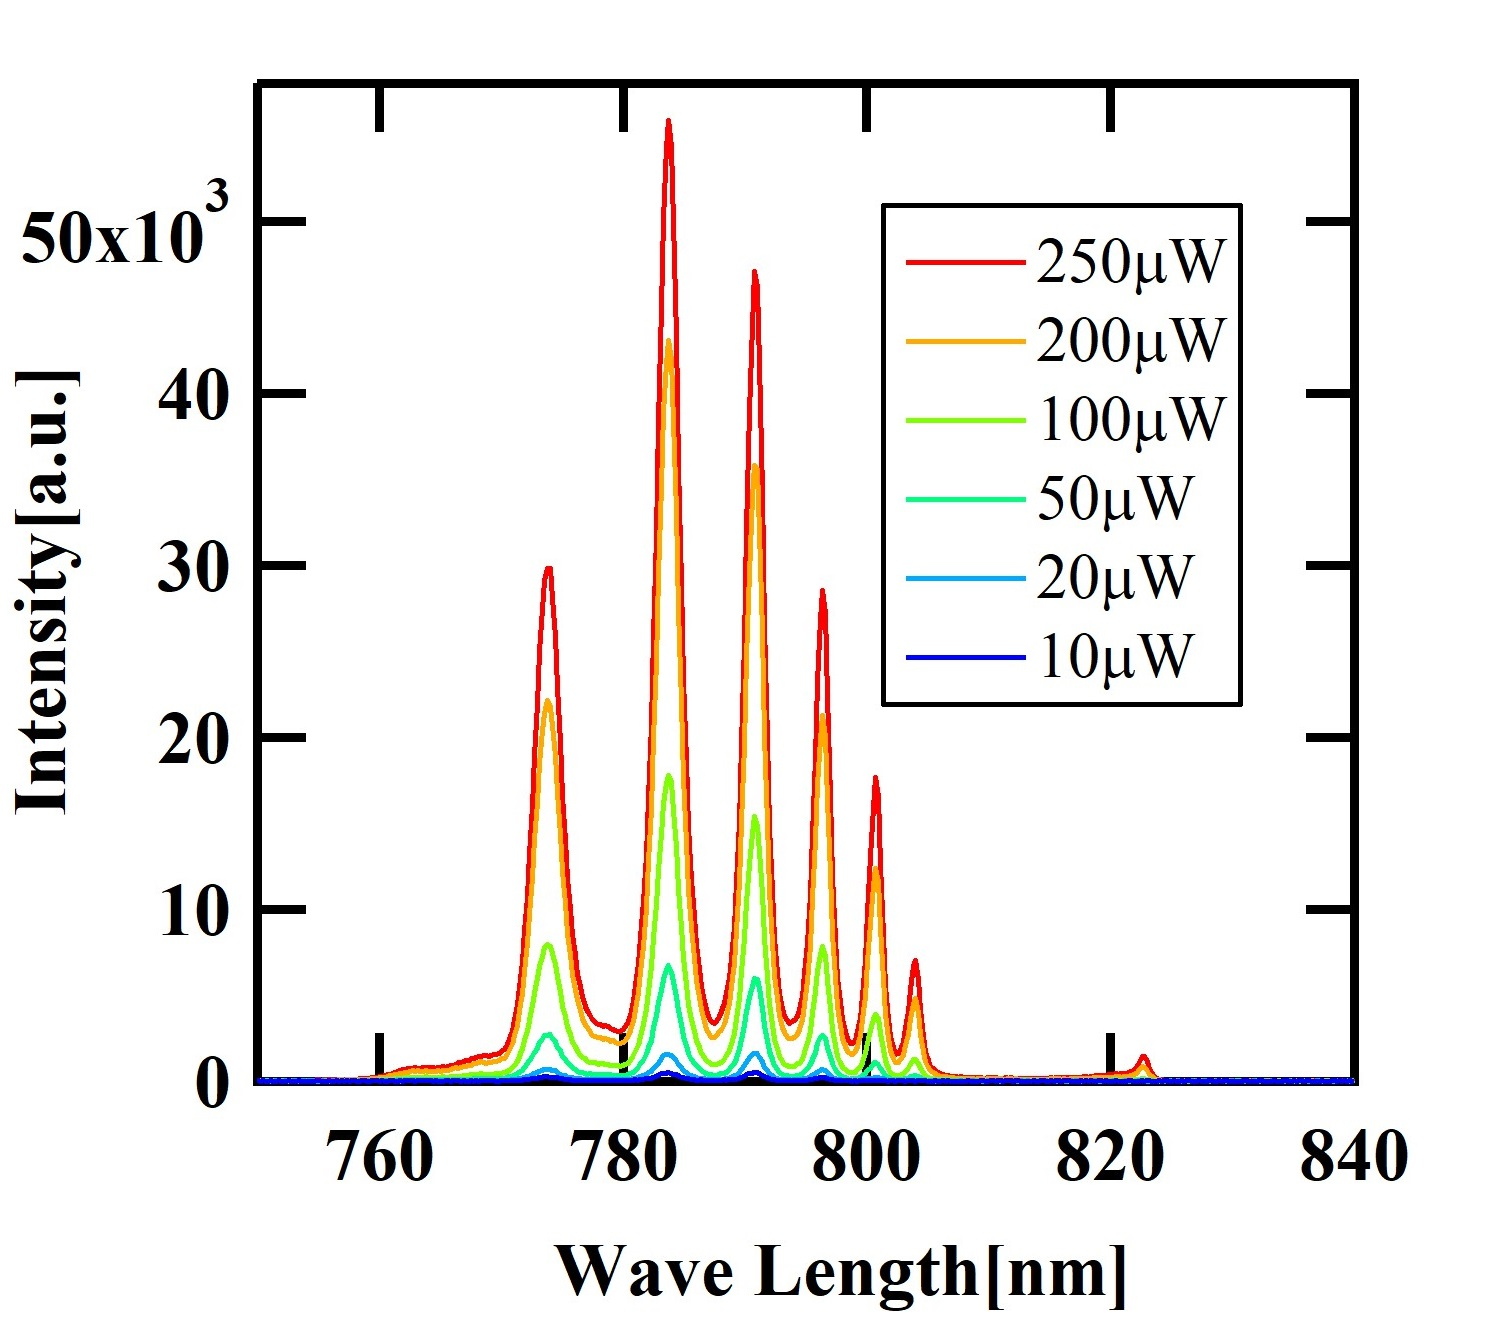
\includegraphics[clip,width=8cm]{start2_MQW_77K_Spectrum_wav.jpg}
         \end{minipage}

         \begin{minipage}{0.5\hsize}
          \centering
          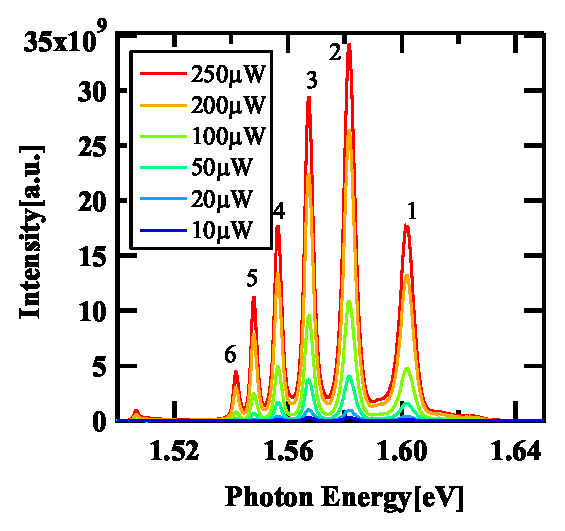
\includegraphics[clip,width=8.3cm]{start2_MQW_77K_Spectrum_eV.eps}
         \end{minipage}
        \end{tabular}
        \caption{77KのMQWにおける発光スペクトル.}
        \label{fig_mqw_77_spec1}

       \end{figure}


       縦軸はどちらも発光強度である。左図の横軸は波長、右図の横軸は光子エネルギーである。グラフから、ピークが複数読み取れる。エネルギーの高い順に1、2、...と番号を割り振った。各励起光強度におけるそれぞれのピークエネルギーを図\ref{fig_mqw_77_peak1}に示す。

       \begin{figure}[ht]
        \centering
        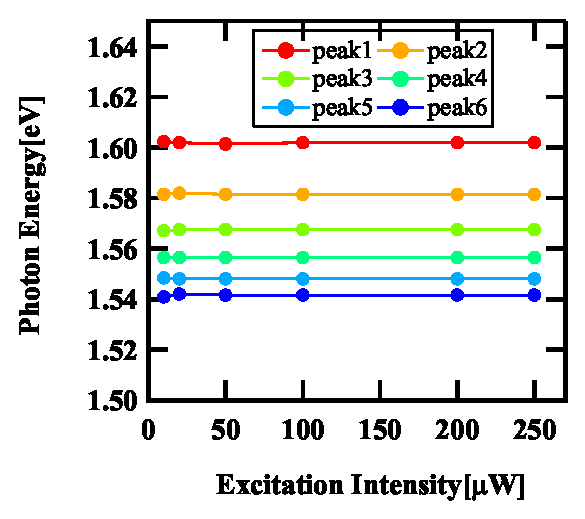
\includegraphics[clip,width=9cm]{start2_MQW_77K_Peak.eps}
        \caption{77KのMQWの発光スペクトルにおける励起光強度とピークエネルギーの関係.}
        \label{fig_mqw_77_peak1}
       \end{figure}

       \newpage

       % また、励起光強度が大きくなるにつれて、発光強度が大きくなっていることも読み取れる。それぞれのピークにおける励起光強度の大きさと発光強度の大きさの関係を図\ref{fig_mqw_77_eg1}に示す。

       %\begin{figure}[ht]
       %	\centering
       %	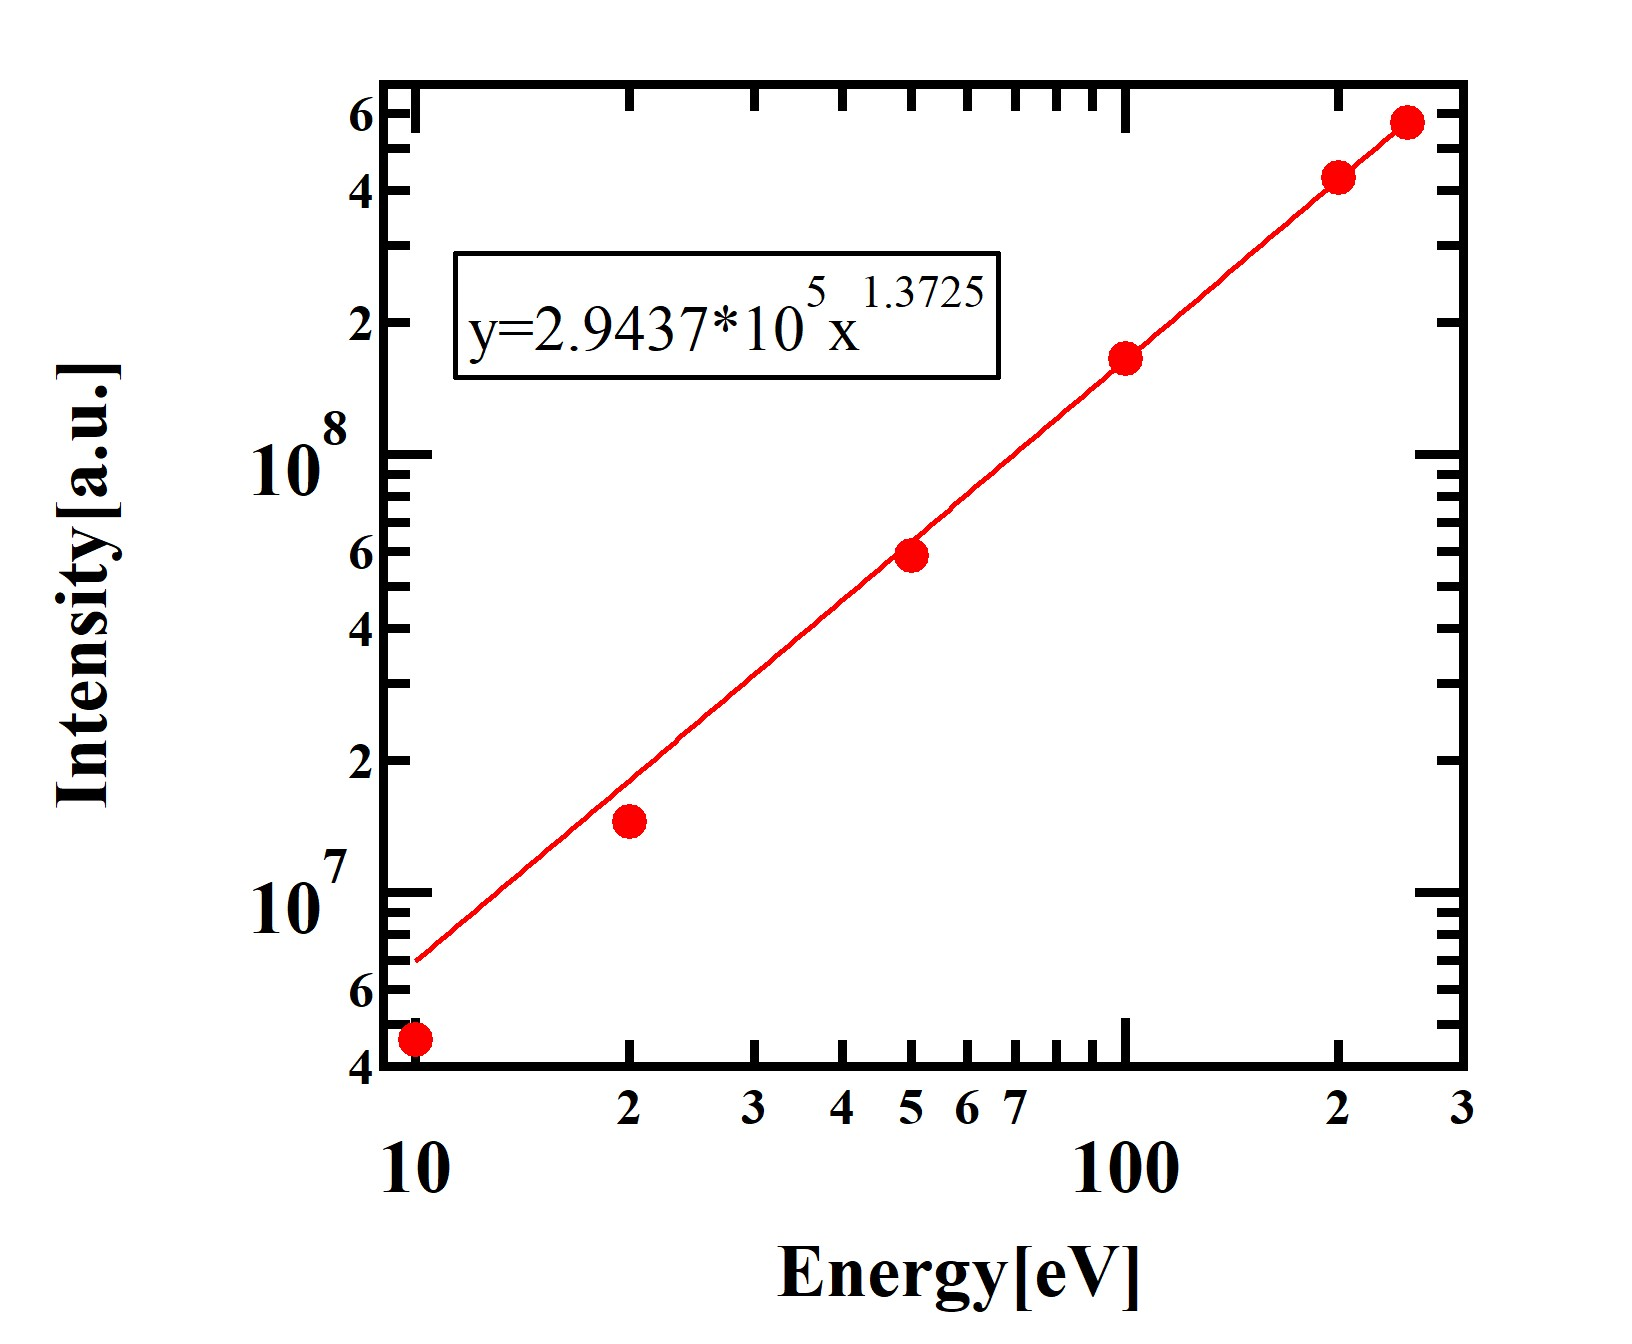
\includegraphics[clip,width=9cm]{start2_MQW_77K_Int.jpg}
       %	\caption{77KのMQWの、エネルギー域1.50 eVから1.65 eVの発光スペクトルにおける励起光強度と発光強度の関係.}
       %	\label{fig_mqw_77_int1}
       %\end{figure}
       %

       縦軸は光子エネルギーで、横軸は励起光強度である。光子エネルギーが高くなるにつれて、ピークどうしの間隔が大きくなっていることがわかる。量子井戸では、井戸幅が狭いほど、エネルギーギャップは小さい。ピークエネルギーと量子井戸の厚さの関係を図\ref{fig_mqw_77_eg1}に示す。

       \newpage

       \begin{figure}[ht]
        \centering
        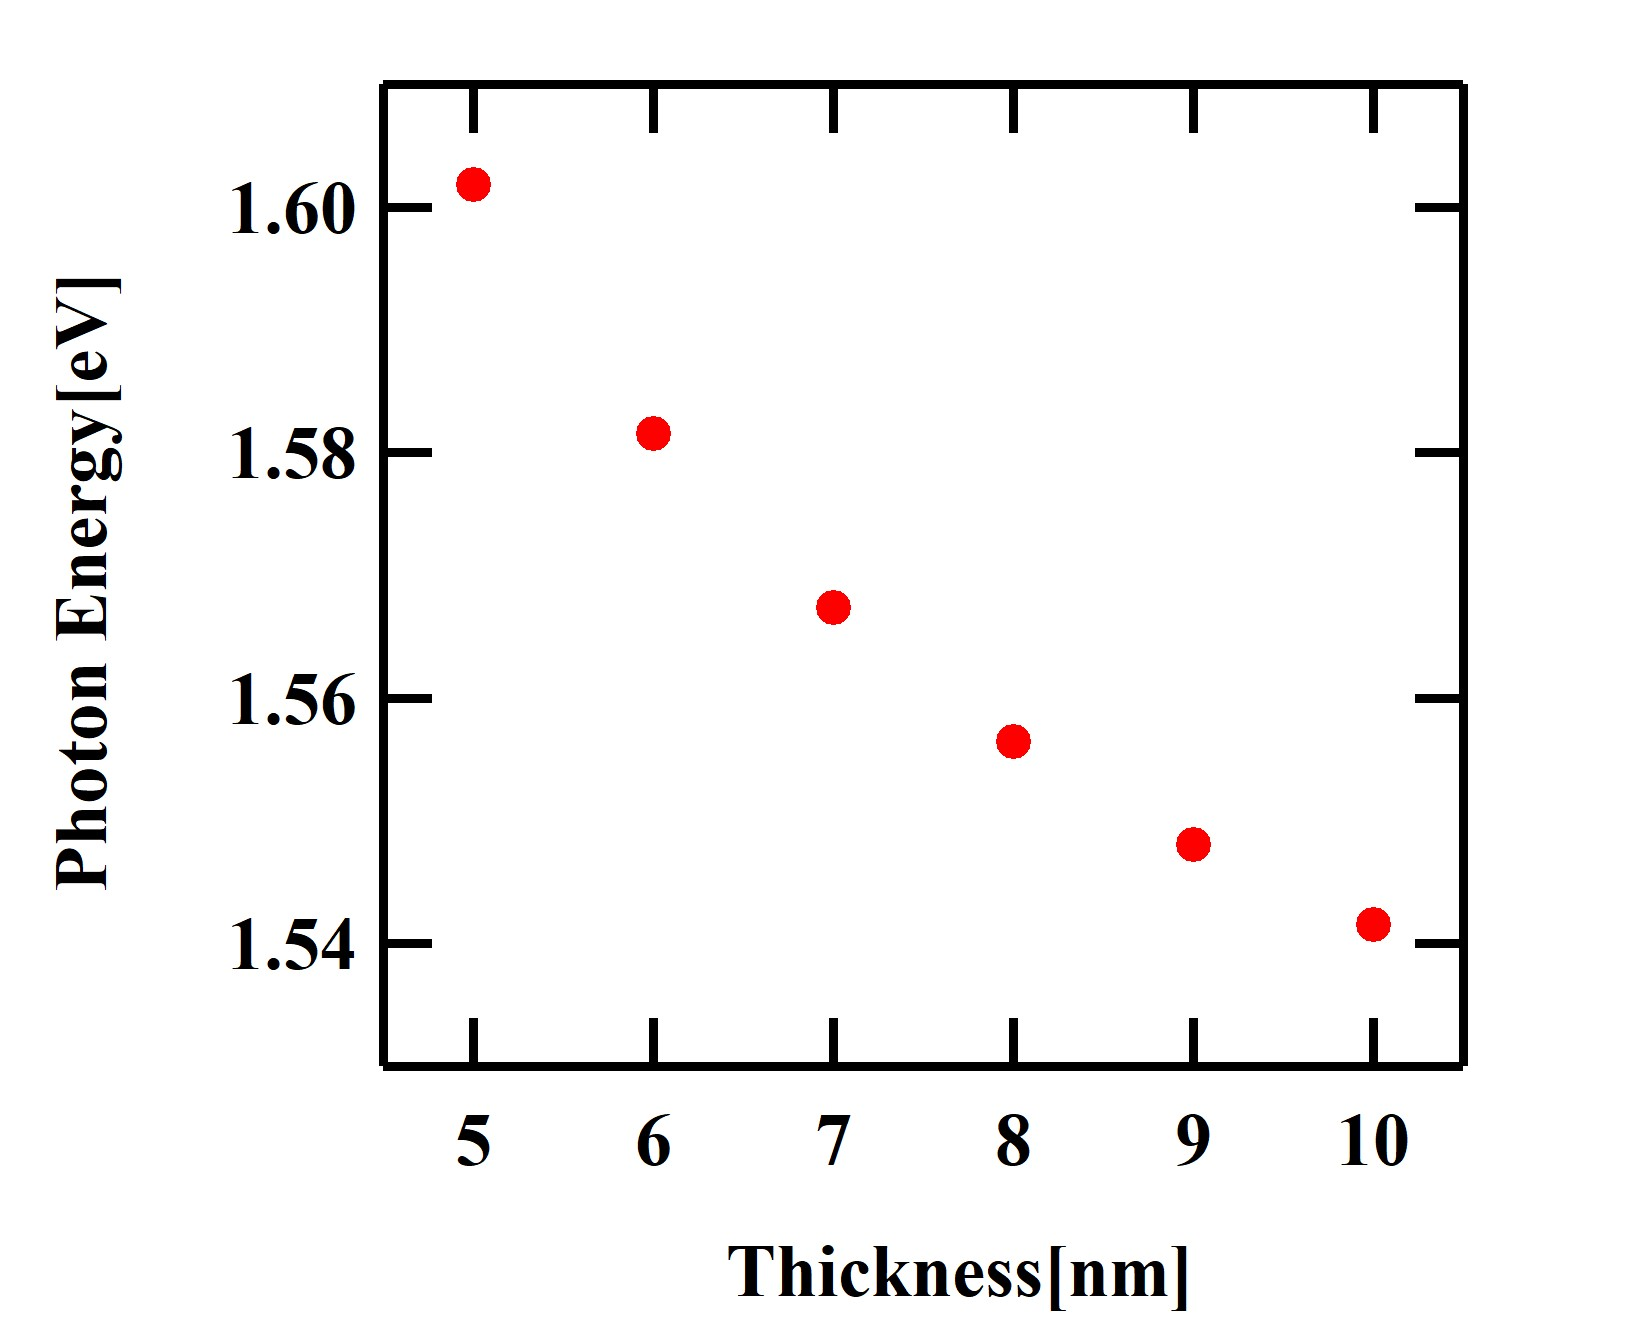
\includegraphics[clip,width=9cm]{start2_MQW_77K_Eg.jpg}
        \caption{量子井戸の厚さと発光エネルギーの関係.}
        \label{fig_mqw_77_eg1}
       \end{figure}

       %、式(\ref{eq_varshni})より
       縦軸は光子エネルギーで、横軸は量子井戸の厚さである。77 KにおけるGaAsのバンドギャップは1.513 eVである。そのため、図\ref{fig_mqw_77_eg1}の縦軸の値から1.513を引けば、量子井戸における、エネルギーギャップとサブバンドとのエネルギー差$\Updelta E$と量子井戸の厚さの関係がわかる。その関係を図\ref{fig_mqw_77_welllength1}に示す。

       \newpage

       \begin{figure}[ht]
        \centering
        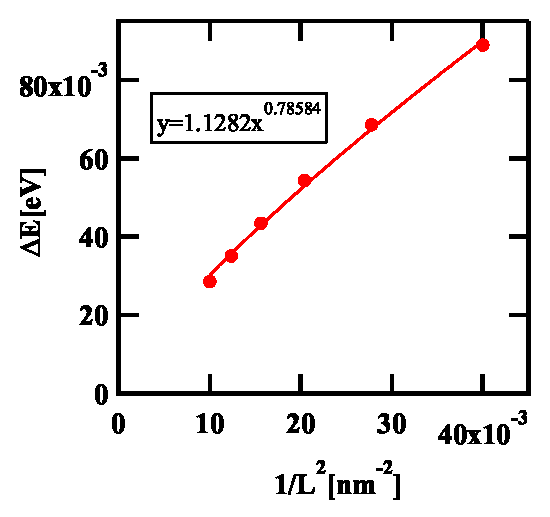
\includegraphics[clip,width=9cm]{start2_MQW_77K_wellLength.eps}
        \caption{量子井戸の厚さとエネルギー差の関係.}
        \label{fig_mqw_77_welllength1}
       \end{figure}

       縦軸は、量子井戸の底とサブバンドの間のエネルギー差である。横軸は、量子井戸の厚さの自乗の逆数である。式(\ref{eq_qw})により、量子井戸の底とサブバンドの間のエネルギー差と、量子井戸の厚さの自乗の逆数は比例関係である。しかし、グラフを見ると、井戸幅が狭くなるほど比例関係から外れ、エネルギー差が小さい値となっている。その理由として、励起子の存在が挙げられる。

       77 KのGaAsのエネルギーギャップは1.513 eV、井戸幅10 nmの時のエネルギーギャップとサブバンドとのエネルギー差$\Updelta E$は37 meVである。したがって、励起子が形成されないとき、ピーク6は1.55 eV付近に観測されると考えられる。しかし、図\ref{fig_mqw_77_spec1}のピーク6は、光子エネルギー1.54 eV付近にあり、計算よりもエネルギーが低い。このことから、GaAs量子井戸中には励起子が存在していることが考えられる。GaAsの励起子の束縛エネルギーは4.3 meVなので、77 KのGaAsバルク中に励起子は存在できない。しかし、GaAsの量子井戸の励起子束縛エネルギーの値は、GaAsバルクの値と異なる。

       GaAsにおいて形成される励起子の有効ボーア半径は13 nmである\cite{exciton}。これは、励起子を形成する電子と正孔の空間的広がりを示す数値である。今回用いたGaAs量子井戸の井戸幅は、最も広くて10 nmである。井戸幅が有効ボーア半径の2倍よりも狭いとき、この井戸幅に収まるように励起子が収縮される。励起子が収縮されると、電子と正孔の間に働くクーロン引力が強くなるため、励起子束縛エネルギーが増大する。井戸幅が狭いほど束縛エネルギーが大きくなるため、$\Updelta E$がその分小さくなる。

       量子井戸における励起子束縛エネルギーは、励起子の有効ボーア半径と井戸幅の2つに依存性を持つ。束縛エネルギーの大きさは、有効ボーア半径と井戸幅の相対比で定まる\cite{bohr}。井戸幅が有効ボーア半径の2倍よりも狭いとき、量子閉じ込め効果が顕著に発現する。
       %\newpage

       %\begin{figure}[ht]
       %\centering
       %  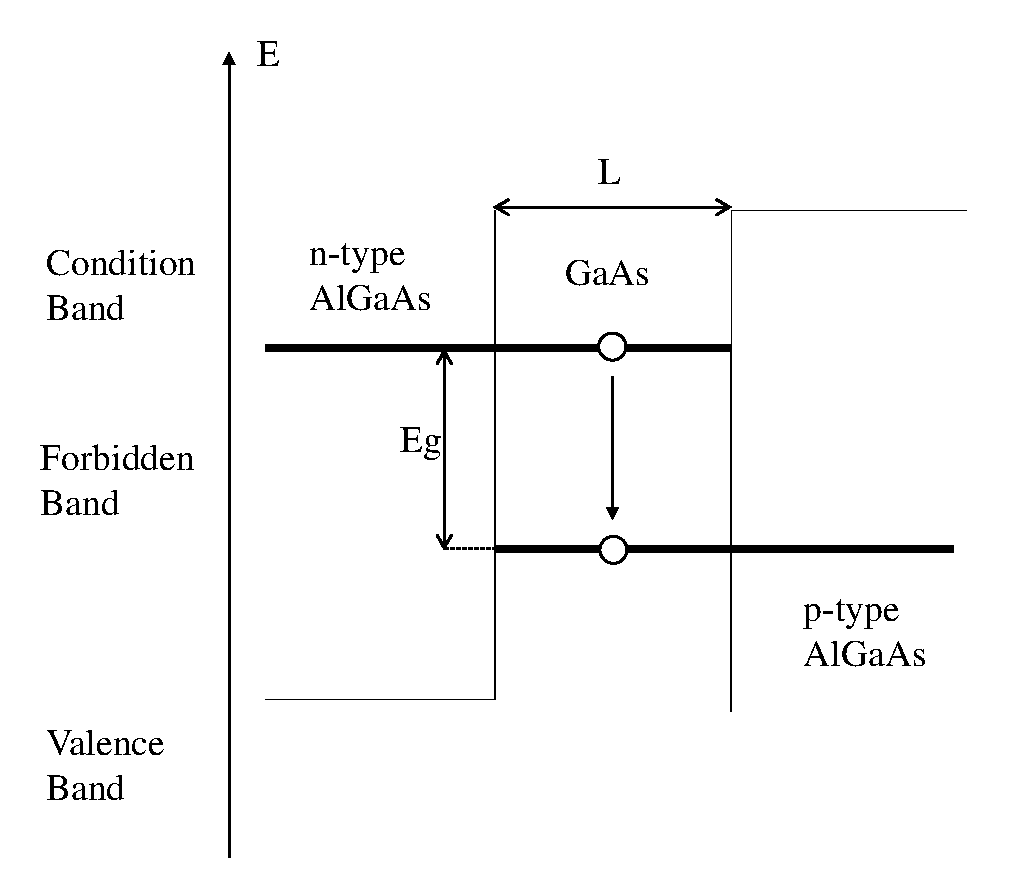
\includegraphics[clip,width=9cm]{start_double.eps}
       %	\caption{ダブルヘテロ構造のバンド図.}
       %  \label{fig_hetero1}
       % \end{figure}

       % ナノサイズのGaAsを、GaAsよりもエネルギーギャップの大きいAlGaAsで挟む。GaAsの部分をコア層、AlGaAsの部分をクラッド層と呼ぶ。AlGaAsの片方をn型、もう片方をp型半導体とする。n型AlGaAsとGaAsの伝導帯の最低エネルギー準位が揃っているとき、電子はコア層にたまる。同様に、p型AlGaAsとGaAsの価電子帯の最高エネルギー準位がそろっているとき、正孔はコア層にたまる。そのため、電子と正孔はコア層で再結合がしやすくなる。クラッド層の屈折率がコア層の屈折率より大きいとき、コア層で発生した光子はクラッド層に逃げることができず、コア層に閉じ込められる。コア層に閉じ込められた光は誘導放出を誘発する。そのため、量子井戸をレーザーとして使用することができる。

       %ここから量子井戸の活用についてたくさん

       量子井戸のエネルギーギャップは、バルクにおけるエネルギーギャップとサブバンドとのエネルギー差$\Updelta E$と、励起子束縛エネルギーの2つによって定まることがわかった。この2つのエネルギーは、どちらも井戸幅依存性を持つ。つまり、量子井戸では、試料の井戸幅を変えることで、任意のエネルギーギャップを実現できる。

       量子井戸のこの特性を生かした、量子井戸レーザーというものがある。%量子井戸をレーザーとして用いる際の、2種類の物質の接合パターンの一つに、ダブルヘテロ構造と呼ばれるものがある。ダブルヘテロ構造のバンド図を図\ref{fig_hetero1}に示す。
       量子井戸レーザーの利点として、
       \begin{itemize}
        \item 任意のエネルギーギャップを作れる
        \item しきい値電流が低い
        \item 発光強度の操作がしやすい
       \end{itemize}
       等が挙げられる。1つ目は先ほど述べたとおりである。2つ目は、一つの量子井戸の幅が小さく、そもそもの電子の数が少ないため、反転分布状態が作りやすいためである。しきい値電流とは、レーザー発振が可能な最小の電流である。3つ目は、発光強度は層の数が増えると大きくなるためである。今回の実験で用いた量子井戸は、各井戸幅ごとに5層だったが、より層を重ねることで大きな発光が期待できる。

       図\ref{fig_mqw_77_eg1}の右図には、1.5 eV付近に小さなピークがあることもわかる。その部分を拡大したものを図\ref{fig_mqw_77_1.5ev1}に示す。

       \begin{figure}[ht]
        \centering
        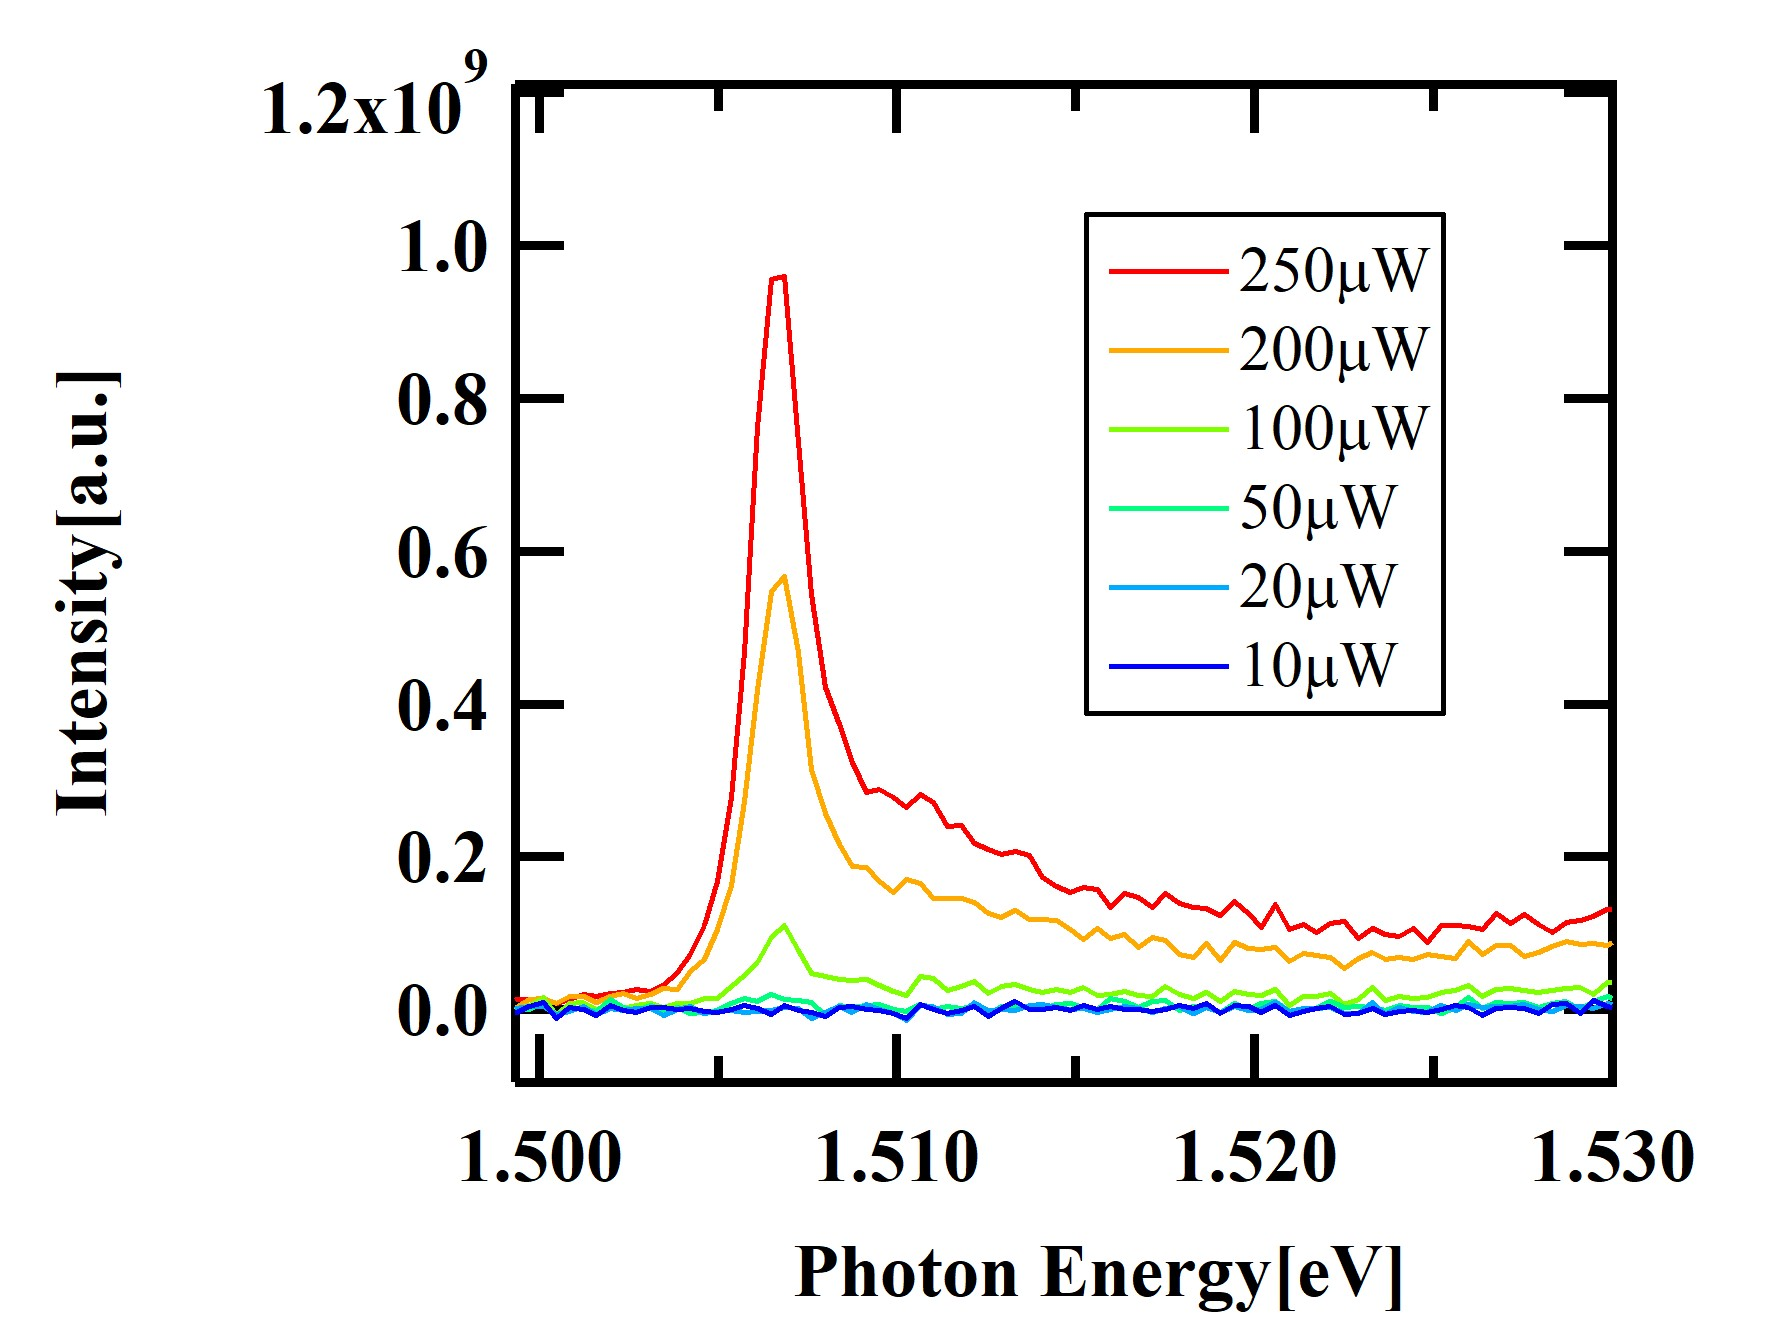
\includegraphics[clip,width=9cm]{start2_MQW_77K_GaAs.jpg}
        \caption{77KのMQWの1.50 eV付近の発光スペクトル.}
        \label{fig_mqw_77_1.5ev1}
       \end{figure}

       縦軸は光強度、横軸は光子エネルギーである。1.508 eVにピークがあることがわかる。これは、試料のGaAs基板による発光だと考えられる。77 KのGaAsバルク中には励起子は存在できないため、図\ref{fig_mqw_77_1.5ev1}のスペクトルは、GaAsのバンド間発光によるものである。

\end{enumerate}%箇条書きここまで.

\newpage
\section{結論}
CdS、GaAs及びGaAs/AlGaAs多重量子井戸の発光の特性を測定した。CdSとGaAsの発光スペクトルと励起光強度の関係及び、GaAs/AlGaAs多重量子井戸のエネルギー準位と井戸幅の関係の解明に成功した。

%参考文献。\cite{タグ}で参照を示せる。
\begin{thebibliography}{9}
 \bibitem{Grating}株式会社島津 https://www.shimadzu.co.jp/products/opt/guide/07.html 2019/4/12
 \bibitem{CCD} キヤノンサイエンスラボ https://global.canon/ja/technology/s\_labo/light/003/04.html 2019/04/12
 \bibitem{Fibor} 分光計器株式会社 http://www.bunkoukeiki.co.jp/technology.fiber.html 2019/04/12
 \bibitem{HeNe}Thorlab\,\,https://www.thorlabs.co.jp/newgrouppage9.cfm?objectgroup\_id=10776 2019/4/15
 \bibitem{varshni}Y.P.Varshni TEMPERATURE DEPENDENCE OF THE ENERGY GAP IN SEMICONDUCTORS
 \bibitem{gapE}キッテル固体物理学入門上第8版 p.119
 %\bibitem{qw}安仁屋勝ほか 量子井戸中における励起子の結合エネルギー http://hdl.handle.net/2433/93527
 \bibitem{exciton}中山正昭 半導体結晶の光学的評価 http://www.a-phys.eng.osaka-cu.ac.jp/hikari-g/nakayama/optical-properties.pdf 2019/4/15
 \bibitem{bohr}吉川喜彬 GaAs/AlAs 多重量子井戸構造における励起子―励起子散乱と
 タイプII超格子における電子・正孔液滴の発光特性に関する研究 http://dlisv03.media.osaka-cu.ac.jp/contents/osakacu/kiyo/111TDA3617.pdf 2019/4/25

\end{thebibliography}

\end{document}
